%%%%%%%%%%%%%%%%%%%%%%%%%%%%%%%%%%%%%%%%%%%%%%%%%%%%%%%%%%
%
% Vzor pro sazbu kvalifikační práce
%
% Západočeská univerzita v Plzni
% Fakulta aplikovaných věd
% Katedra informatiky a výpočetní techniky
%
% Petr Lobaz, lobaz@kiv.zcu.cz, 2016/03/14
%
%%%%%%%%%%%%%%%%%%%%%%%%%%%%%%%%%%%%%%%%%%%%%%%%%%%%%%%%%%

% Možné jazyky práce: czech, english
% Možné typy práce: BP (bakalářská), DP (diplomová)
\documentclass[czech,DP]{thesiskiv}

% Definujte údaje pro vstupní strany
%
% Jméno a příjmení; kvůli textu prohlášení určete, 
% zda jde o mužské, nebo ženské jméno.
\author{Kateřina Kratochvílová}
\declarationfemale

%alternativa: 
%\declarationfemale

% Název práce
\title{Nástroj pro automatickou identifikaci KIR alel}

\thanktext{Ráda bych poděkovala Ing. Lucii Houdové, Ph.D. za cenné rady, věcné připomínky, trpělivost a ochotu, kterou mi v průběhu zpracování této práce věnovala. Dále bych chtěla poděkovat panu Ing. Jiřímu Fatkovi za jeho rady a pomoc při vytváření praktické části. }
% 
% Texty abstraktů (anglicky, česky)
%
\abstracttexten{This masters thesis is focused on the identification of KIR alleles. The aim is to design and implement a tool for their automatic identification. First, the KIR genes and methods used to obtain the genomic data using DNA sequencing - next-generation sequencing (NGS) - were introduced. Secondly, the possible bioinformatic tools were analyzed.
The identification tool was developed on synthetics reads and then tested and verified by commercial DNA data acquired from FN Plzeň / BC LF UK Plzeň. The creation of synthetic reads was done with a help of ART tool and referencial DNA sequence alligning was done by Bowtie2. During the development, several approaches were proposed and evaluated based on their possible application.}

\abstracttextcz{Diplomová práce se zabývá identifikací KIR alel. Cílem práce je návrh a implementace nástroje pro jejich automatickou identifikaci. V práci jsou představeny KIR geny a metody získávaní genomických dat s využitím DNA sekvenace, konkrétně next-generation sequencing (NGS). Dále byly analyzovány využitelné bioinformatické nástroje. Samotný identifikační nástroj byl vyvíjen na syntetických readech a nakonec testován a verifikován na datech komerčních linii DNA získaných z FN Plzeň/BC LF UK Plzeň. Vytváření syntetických readů probíhalo pomocí nástroje ART, pro zarovnávání readů na referenční DNA sekvence byl využit nástroj Bowtie2. V rámci vývoje bylo navrženo několik možných přístupů, které byly poté vyhodnoceny s ohledem na jejich možné využití.
}

% Na titulní stranu a do textu prohlášení se automaticky vkládá 
% aktuální rok, resp. datum. Můžete je změnit:
%\titlepageyear{2016}
%\declarationdate{1. března 2016}

% Ve zvláštních případech je možné ovlivnit i ostatní texty:
%
%\university{Západočeská univerzita v Plzni}
%\faculty{Fakulta aplikovaných věd}
%\department{Katedra informatiky a výpočetní techniky}
%\subject{Bakalářská práce}
%\titlepagetown{Plzeň}
%\declarationtown{Plzni}

%%%%%%%%%%%%%%%%%%%%%%%%%%%%%%%%%%%%%%%%%%%%%%%%%%%%%%%%%%
%
% DODATEČNÉ BALÍČKY PRO SAZBU
% Jejich užívání či neužívání záleží na libovůli autora 
% práce
%
%%%%%%%%%%%%%%%%%%%%%%%%%%%%%%%%%%%%%%%%%%%%%%%%%%%%%%%%%%

% Zařadit literaturu do obsahu
\usepackage[nottoc,notlot,notlof]{tocbibind}

% Umožňuje vkládání obrázků
\usepackage[pdftex]{graphicx}

\usepackage{subcaption}
% Odkazy v PDF jsou aktivní; navíc se automaticky vkládá
% balíček 'url', který umožňuje např. dělení slov
% uvnitř URL
\usepackage[pdftex]{hyperref}
\hypersetup{colorlinks=true,
  unicode=true,
  linkcolor=black,
  citecolor=black,
  urlcolor=black,
  bookmarksopen=true}

% matematicke rovnice %
\usepackage{amsmath}
\usepackage{fancyhdr}
\usepackage{float}
\numberwithin{equation}{section}
% Při používání citačního stylu csplainnatkiv
% (odvozen z csplainnat, http://repo.or.cz/w/csplainnat.git)
% lze snadno modifikovat vzhled citací v textu
\usepackage[numbers,sort&compress]{natbib}

\usepackage{multirow}
\usepackage{multicol}
\usepackage{import}

%tabulky
\usepackage{makecell} 
\usepackage[table]{xcolor} 
\usepackage{pdflscape}
\usepackage{longtable}

%pouzite zkratky
\usepackage{blindtext}
\usepackage{scrextend}
\addtokomafont{labelinglabel}{\sffamily}

%%%%%%%%%%%%%%%%%%%%%%%%%%%%%%%%%%%%%%%%%%%%%%%%%%%%%%%%%%
%
% VLASTNÍ TEXT PRÁCE
%
%%%%%%%%%%%%%%%%%%%%%%%%%%%%%%%%%%%%%%%%%%%%%%%%%%%%%%%%%%
\begin{document}
%
\maketitle
\tableofcontents

\chapter{Úvod}
Transplantace krvetvorných buněk se využívá jako terapeutická procedura pro mnoho vážných hematologických poruch mezi které patří například akutní myeloidní leukemie. Transplantace je proces, při kterém jsou dárci odebrány krvetvorné buňky, které jsou následně vpraveny do těla pacienta trpícího hematologickou poruchou. Jednou z komplikací, která může nastat, je reakce imunitního systému na nově vložené dárcovské buňky resp. štěp. V případě, že si štěp s imunitním systémem nebudou rozumět, může dojít k silné zánětlivé reakci, která může skončit až smrtí pacienta. V neposlední řadě může dojít také k relapsu (návratu) onemocnění. 
\\
\\
K potlačení odmítnutí dárcovského štěpu se primárně vybírají dárci podle shody v HLA znacích následovaných sekundárními znaky, kterými mohou být například věk či pohlaví. Shoda v HLA znacích se určuje podle shody v alelách genů HLA -A, -B, -C, -DRB1, -DQB1. Alela je konkrétní forma genu. Každý jedinec má tyto HLA geny dvakrát (jednu pětici od matky a druhou od otce), a proto se úplná shoda označuje jako 10/10. Nověji je možné se setkat s označením 12/12. Znamená to 10/10 navýšené o gen HLA -DPB1. Tento gen, ale na rozdíl od standarních HLA znaků, nevyžaduje přesnou shodu. Klíčové je zde zda patří do skupiny permisivních (tolerančních) alel, které by měly snížit možnost relapsu (návrat nemoci) a rizika transplantace. Oproti tomu některé skupiny alel naopak mohou rizika zvýšit. V poslední době se objevují studie, které prokazují vliv i takzvaných non-HLA genů. Jedním z nich může být i skupina genů Killer-cell immunoglobulin-like receptor (KIR). Jednou z výhod je, že určité seskupení KIR genů snižuje riziko návratu nemoci. V případě, kdy by se rozhodovalo mezi více dárci shodných v HLA znacích, by se mohl ten vhodnější vybrat právě na základě KIR. Pro zjištění jak HLA znaků tak KIR genů se využívají sekvenační metody. \cite{KIR_transplantace_jindra} \cite{Frycova_bakalarka} \cite{DPB1_houdova}
\\
\\
Cílem práce je navrhnout a implementovat nástroj pro automatickou identifikaci KIR alel. Vstupní data, tzv. ready, jsou krátké kusy DNA (posloupnost písmen A, C, G a T) a jsou výstupem ze sekvenačních technik. Může to být gen, část genu nebo několik různých genů. Tyto ready se zarovnávají vůči referenční alelám. Díky tomu je možné zjistit, o které alely se jedná. Ready budou pro vývoj nástroje simulovány a v konečné fázi testování budou vyměněny za data z FN Plzeň/BC LF UK Plzeň. V poslední fázi bude vyhodnocena shoda readů a referenčních genů.


\chapter{Imunitní systém a jeho spojitost s geny}
Imunitní systém chrání organismus před škodlivinami. Skládá se ze dvou hlavních částí, z vrozené imunity a získané imunity. Reakce imunitního systému je vždy komplexní reakcí organismu, přičemž tato reakce je tvořena jednotlivými buňkami imunitního systému reagující na přítomnost specifických antigenů. Antigeny jsou látky, které imunitní systém rozpozná a zareaguje na ně. V podstatě to může být jakákoli bílkovinná sloučenina. Antigen se obvykle nachází na povrchu buňky jako vyjádření genu. Imunitní systém následně zjistí o jaký antigen se jedná, respektive o jakou buňku se jedná, zda tělu vlastní (např. zdravá buňka) nebo buňku tělu cizí (např. nádorová buňka), tedy jedná-li se o expresi lidského genu nebo například viru. Jedná-li se o buňku tělu cizí, imunitní systém reaguje snahou ji zničit. 
\\
\\
\textbf{Vrozená imunita}, též označována přirozená, neadaptivní, antigenně nespecifická je neměnně zapsána v DNA. To znamená, že při každém setkání s antigenem odpoví stejnou reakcí. Buňky nesoucí vrozenou imunitu jsou stále přítomny v krvi, takže jejich případná aktivace je takřka okamžitá (minuty až hodiny). Do této imunity patří i natural killer buňky s KIR receptory, kterým bude věnována pozornost dále v textu. 
\\
\\
\textbf{Získaná imunita}, též označována specifická či adaptivní, má oproti specifické v genomu zapsány pouze své základy. V průběhu lidského života se vyvíjí a mění. Změna může nastat například očkováním nebo proděláním patřičné choroby. Tato změna ovšem nemusí být trvalá. Z těchto důvodů může být odpověď ziskané imunity při setkání se stejnou chorobou rozdílná. Fungování získané imunity zajišťují T- a B- lymfocyty. Získaná imunita nefunguje samostatně. Při zabíjení patogenů spolupracuje s vrozenou imunitou.

\section{Geny}
V každé buňce lidského organismu, konkrétně v buněčném jádře, se nachází 46 chromozomů. Jeden chromozom představuje stočenou dlouhou molekulu DNA (Deoxyribonuklenovou kyselinu). Všech 46 chromozomů obsahuje okolo 100 000 genů. Genem se rozumí drobný segment DNA, který řídí buněčnou funkci. Konkrétní forma genu je alela. \citep{en_smith}

\begin{figure}[H]		
		\centering
		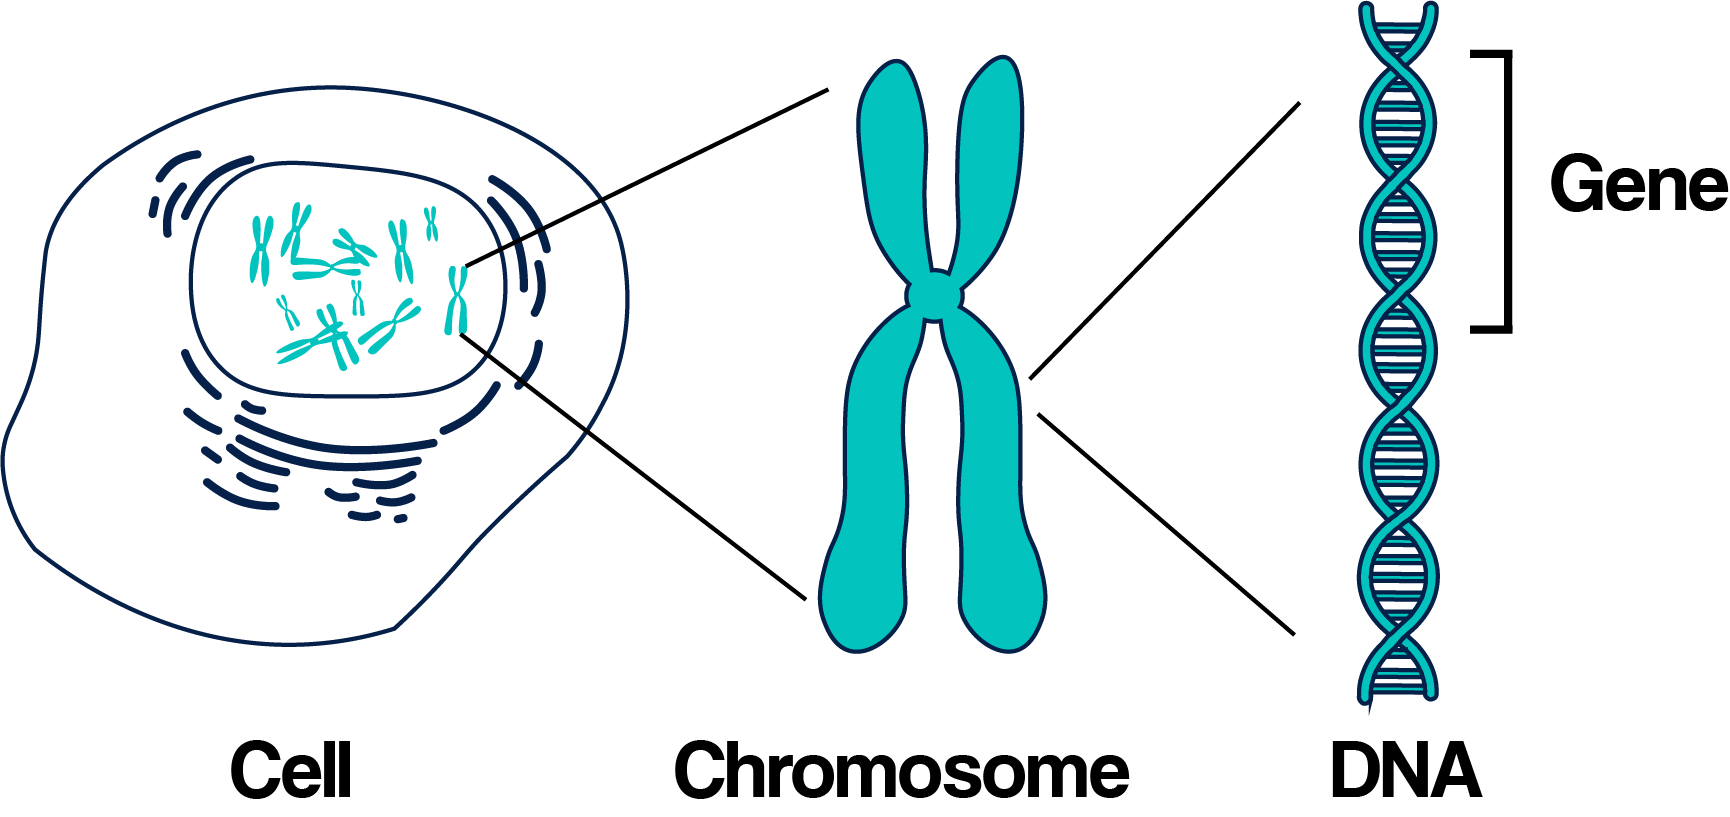
\includegraphics[width=150px]{./img/lidska_bunka.png}
		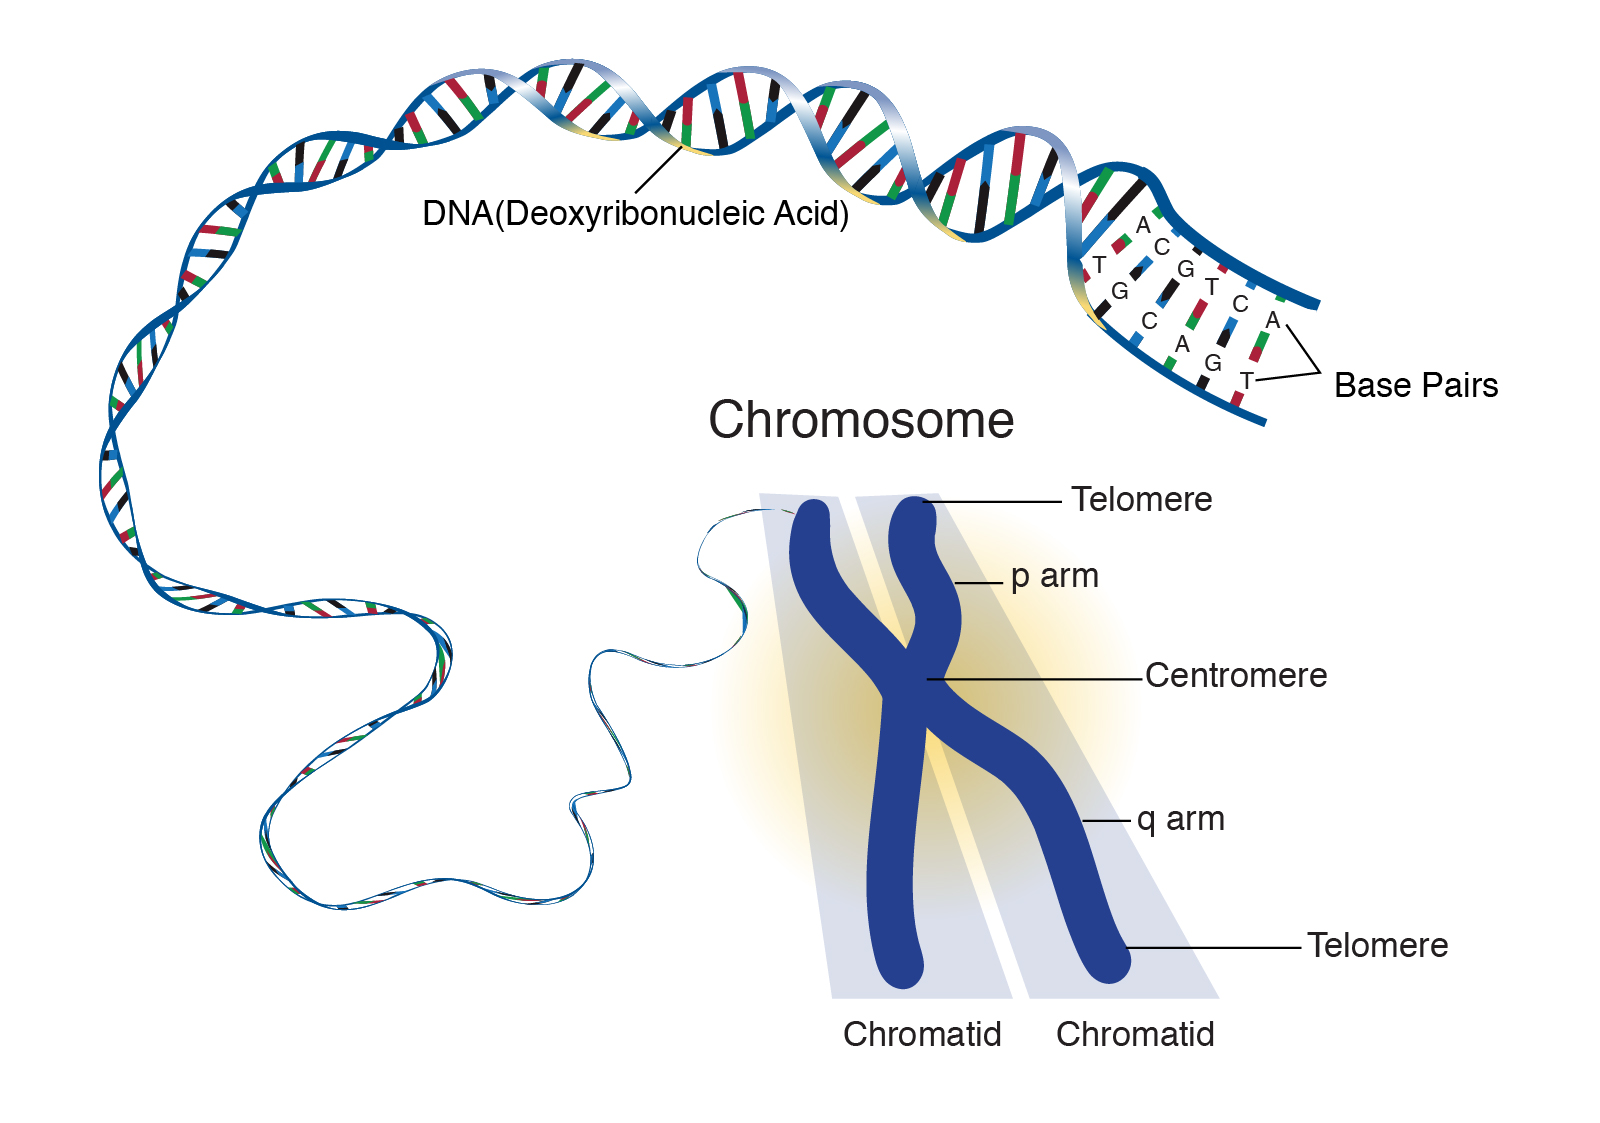
\includegraphics[width=200px]{./img/chromosome.jpg}
		\caption{Převzato z \cite{human_cell} a \cite{chromosome_structure}}
		\label{fig:chrmosome}
\end{figure}

\noindent
Uvnitř buňky je obsažen celý genom, který se ovšem nemusí projevit na povrchu buňky. Pokud se vlastnost, kterou gen přenáší, projeví na povrchu buňky označujeme to jako exprese genu (jeho sebevyjádření). Od toho se odvíjí i konkrétní názvosloví typu gen, receptor či molekula.


\section{HLA a non-HLA geny}
Human leucocyte antigen (HLA) je genetický systém, který je primárně zodpovědný za rozeznávání vlastního od cizorodého. Někdy je termín HLA zaměňován s MHC. MHC (Major histocompatibility complex) je souhrný termín pro všechny komplexy, kdy podskupinou jsou právě HLA (H - Human), který se vyskytuje u lidí. Stejně tak existuje DLA (D - Dog), který je pro psy. Z funkčního i biologického hlediska jde však u všech savců o stejnou skupinu genů. \cite{KIR_transplantace_jindra}
\\
\\
Přesná definice rozdílu mezi HLA a non-HLA geny neexistuje. Mimo jiné ani jejich rozdělení není v literatuře sjednocené. Jak je vidět na obrázku \ref{fig:hla_genome}, je možné geny rozdělit do tří tříd. V některé literatuře je možné nalézt označení non-HLA genů jako geny III.třídy, v jiné, že jsou to všechny geny III. třídy a některé geny třídy I. Tato práce bude terminologicky vycházet v označení gen za non-HLA či HLA z definice uvedené v \cite{imgt_hla_database}. Zjednodušeně tedy můžeme říci, že geny, které nejsou řazeny k HLA skupinám, jsou non-HLA. Je-li gen označen za non-HLA, neznamená to, že by neměl souvislost s funkcí imunitního systému. Naopak má, jen ne výlučně s HLA systémem. Non-HLA geny kódují produkty spojené s imunitními procesy. Mezi non-HLA geny mimo jiné patří MICA, MICB a KIR. \cite{imgt_hla_database}

\begin{figure}[H]		
		\centering
		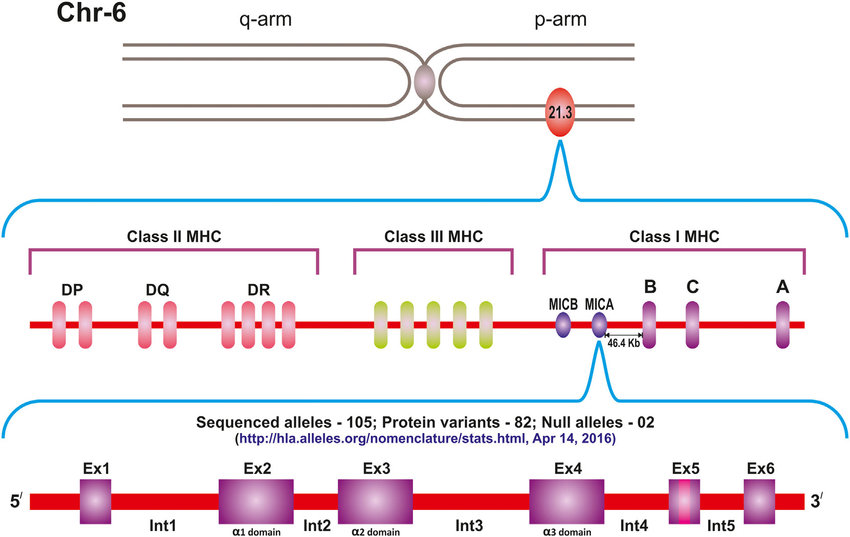
\includegraphics[width=300px]{./img/genom6_mica.jpg}
		\caption{Šestý chromozom zobrazující HLA(-A, -B, -C, -DR, -DQ, -DP) i non-HLA(MICA, MICB) geny. Protein vzniklý expresí genu je definován exony, které definují transkripci(přepis) do RNA. Introny při translaci(překladu) nehrají roli a často jsou sekvenovány jen exony. \cite{chromozome6_mica} 
		}
		\label{fig:hla_genome}
\end{figure}

\noindent
HLA a některé non-HLA geny se nacházejí na krátkém raménku 6. chromozomu, konkrétně 6p21.3, a zaujímají úsek přibližně jedné tisíciny genomu. Tento region je nejvíce komplexní a polymorfní v lidském genomu s více než 220 geny. Oproti tomu jedna ze skupin non-HLA genů, konkrétně KIR geny, se nachází na 19. chromozomu. Rozsáhlá diverzita těchto genů vznikala snahou eliminovat neustále se měnící spektrum patogenů. Produkty těchto genů na povrchu buňky významně ovlivňují odpověď na infekční choroby a výsledky buněčné či orgánové transplantace. \cite{imgt_hla_database}
\\
\\
Při určování shody dárce a pacienta se rozhoduje na základě shody alel u genů HLA -A, -B, -C, -DRB1, -DQB1. Díky velké diverzitě HLA genů je počet možných kombinací několik miliard. Některé kombinace genů se vyskytují na základě oblasti či národnosti častěji nebo mohou být naopak vzácné. HLA geny se obvykle dědí jako blok (cely haplotyp), avšak ve výjimečných případech může dojít k rekombinaci. Z tohoto důvodu je nejsnadnější nalézt shodu v pokrevním příbuzenstvu.
\\
\\
Jelikož každý jedinec má dvakrát geny na pozicích HLA -A, -B, -C, -DRB1 a -DQB1 (jednu pětici od otce, druhou pětici od matky), je maximální shoda 10/10 (shoda obou alel v lokusech) popř. DPB1 a shoda 12/12. Čím je shoda menší, tím větší je riziko nepřijetí štěpu. U nepříbuzných jedinců lze tolerovat shodu 9/10 či 8/10. \cite{Frycova_bakalarka} \cite{KIR_transplantace_jindra}
\\
\\
V posledních letech se objevuje Haploidentická transplantace, kdy je možné použít krvetvorné buňky příbuzného se shodou pouze jednoho haplotypu (5/10) například jedinec může využít transplantace od vlastního rodičů nebo sourozenců. Umožnuje to podávání chemoterapie pár dní po transplantaci, která zničí všechny buňky, které tělo nepřijme. Tímto způsobem může být celý proces transplantace výrazně urychlen, zejména v případech, kdy není čas hledat dárce v registrech \cite{haploidenticka_transplantace}

\subsection{Alela a gen}
Alelu můžeme definovat jako variantu genu s nepatrným rozdílem v sekvenci nukleotidů DNA oproti jiné alele stejného genu. Jinak řečeno, alely jsou varianty genu na molekulární úrovni. Geny se zpravidla vyskytují minimálně ve dvou formách (dvou alelách). Gen určuje výskyt nějakého znaku, například oči konkrétního živočicha budou mít barvu. Alela pak určuje, jaká barva to bude. Jinak řečeno, alela zajišťuje konkrétní fenotypový projev genu.
\\
\\
V případě genu KIR2DL1 mohou být jeho alely 0010101 a 0010102. Zápis genů tak, jak s nimi budeme pracovat, může vypadat způsobem zobrazeným v \ref{alela_gen_prikad}. 

\begin{equation}\begin{split} 
   \label{alela_gen_prikad}
   		>KIR:KIR00001\: KIR2DL1*0010101\: 14738\: bp \\
		GTTCGGGAGGTTGGATCTCAGACGTG...
\end{split}\end{equation}

\noindent 
Označení $KIR:KIR0001$ označuje pořadové číslo, kdy alela byla nalezena. Oproti tomu $KIR2DL1*0010101$ je označení genu podle jeho vlastnotí.
\\
\\
K zjištění konkrétních alelických variant se pro tzv. typizaci využívají sekvenační metody, typicky s polymerázovou řetězovou reakcí. 


\section{Natural killer a jeho receptory}
Natural killer buňky (NK buňky) jsou velké granulární lymfocyty vrozeného imunitního systému. V krevním oběhu lidského těla je jich možné nalézt $10-15 \%$. Klíčovou vlastností NK buněk je nejenom schopnost rozlišit poškozené buňky od zdravých, ale také poškozené buňky rychle a efektivně likvidovat. Poškozené buňky mohou být buňky infikované virem či buňky transfomované v nádorové. Na povrchu NK buňky se nachází receptory, které jsou zobrazeny na obrázku \ref{fig:NK_receptors}, regulující odpověď imunitního systému. Natural killer buňky oproti B- a T- lymfocytům (buňkám získané imunity) nemají antigenně specifické receptory. Jedním ze způsobů jak NK buňky rozpoznávají a zabíjejí poškozené buňky, je na základě interakce mezi KIR receptorem a HLA molekulou na povrchu zkoumané buňky (podrobněji viz sekce KIR). Stejně tak mohou zabíjet na základě receptoru NKG2D, který aktivuje cytoxickou reakci při setkání s ligandem MICA a MICB. Ligandem označujeme malou molekulu, která se váže na vazebné místo cílového proteinu(receptoru) a vyvolává fyziologickou odpověď, která může mít inhibiční či aktivační charakter. 
% https://www.khanacademy.org/science/biology/cell-signaling/mechanisms-of-cell-signaling/a/signal-perception
\begin{figure}[H]		
		\centering
		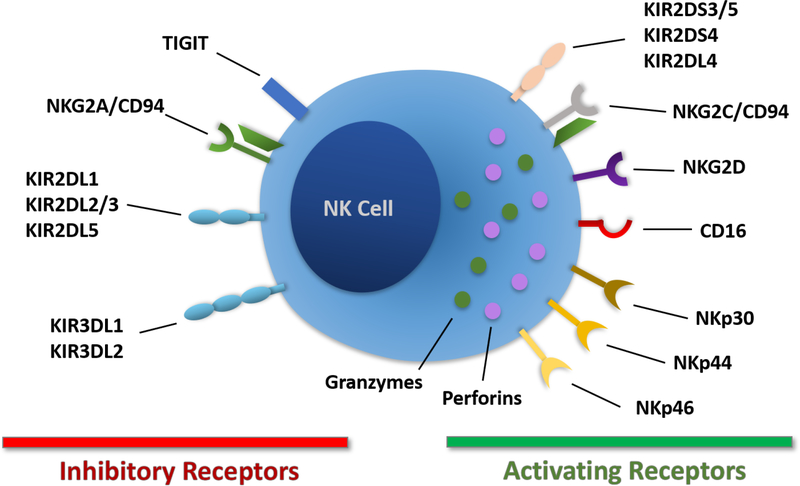
\includegraphics[width=300px]{./img/nk_receptory.jpg}
		\caption{Natural killer buňka a její receptory, rozděleny na aktivační a inhibiční.\cite{NK_receptors} }
		\label{fig:NK_receptors}
\end{figure}

\subsection{NKG2D receptor}
NKG2D je jeden z nejvýznamnějších aktivačních receptorů na NK buňce rozpoznávající především buněčný stres, který může spustit cytotoxicitu (schopnost ničit buňky), i když se na povrchu buňky nachází inhibiční HLA-I ligandy.  
\\
\\
Geny skupiny MICA a MICB jsou označovany jako class I chain-related gene. To znamená, že se běžně neřadí do I. třídy MHC. Takto označované geny mají souvislost s MHC I. třídy, ale na rozdíl od nich neváží peptidy. Oproti HLA genům, které mají svoje produkty na lymfocytech, se produkty MICA a MICB nachází na epitelových buňkách. Nejedná se tedy o standardní HLA geny, proto jsou v novějších zdrojích označovány jako non-HLA. Jejich expresí na povrch buňky jsou ligandy, které se váží na receptor NKG2D. Buňky s ligandy MICA a MICB se množí při nádorovém onemocnění, zanětu nebo pod vlivem různých forem buněčného stresu, a díky navázání na receptor může být spuštěna imunitní reakce. \cite{transfuzni_lekarstvi} \cite{MIC} \cite{NK_receptors} \cite{imgt_hla_database}


\subsection{KIR receptor}
Killer immunoglobulin-like receptor (KIR) je skupina genů řazených mezi non-HLA geny. Jejich zvláštností je fakt, že se nenachází na 6. chromozomu, ale na 19. a tak se dárci se schodnými HLA znaky nemusí schodovat v KIR znacích. Expresí KIR genů jsou receptory na povrchu natural killer buněk. Dnes je známo 15 genů a 2 pseudogeny rozlišující se na inhibiční a aktivační na základě cytoplasmatického ocásku a počtu imunoglobulínových domén. \citep{KIR_transplantace_jindra}

\begin{figure}[H]		
		\centering
		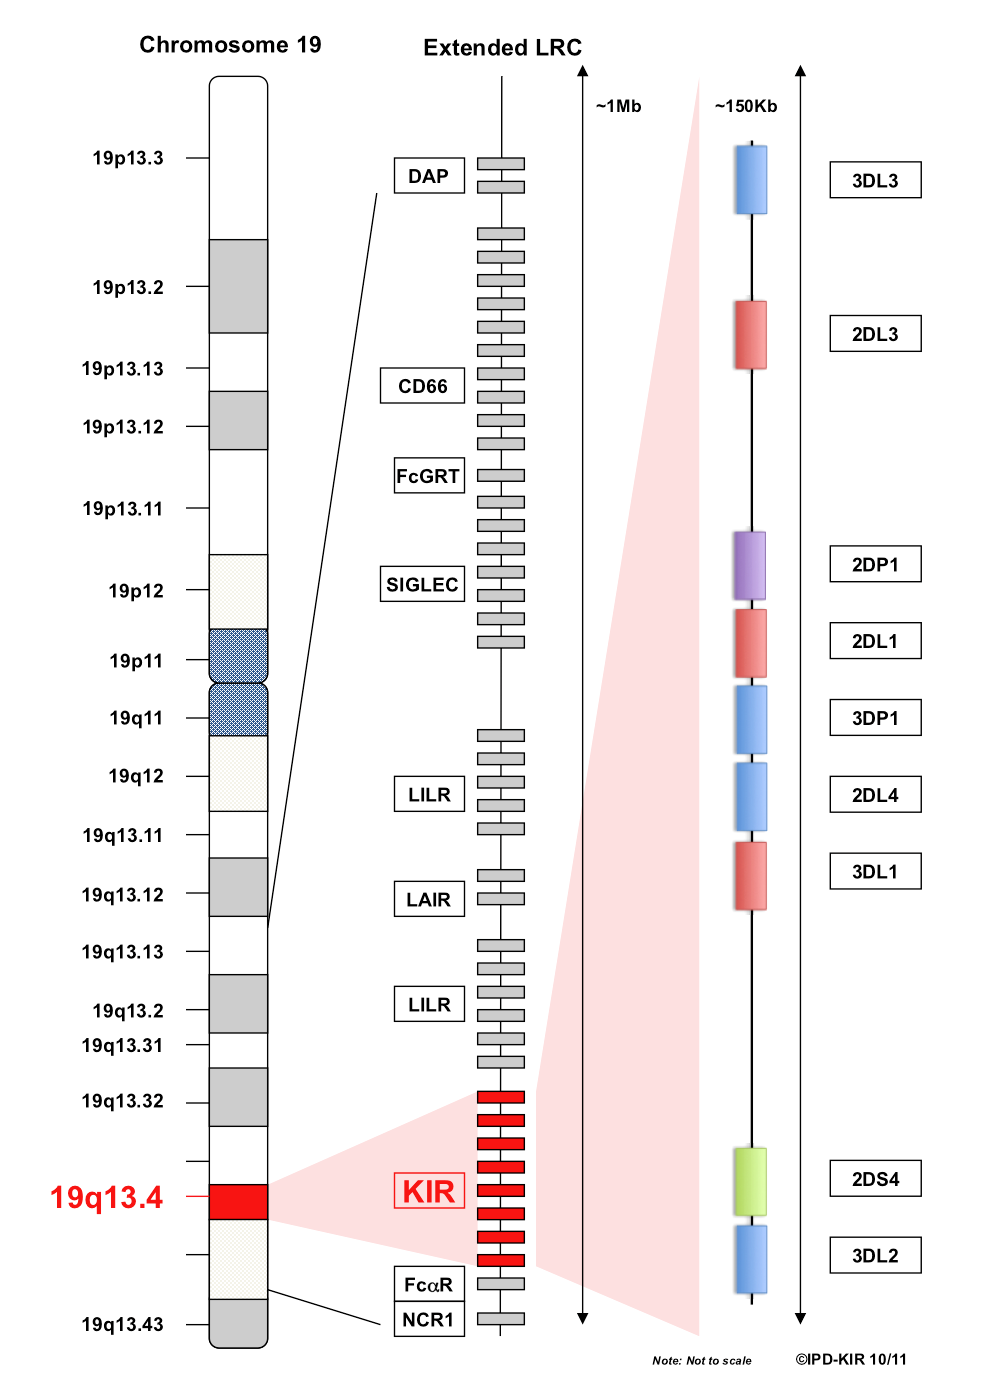
\includegraphics[width=250px]{./img/kir_pozice.png}
		\caption{KIR se nachází na 19. chromozomu v oblasti jménem leukocyte receptor complex (LRC). \cite{imgt_hla_database}}
		\label{fig:kir_position}
\end{figure}

\subsubsection{Nomenklatura KIR genů}
KIR geny (na obrázku \ref{fig:img_kir_nomenklatura}) se liší různou délkou cytoplasmatického ocásku (tail) a různým počtem imunoglobulin-like domén (lg-like). Na základě této rozmanitosti byla založena nomenklatura KIR genů, tedy jejich pojmenování. 
\\
\\
Jak je vidět na obrázku~\ref{fig:img_kir_nomenklatura}, cytoplasmatický ocásek může být dlouhý (long~-~L) nebo krátký (short~-~S). Je možné se setkat i s označením P, které slouží pro pseudogeny. Oproti tomu imunoglubulínové domény se mohou vyskytovat 2~(2D) nebo 3~(3D). Právě z těchto vlastností vychází základ pojmenování KIR genů. 
\\
\\
Příkladem může být KIR2DL1*010101, kde 2D označuje dvě imunoglubulinové domény, L značí dlouhý ocásek, 1 značí že je to první 2DL protein. Numerická definice alely je poté oddělena hvězdičkou. První tři čísla označují alely, které se liší v sekvencích jejich kódovaných proteinů, další dvě číslice se používají k rozlišení alel, které se liší synonymními rozdíly v kódující sekvenci. Konečné dvě cifry rozlišují alely na základě substituce v intronu, promotoru nebo jiné nekódující oblasti. \cite{imgt_hla_database}

\begin{figure}[H]		
		\centering
		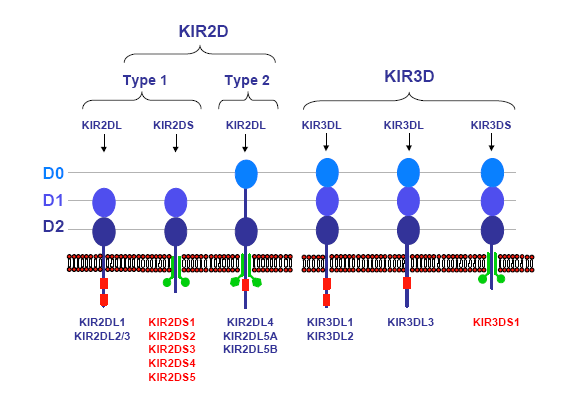
\includegraphics[width=\textwidth]{./img/KIR_nomenklatura.png}
		\caption{Nomenklatura KIR genů. \cite{KIR_transplantace_jindra}}
		\label{fig:img_kir_nomenklatura}
\end{figure}

\noindent
Další rozdělení KIR genů je na již výše zmíněné inhibiční a aktivační. Dle obrázků~\ref{fig:NK_receptors} a  \ref{fig:img_kir_nomenklatura} je možné si povšimnout detailu, že až na KIR2DL4 jsou aktivační KIR s krátkým ocáskem, zatímco inhibiční jsou s dlouhým ocáskem. 

\subsubsection{Aktivace NK buněk pomocí KIR}
Jak již bylo výše zmíněno, KIR receptory můžeme rozdělit na inhibiční a aktivační. O tom, zda dojde k aktivaci NK buňky, rozhoduje právě jejich rovnováha na zkoumané buňce. Obrázek \ref{fig:img_kir_ligand} ukazuje vazebné ligandy pro jednotlivé KIR receptory.  

\begin{figure}[H]		
		\centering
		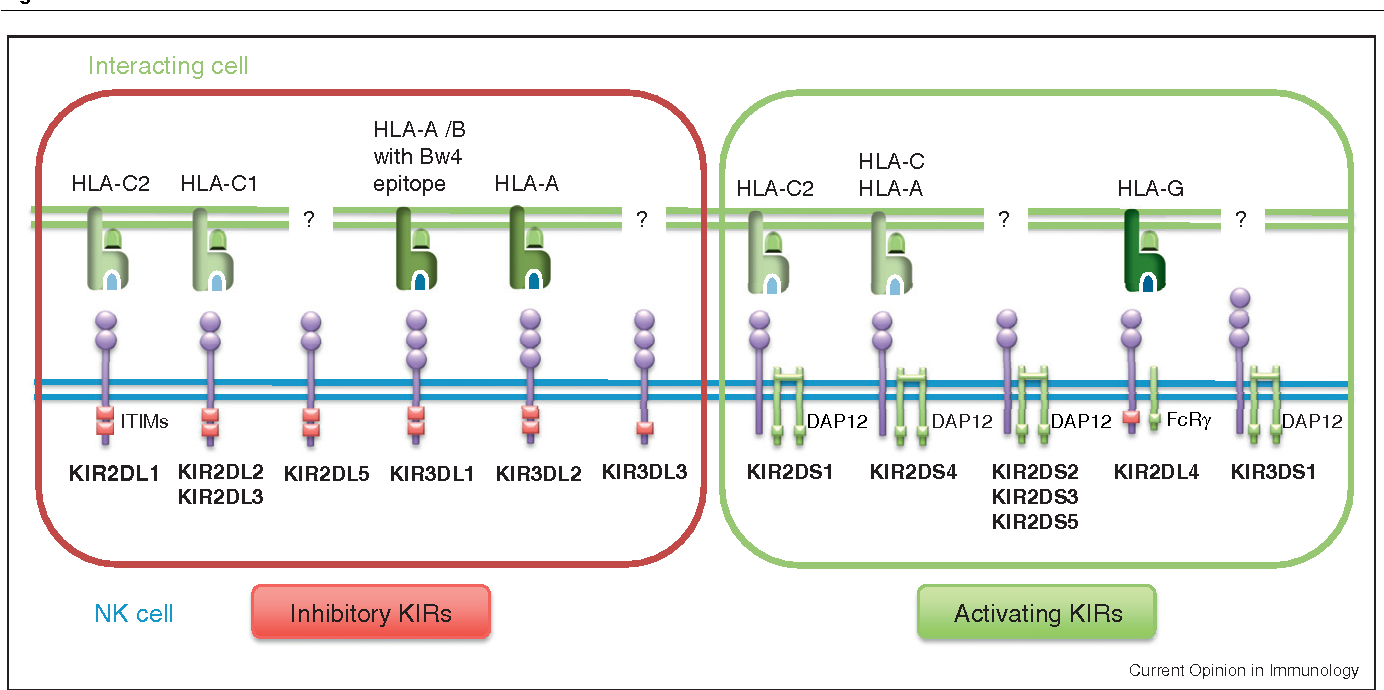
\includegraphics[width=\textwidth]{./img/KIR_nomenklatura2.png}
		\caption{KIR geny a jejich vazebné ligandy. Pokud je v obrázku ?, značí to, že pro daný receptor není znám vazebný ligand. \cite{KIR_img_nomenklatura}}
		\label{fig:img_kir_ligand}
\end{figure}

\noindent
NK buňky ustavičně prohledávají své okolí a testují přítomnost příslušných HLA ligand pro své KIR receptory. Pokud je příslušný HLA ligand přítomen, naváže se na NK buňku (\ref{fig:kir_princip} případ~1). Tímto systémem jsou ochráněny vlastní buňky. Pokud přítomen není, je spuštěna cytotoxická reakce a zkoumaná buňka je zničena.
\\
\\
Některé virem napadené buňky potlačují propsání HLA ligandu na povrch buňky a tím se brání cytotoxicitě vůči T lymfocytům. Zároveň se ale stávají citlivějšími na cytotoxicitu proti NK buňkám, jak je zobrazeno na obrázku \ref{fig:kir_princip} případ~3.
\begin{figure}[H]		
		\centering
		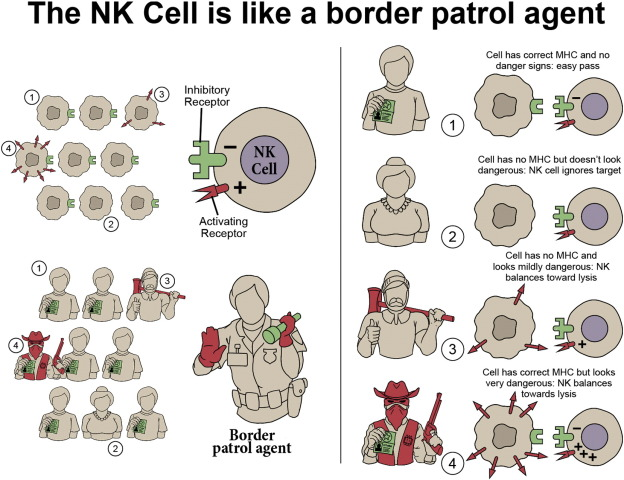
\includegraphics[width=\textwidth]{./img/NK_princip.jpg}
		\caption{Přirovnání fungování natural killer buňky k pasové kontrole. V pravé části jsou zobrazené případy, které mohou nastat, když natural killer buňka potká jinou buňku. V 1. případě je tělu vlastní zdravá buňka, kde se KIR receptor naváže na HLA ligand a k cytotoxitické reakci nedojde. Druhým případem je červená krvinka. K reakci NK buňky opět nedojde, protože na zkoumané buňce nepřevažují aktivační receptory. V 3. případě je to nádorová buňka, která schová HLA ligand, (může nastat po transplantaci kostní dřeně), a tím se "schová" proti T- lymfocytům. Avšak aktivační receptory převládají, a tak k cytotoxicitě dojde. Ve 4. příkladu je nádorová buňka nebo virem nakažená buňka (stresové ligandy). Aktivační receptory převládají, a tudíž k cytotoxické reakci dojde.\cite{KIR_img_princip}}
		\label{fig:kir_princip}
\end{figure}



\subsubsection{KIR genotyp a haplotyp}
KIR genotyp je vyjádření, jaké konkrétní KIR geny genom obsahuje. Genotyp je možné rozdělit na dvě části, takzvané haplotypy. Jeden haplotyp je od otce, druhý je od matky. Na základě kombinací všech genů je možné vytvořit velký počet KIR genotypů. Proto byl díky shromážděným haplotypům sestaven model, který toto množství mírně redukuje, přičemž samozřejmě nepokrývá všechny možné varianty. Haplotyp se rozděluje na dvě části, centromerickou a telomerickou v závislosti na tom, zda je blíže k centromeře či telomeře (viz. obrázek \ref{fig:chrmosome} pravá část). Jednotlivé části mezi sebou mohou být kombinovány. Centromerická i telomerická část může byt zařazena do jedné ze dvou skupin A či B na základě genů, které obsahuje (viz. obrázek \ref{fig:kir_haplotypy_ct} část A). Celý haplotyp je následně přiřazen do jedné ze dvou skupin podle kombinace centromerické a telomerické části. V případě, kdy jsou obě části A/A, je haplotyp označen za A, u ostatních kombinací (A/B, B/A, B/B) je haplotyp B (viz. obrázek \ref{fig:kir_haplotypy_ct} část B). Jiná definice pro rozdělení haplotypů uvádí, že skupina B musí obsahovat alespoň jeden z genů KIR2DL5, KIR2DS1, KIR2DS2, KIR2DS3, KIR2DS5 a KIR3DS1. Naopak skupina A neobsahuje ani jeden z těchto genů. Je třeba si zde uvědomit, že každý jedinec má 2 KIR haplotypy. \cite{KIR_haplotypy_ct}
\\
\\
\begin{figure}[H]		
		\centering
		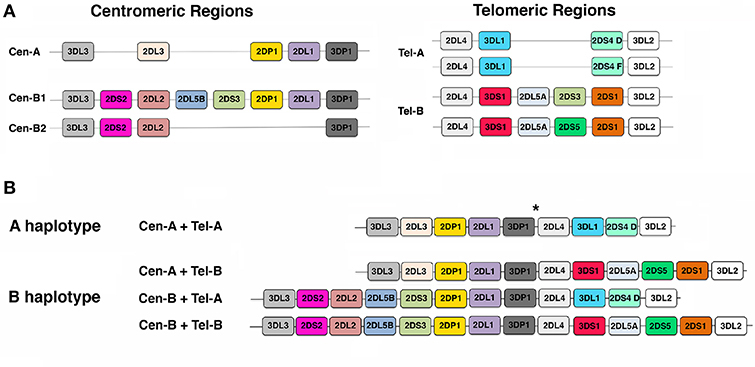
\includegraphics[width=\textwidth]{./img/KIR_haplotype.jpg}
		\caption{Rozdělení KIR genů na centromerickou a telomerickou část, pojmenování je na základě toho, zda je úsek blíže k centromeru nebo k telomeru (viz obrázek \ref{fig:chrmosome}). Je možné si zde povšimnout, že je možné některé geny najít jak v centromerické části, tak v telomerické části. Upraveno z \cite{KIR_haplotypy_ct}}
		\label{fig:kir_haplotypy_ct}
\end{figure}

\noindent
Podle některých studií zabývajících se vlivem KIR haplotypů na výsledky transplantace bylo zjištěno, že KIR haplotypy ovlivňují výsledky u akutní myeloidní leukemie či  lymfoblastické leukemie. Ve srovnání s haplotypem A měl haplotyp B, především jeho centromerická část, ochranný účinek před návratem nemoci a zároveň zvýšil pravděpodobnost přežití pacienta. Na základě této skutečnosti se mohou dárci řadit do tří skupin: best, better a neutral. Rozřazení do třídy se vyhodnocuje jako počet B a jejich umístění v centromerické oblasti či telomerické oblasti. Mimo jiné je možné se setkat s pojmem B-skóre. Toto číslo udává počet B, které se v daném haplotypu nachází. Best je definován B-skórem alespoň 2, přičemž dvě B se musejí nacházet v centromerické oblasti Cen-B/B a Tel-x/x. Better je definován B-skorém alespoň 2, aby nebyl haplotyp zařazen do best, musí být logicky alespoň jedna z centromerických oblastí A - Cen-A/x a Tel-B/x. Neutral je v případě jedné B části nebo žádné. \cite{KIR_haplotypy}
\\
\\
KIR geny se stejně jako HLA dědí jako celý blok. Jelikož HLA se nachází na 6. chromozomu a KIR na 19., tak shodní dárci v HLA znacích se jen menšinově shodují v KIR genech. V případě příbuzného dárce shodujícího se v HLA znacích je pouze 25 \% shodných také v KIR. \cite{KIR_haplotypy}

\begin{figure}[H]		
		\centering
		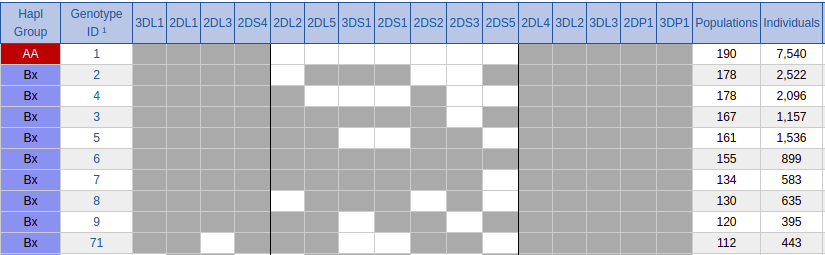
\includegraphics[width=\textwidth]{./img/KIR_haplotypy_priklad.png}
		\caption{Deset nejčastějších KIR haplotypů. Šedý obdélník značí přítomnost genu, bílý jeho nepřítomnost. \cite{kir_genotypes_10}}
		\label{fig:kir_haplotypy_10}
\end{figure}
 

\chapter{Sekvenační metody získávání DNA dat}
Po pojmem sekvence DNA se skrývá posloupnost písmen představujících primární strukturu reálné nebo hypotetické molekuly či vlákna DNA, které nese nějakou informaci. Jednotlivá písmena jsou označována jako nukleotidy nebo nukleové báze. Nukleové báze mohou být A~-~adenin, C~-~cytosin, G~-~guanin a T - thymin. \cite{genome_gov}
\\
\\
\noindent
Příkladem může být následující úsek sekvence na základě obrázku \ref{fig:chrmosome} 
\begin{align}
   \label{sekvence_prikad} ACGTCA
\end{align}

\noindent
\textbf{Sekvenování DNA}, někdy pouze sekvenování, jsou biochemické metody, kterými se zjišťuje pořadí nukleotidů (A, C, G, T) v sekvenci DNA. Díky tomu je možné zjistit typizaci konkrétního člověka. Sekvenační metody se liší zejména délkou řetězce, kterou dokáží zpracovat, cenou a rychlostí sekvenace. Pro porovnání, sekvenování celého genomu Sangerovo metodou by stálo několik milionů dolarů a trvalo zrhuba 10 let. Při použití dnešních metod by cena byla zhruba tisíc dolarů. Většina sekvenačních metod využívá vlasnosti přitahování báze do páru pouze jednou konkrétní bází. To znamená že se adenin vždy páruje s thyminem a cytosin se vždy páruje s guaninem. Z těchto párů vzniká již známá dvojitá šroubovice DNA. V praxi není neobvyklé, že se sekvenuje jen kónkrétní kus DNA, který je zrovna výzkumně či jinak potřebný. Největším problémem u sekvenování je, že úseky DNA vzniklé ze sekvenátoru (označovány jako ready) jsou jen kousky, které je třeba poskládat zpět. K tomu slouží zarovnávání. \cite{sekvenovani_ziva} 


\section{Sanger sequencing}
Sanger sekvenování využívá možnosti namnožení řetězce díky vzájemnému přitahování konkrétních bází. V prvním kroku replikace jsou nastříhané řetězce rozděleny na dvě vlákna. Lze si představit, že tato dvě oddělená vlákna jsou umístěna do směsi, kde plavou jednotlivé nukleotidy spolu s upravenými nukleotidy, které nesou specifickou fluorescenční barvu a na které není možné nic navázat. Následně za pomoci střídaní teploty volně plující nukleotidy tvoří postupně páry s řetězcem, který chceme namnožit. Pokud se povede celý řetězec namnožit, je odtržen a může se dále množit. Postupně ale bude docházet k navazování nukleotidů s fluorescenční barvou. Tím se vytvoří několik různě dlouhých sekvencí zakončených označeným nukleotidem. Podle jeho barvy je možné poznat o jaký nukleotid se jedná. Následně jsou za pomoci elektorforézy seřazeny v gelu podle délky. Elektroforéza rozděluje různě dlouhé sekvence na základně odlišnosti pohybu v elektrickém poli. Kratší doputují dále než delší. Pomocí Sanger metody je možné sekvenovat řetěce dlouhé až 1000 bází.   

\begin{figure}[H]		
		\centering
		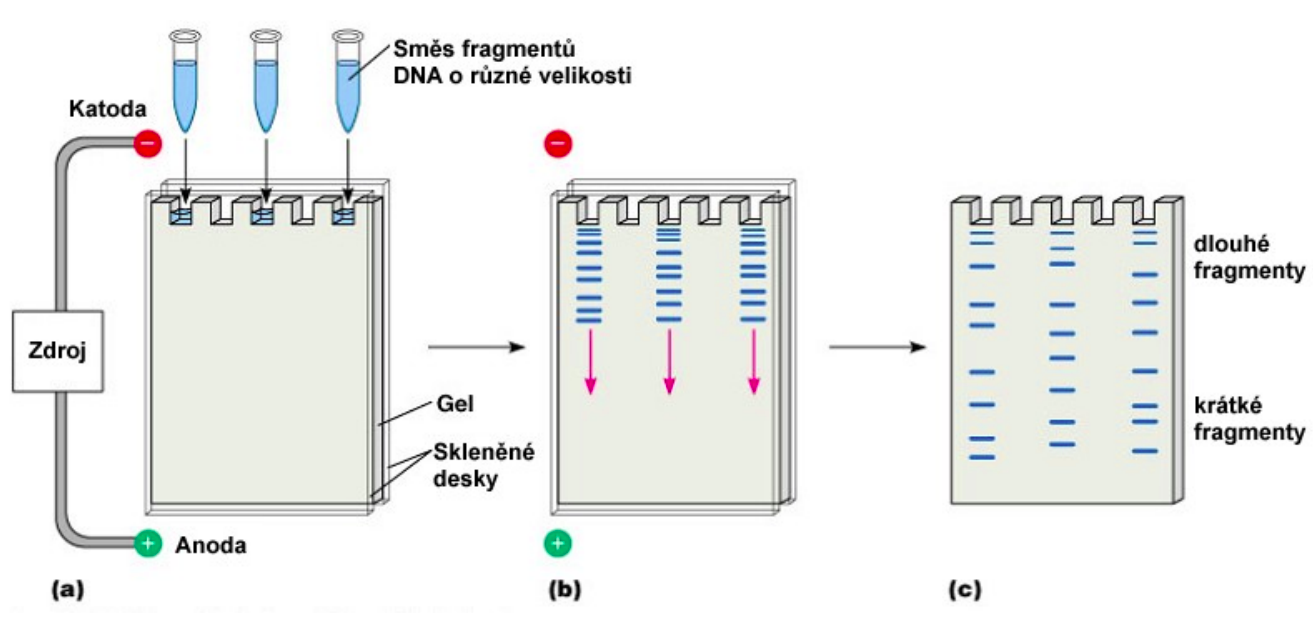
\includegraphics[width=\textwidth]{./img/elektroforeza.png}
		\caption{Elektroforéza. \cite{elektroforeza_img}}
		\label{fig:elektroforeza}
\end{figure}
 
\section{NGS next-generation sekvenování}
Next-generation sekvenování, někdy označováno jako metody druhé generace, je v porovnání se Sanger sekvenováním rychlejší a levnější, na druhou stranu, ale dokáže zpracovávat jen řetězce dlouhé 100 až 500 bází, má menší přesnost a častěji chybuje. Jeho rychlost spočívá především ve schopnosti detekovat přidávání bází jednu po druhé a zároveň sekvenovat tisíce až miliony rozdílných molekul DNA najednou. 
\\
\\
Všechny tyto metody si předpřipraví řetězce nastříháním DNA na krátké části a připevněním takzvaného adaptéru na jejich konec. Adaptér je krátká molekula DNA, která slouží k uchycení sekvenovaného úseku na pevný povrch. Řetězce DNA jsou namnoženy, díky čemuž vznikají klastry identických molekul koncentrovaných v jednom místě. Díky tomu je posílen signál, který by z pouhé jedné molekuly nebyl dostatečně silný. Tento signál je zachycen kamerou. Jeden z důvodů popularity NGS metod jsou i cenově dostupné stolní sekvenátory.
 
\subsection{Single-end, paired-end a mate-pair}
Single-end je sekvenování pouze jednoho konce molekuly. Nevýhoda tohoto způsobu se projevuje především na krátkých readech, kde se zvyšuje problém jejich správného umístění. Oproti tomu v případě paired-end se sekvenuje z obou konců daného úseku. Vzniklé dva ready jsou označeny a zárověň je známá jejich vzdálenost, která se pohybuje od 200 do 400 bp (base pair). Mate-pair je v podstatě paired-end s tím rozdílem, že je mezi ready větší vzdálenosti od 2 do 5 kb (kilobase) - takže přibližně 2000 - 5000 bp. \cite{illumina}  

\begin{figure}[H]		
		\centering
		
\includegraphics[width=200px]{./img/single_end_pair_end_reads_yourgenome.png}
		\caption{Single-end a paired-end read. \cite{your_genome} }
		\label{fig:single_end_paired_end}
\end{figure} 
 

\subsection{454 sekvenování a Ion Torrent}
Pomocí 454 sekvenování je možné analyzovat více než milion molekul DNA najednou a délka každé jednotlivé sekvence se pohybuje okolo 700 až 1000 bází. V prvním kroku sekvenování je fragment DNA přichycen na malou "kuličku" \space na jejímž povrchu se postupně namnoží až kuličku zcela pokryjí identické fragmenty DNA. Následuje vložení kuličky i s DNA do jedné z milionů komůrek na destičce s reakční směsí. Postup je znázorněn na obrázku \ref{fig:sekvenovani_454}. V určitém momentu je do této směsi přidán vždy jen jeden typ báze. Mezi jednotlivými fázemi přidávání určité báze jsou přebytečné nukleotidy z předešlého kroku odstraněny. To znamená, že v reakční směsi je vždy jen jeden typ nukleotidů. Během vložení každé nové báze do rostoucího řetězce DNA je uvolněna molekula zvaná pyrofosfát, která spustí několik chemických reakcí. V poslední fázi enzym luciferáza vydá světelný záblesk, který je možné zachytit citlivou kamerou. Tento postup se nazývá pyrosekvenování. V případě, kdy je do řetězce přidáno několik stejných bází za sebou, například gen obsahuje podřetězec AAA, je vyzářeno, v tomto případě třikrát více světla než v případě jedné přiřazené báze. Kamera snímá celou destičku a na základě toho, která komůrka se rozsvítí, pozná, kde proběhlo přidání báze. Intenzita světla pak určuje kolik bází bylo přidáno najednou. 


\begin{figure}[H]		
		\centering
		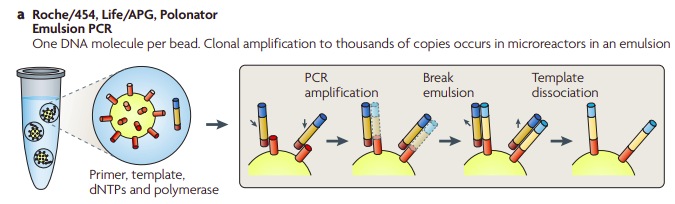
\includegraphics[width=300px]{./img/sekvenace_454_1.png}
		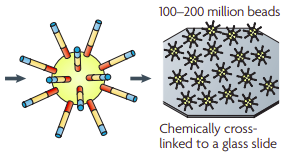
\includegraphics[width=150px]{./img/sekvenace_454_2.png}
		\caption{454 sekvenování. \cite{ngs_merzker}}
		\label{fig:sekvenovani_454}
\end{figure}

\noindent
Sekvenování Ion Torrent funguje na podobném principu sekvenování s tím rozdílem, že místo světla se měří změna pH v reakční směsi. Podle intenzity změny pH lze pak poznat kolik nukleotidů bylo přidáno do rostoucího řetězce.
\\
\\
Hlavní slabinou těchto dvou metod je značná chybovost při přidání mnoha stejných nukleotidů do řetězce za sebou. Například při přidání 10 A, nebude možné jednoznačně určit, zda se jedná o 10 A nebo 9 A.


\subsection{Illumina}
Při sekvenování pomocí Illumina jsou páry dvoušrobovice rozděleny na dva řetězce. Jednotlivé řetezce jsou následně přichyceny na malou destičku pomocí adaptéru. Každý řetězec se následně opakovaně množí až na destičce vznikne několik shluků. Přidání jedné molekuly ke druhé probíhá obdobně jako u Sanger sekvenování. Každý shluk tvoří jednu skupinu vzájemně identických řetězců. Mezi volné nukleotidy jsou opět zahrnuty nukleotidy označeny fluorescenční barvou, za které nelze nic navázat. Oproti Sangerovu sekvenování je ale tato blokace vratná a po přečtení citlivou kamerou dojde k odstranění blokující části molekuly. Počítač si pak následně zpětně spočítá, o který nukleotid se jednalo (na základě barvy). \cite{illumina} \cite{sekvenovani_ziva} 


\subsection{SOLiD}
SOLiD (Sequencing by Oligonucleotide Ligation and Detection) se spoléhá na enzym ligáza. Enzym je bílkovina, která určuje rychlost chemických reakcí. Enzym ligáza konkrétně umožňuje připojení jednořetězcových molekul k stávajícím řetězcům. K řetězcům jsou přidávány takzvané sondy, což jsou kousky DNA. Sondy začínají všemi možnými dvojkombinacemi čtyř základních nukleotidů. V součtu je 16 sond. Na každé sondě je jedna ze čtyř flurescenčních barev. V jednotlivých krocích jsou sondy připojeny k rostoucímu řetězci. Následně je přečtena fluorescenční barva, která je pak odstraněna, a může se tak navázat další sonda. Z výsledného signálu lze pak odvodit sekvenci DNA.


\section{Metody třetí generace}
Velkým rozdílem oproti druhé generaci je, že DNA řetězec není před sekvenování namnožen a je čten pouze z jedné původní molekuly. Existuje například PacBio od Pacific Bioscience, který k detekci využívá fluorescenčně značené nukleotidy. Díky jeho vysoké citlovosti je možné v reálnám čase zachytit přidání i jediného nukleotidu do jediného řetězce DNA. Dalším zástupcem těchto metod je Oxford Nanapore, jehož výhodou je jeho velikost. Oxford využívá odlišného tvaru bází. Obě metody jsou schopné přečíst přes 10 tisíc bází v rámci jedné analyzované molekuly DNA. 


\chapter{Analýza dostupných bioinformatických nástrojů pro zpracování NGS dat}
NGS metody snižují náklady a zrychlují proces sekvenování za cenu kratších readů a menší přesnosti, což vedlo k mnoha bioinformatickým výzvám jako je vytvoření nástrojů pro analýzu readů. Nástroje je možné mezi sebou porovnat pomocí reálných nebo simulovaných dat. Přestože je validace na reálných datech nezbytná, skutečné hodnoty na kterých jsou data založena jsou obvykle neznámé, což komplikuje jejich použití pro posouzení přesnosti (tj. jak blízko je odhadovaná hodnota ke skutečné hodnotě). Díky tomu je simulování dat čím dál více populární pro hodnocení, validaci či nastavování optimálních parametrů nástroje. \cite{simulation_read}


\section{Simulační nástroje pro generování syntetických readů}
Dále uvedené nástroje byly vybrány na základě těchto parametrů: simulování DNA, udržitelnost a volná dostupnost. Následující informace vychází z článku \cite{simulation_read}, pokud nebude uvedeno jinak.
\\
\\
Většina simulátorů NGS vyžaduje referenční sekvenci, ze které budou generovat ready. Tato referenční sekvence může být konkrétní genomická oblast, více zřetězených genomických oblastí, chromozom či celý genom. Některé simulátory vytváří zarovnání readů přímo do referenčního souboru (soubory SAM/BAM). Při používání simulátorů může být pro uživatele obtížné se rozhodnout, kterou konkrétní hodnotu pro daný parametr určit nebo který vlastní profil vytvořit, proto některé simulátory poskytují výchozí profily. Jedním z nich může být i generování chyb či modelu kvality. Nástroje jako jsou ART nebo SInC generují tyto profily na základě extrahovaných modelů ze skutečných dat. Nejčastější chyby jsou způsobeny substitucí, vložením či smazáním (INDEL - insert-deletion).


\begin{figure}[H]		
		\centering
		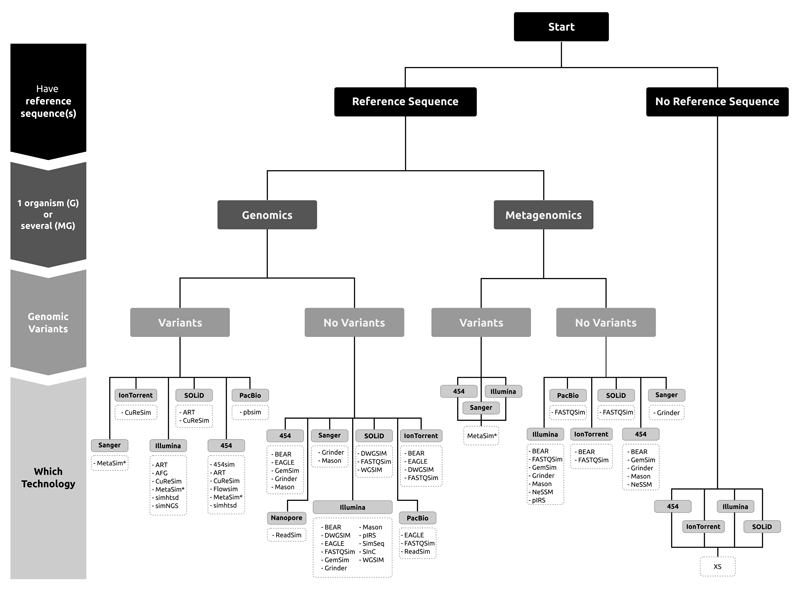
\includegraphics[width=1\textwidth]{./img/read_simulators.jpg}
		\caption{Strom pro usnadnění výběru generátoru syntetických readů. \cite{simulation_read}}
		\label{fig:read_simulators}
\end{figure}

\noindent
Data získaná z FN Plzeň/BC LF UK Plzeň jsou primárně sekvenována nástrojem Illumina, proto je podle \cite{simulation_read} na výběr z ART, AFG, CuReSim, Flowsim, MetaSim, simhtsd a simNGS. U simulátoru AFG je třeba chybové profily definovat ručně, CuReSim a MetaSim nejsou open source, simhtsd podporuje jen operační systém Linux, simNGS podporuje jen operační systémi Linux a MacOS. Proto byl vybrán simulační nástroj ART který podporuje operační systémy Linux, Windows a MacOS. Tento nástroj dále generuje podle chybových profilů a profilů kvality, které byly vytvořeny pomocí extrakce chyb získaných ze skutečných dat. 

\subsection{ART}
ART (next-generation sequencing read simulator) je sada simulačních nástrojů, které generují syntetické ready, jako kdyby byly získány sekvenováním pomocí NGS. Nástroj ART dokáže simulovat single-end a paired-end ready ze sekvenátorů Illumina, 454 společnosti Roch a SOLid od společnosti Applied biosystém. Ready vytvořené nástrojem ART, jsou používány pro testování a analýzu nástrojů zpracovávajících právě NGS sekvence, jako například nástroje Bowtie (zarovnávání). Při použítí nástroje ART je vstupním souborem sekvence genů, na základě kterých jsou vygenerovány ready. \cite{art}
\\
\\
Illumina je sekvenování založené na vratném umístění báze označené barvou do rostoucího řetězce. Jeho nejčastější chybou je substituce. Pravděpodobnost chyby substituce je určená na základě skóre kvality dané báze, které je závislé na pozici v rostoucím řetězci. Průměrné skóre kvality klesá v závislosti na zvyšování pozice báze. ART simuluje substituční chybu na základě zvyšování kvality báze a modelu pravděpodobnosti chyby získaného z reálných datasetů. INDEL chyba je simulována jen na základě modelu z reálných dat a u Illuminy se vyskytuje jen zřídka. Pro paired-end simulaci využívá ART dvou rozdílných skóre kvality pro každý pár readů jiný. 
\\
\\
ART je implementován v jazyce C++ a je dostupný s licencí GPL verze~3 pro operační systémy Linux, MacOs a Windows. Je možné ho použít i jako C++ package. Pro jeho spuštění je nutné mít nainstalovaný compilator GNU g++ 4.0 nebo vyšší a knihovnu GNU gsl. Výstupy se čtou ve formátu FASTQ a zarovnání ve formátu ALN. ART může generovat zarovánávání také ve formátu SAM nebo UCS BED. Paired end ready jsou označeny stejným názvem souboru s 1 či 2 na jeho konci.

\section{Nástroje pro zarovnávání readů}
Zarovnávání bývá prvním krokem v mnoha genomických pipelinách. Často je to jejich nejpomalejší část, protože pro každý read musí zarovnávač vyřešit obtížný výpočetní problém. Určit pravděpodobné umístění v referenčním genomu. 
V současnosti je na výběr více než 90 nástrojů pro zarovnávání NGS readů.
Nástoje jsou mezi sebou obvykle porovnávany na základě přesnosti a rychlost mapování. V článku \cite{ngs_alignment_software} bylo porovnáno 5 nástrojů pro zarovnávání DNA readů.  Nástroj STAR měl narozdíl od ostatních nástrojů menší přesnost, nástroj segemehl byl zase náročný na paměť (podle článku až 70 GB), což se na stolním počítači těžko dosahuje. Ze zbývajících nástojů byl vybrán nástroj Bowtie2 díky jeho rychlosti v porovnání s nástojem BWA, která vzhledem k množství požadovaných zarovnání bude přínosem.  

\begin{figure}[H]		
		\centering
		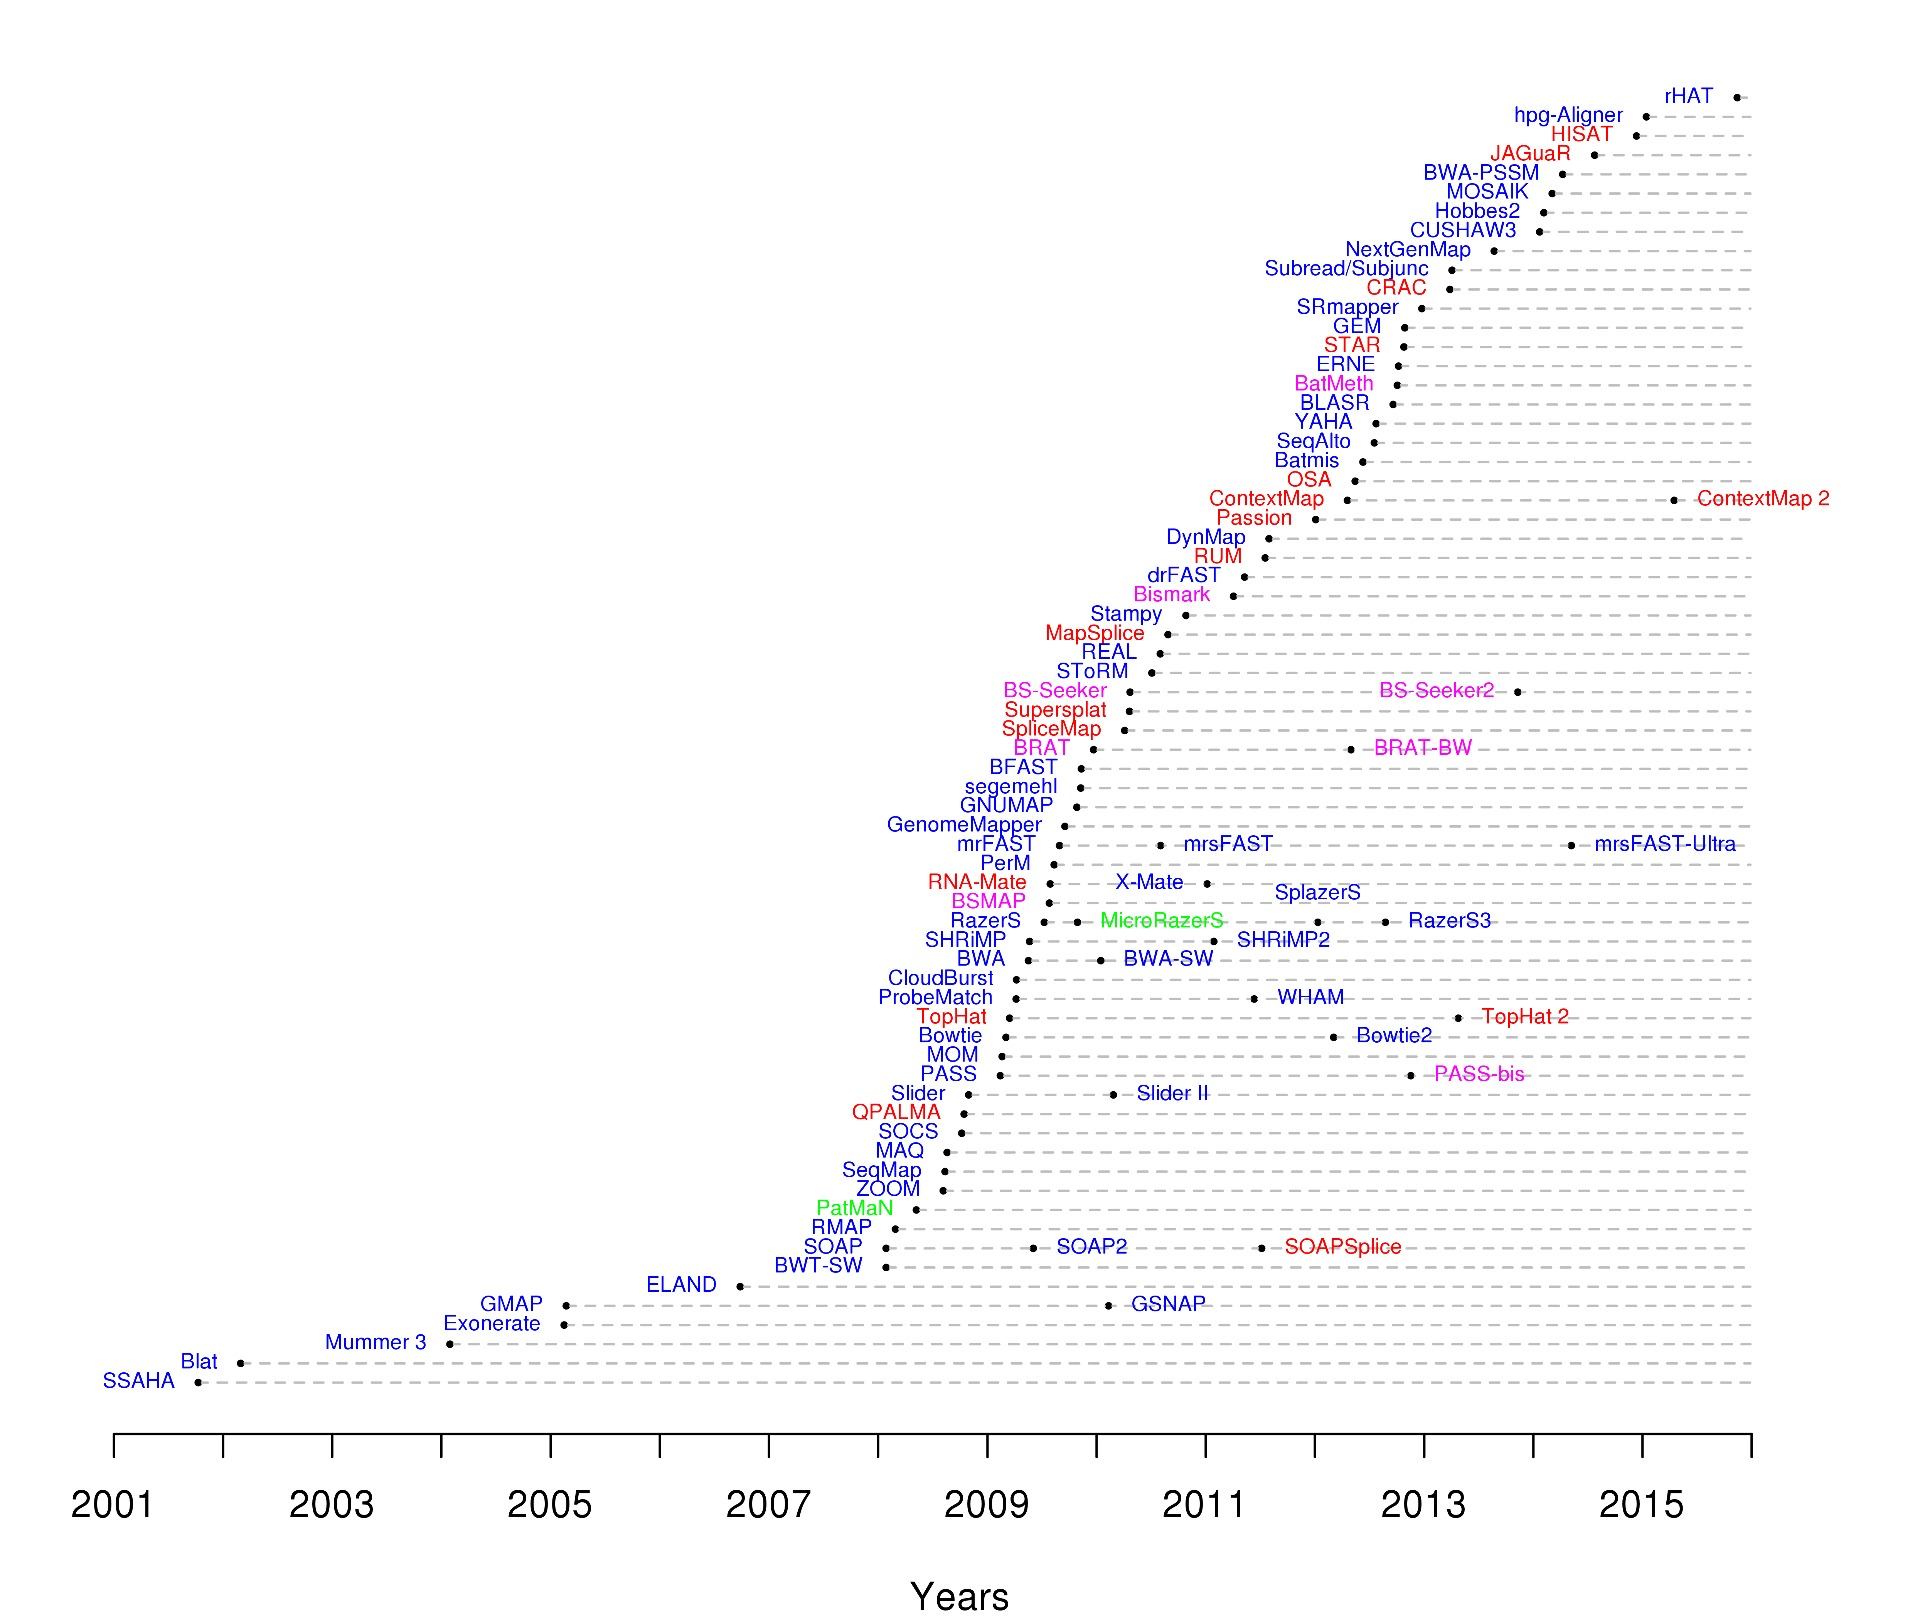
\includegraphics[width=1\textwidth]{./img/ngs_read_mappers.jpeg}
		\caption{Nástoje pro zarovnávání NGS readů. \cite{ngs_alignment_software}}
		\label{fig:align_tools}
\end{figure}

\subsection{Bowtie2}
Bowtie2 je rychlý a paměťově efektivní nástroj pro zarovnávání krátkých sekvencí DNA na velké genomy. Bowtie2 je schopný zarovnat více než 25 milionů readů dlouhých 35 bp za hodinu (při běhu na jednom CPU) pro lidský genom s malým využím paměti. Bowtie2 využívá FM indexaci s Burrows-Wheeler transformací (BWT) a přidává k ní backtracking pro sledování nekonzistence. Novější verze Bowtie2 by měla být oproti Bowtie1 citlivější a rychlejší na delší ready než je 50 nukleotidů, a navíc je oproti první verzi schopná se vypořádat z chybami vložení či smazání báze způsobené sekvenováním. Na lidský genom potřebuje Bowtie2 3.2 gigabajtů RAM. Nástroj bowtie je implementovaný v jazyce C++ s použitím knihovny SeqAn a je open source. Podporuje standardní vstupní formáty FASTQ a FASTA.  Výstupní zárovnání z Bowtie je ve formátu SAM, což umožňuje návaznost s dalšími nástroji jako je třeba SAMtools. Zbytek kapitoly shrnuje poznatky z článků \cite{bowtie} a \cite{bowtie2}, pokud není uvedeno jinak.   
\\
\\
Mnoho zarovnávačů používá indexy k rychlému snižování kandidátů pro umístění zarovnávaného readu. Bowtie permanentní indexy referenčních genů a lze je tak použít napříč běhy. Algoritmus FM indexu obvykle funguje na vyhledání přesně shody. V případě hledání umístění readů na referenční gen není toto řešení použitelné, protože ready mohou obsahovat chyby vzniklé sekvenováním, případně genové mutace. Proto Bowtie každé zarovnání zakládá na kvalitě znaku báze v daném readu. Bowtie postupně vytváří dlouhý sufix. Pokud se sufix nevyskytuje v textu, pak se může algoritmus vrátit a v již vytvořeném sufixu nahradit bázi za jinou. Dále pokračuje obdobným způsobem. Tento způsob změny báze je dále označován jako backtracking. Pokud by měl algoritmus na výběr substituovat za více bází, vybere tu s nejnižší kvalitou znaku v readu. Protože algoritmus Bowtie v základu bere první přijatelné řešení, je možné, že jeho nalezené řešení není to nejlepší. Pro nalezení toho nejlepšího řešení je třeba použít přepínač $--best$, jehož funkčnost je ale na úkor rychlosti, která může být 2x či 3x nižší. Bohužel nemůže být tento přepínač použit u paired-end readů. Zároveň je možné nastavit maximální počet nahrazených bází v readu. \cite{bowtie}
\\
\\
V případě, že backtracking mechanismus není úspěšný, může docházet k jeho nadměrnému výskytu. Bowtie2 se tento jev snaží zmírnit dvojím indexováním. První index obsahuje BWT genomu a je označován jako dopředný index. Druhý obsahuje opět BWT genomu, ale se znaky v sekvenci v opačném pořadí, označovaný jako zrcadlový index. Read je pak v půlce rozdělen na dvě části a jejich zarovnávání probíhá odděleně tak, že je vždy backtracking povolen jen v dané části, která je zrovna zarovnávána. Pravá část je zarovnáváná podle dopředného indexu a levá část je zarovnávána podle zrcadlového indexu. Předchozí algoritmus funguje dobře pouze v případě, kdy reference nebo read neobsahují mezery (báze chybí nebo naopak přebývá). Proto byl algoritmus rozšířen, jak je popsáno dále.

\begin{figure}[H]		
		\centering
		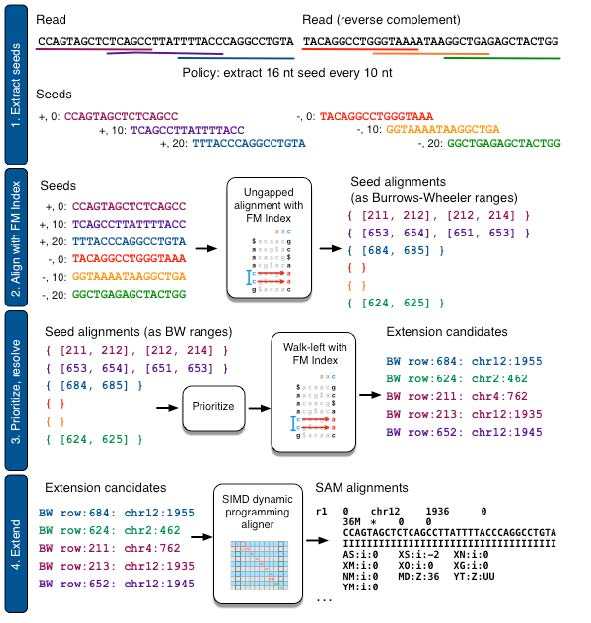
\includegraphics[width=1\textwidth]{./img/bowtie2_postup.png}
		\caption{Algoritmus zarovnání readů s mezerami. \cite{bowtie2}}
		\label{fig:bowtie_postup}
\end{figure}


\noindent
Pro každý read
\begin{enumerate}
	\item Extrahování seedu z readů (seedy tak představují části readu). 
	\item Seedy jsou zarovnány na referenci v bezmezerovém modelu za pomocí full-text minute indexu. Čísla v závorkách značí rozsah řádků v Burrows Wheeler matici, kam byl seed zarovnán.
	\item Seedy jsou seřazeny podle offsetu na referenčním genomu. 
	\item Ready jsou zarovnány. Díky předchozím krokům je značně omezen prostor, kam mohou být zarovnány. Pro zvýšení výkonu je použito SIMD (accelerated dynamic programming).
\end{enumerate}
  

\subsection{Burrows-Wheeler transformace}
Burrows-Wheelerova transformace (BWT) je reverzibilní permutace řetězců v textu. Původně byla používána pro kompresi dat. Indexace založená na BWT umožňuje efektivní vyhledávání ve velkém textu s malou paměťovou náročností. 
\\
\\
BW transformace řetězce T, $BWT(T)$, je zobrazena na obrázku \ref{fig:bw_transform_1}. Znak~$\$$ je připojen na konec řetězce a zároveň musí platit, že se tento znak v řetězci nevyskytuje. Burrows-Wheeler matice řetězce T je konstruovaná jako všechny cyklické rotace řetězce T, které byly seřazeny podle abecedy, znak \$ je řazen na začátek abecedy. Výstup, BWT(T) pak představuje poslední sloupec matice. Tento řetězec má stejnou délku jako původní řetězec T. \cite{bowtie} 

\begin{figure}[H]		
		\centering
		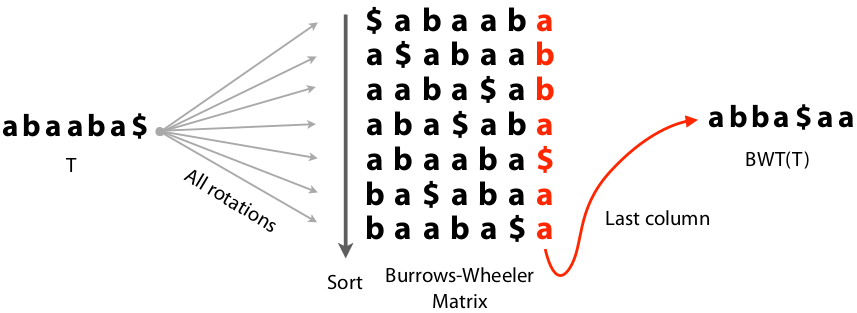
\includegraphics[width=.8\textwidth]{./img/BWT_1.png}
		\caption{Burrows-Wheeler transformace řetězce T. \cite{bw_transform}}
		\label{fig:bw_transform_1}
\end{figure}

\noindent
Burrows-Wheeler matice má vlastnost, která se nazývá last first mapping (LF). To znamená, že i-tý výskyt znaku X v prvním sloupci je i-tý výskyt znaku X v posledním sloupci. V případě přidání indexu do řetězce T je toto pravidlo pro znak $a$ zobrazeno na obrázku \ref{fig:bw_transform_lf}. Obdobně to platí i pro ostatní znaky v řetězci.

\begin{align}
   \label{rerezec_t} T - a_0 \: b_0 \: a_1 \: a_2 \: b_1 \: a_3 \: \$
\end{align}



\begin{figure}[H]		
		\centering
		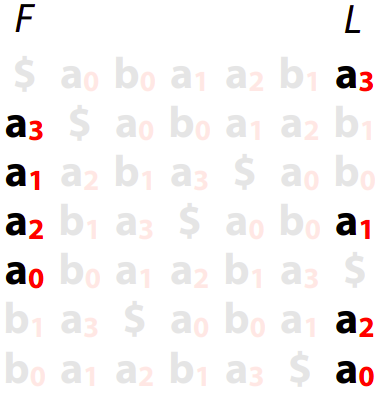
\includegraphics[width=100px]{./img/BWT_2.png}
		\caption{Burrows-Wheeler transformace last first mapping (LF). \cite{bw_transform}}
		\label{fig:bw_transform_lf}
\end{figure}

\noindent
Zpětné získání řetězce je znázorněno na obrázku \ref{fig:bw_transform_inverse}. L sloupec je řetězec, který je výstupem BW transformace. F sloupec, je na základě L sloupce, snadné odvodit. Jelikož platí pravidlo, že počet jednotlivých znaků je stejný, stačí je pouze přemístit do F sloupce a seřadit podle abecedy. Dále s využitím LF je řetězec získán zpět. Jako první se vezme přidaný znak \$. Ve stejném řádku ve sloupci L se nachází $a_0$ . To znamená, že řetězec začíná \$a. Algoritmus pokračuje s $a_0$ v F sloupci. Ve stejném řádku v L sloupci je $b_0$. $b_0$ je přidáno do řetězce a pokračuje až do doby, než je opět na řadě znak \$. 


\begin{figure}[H]		
		\centering
		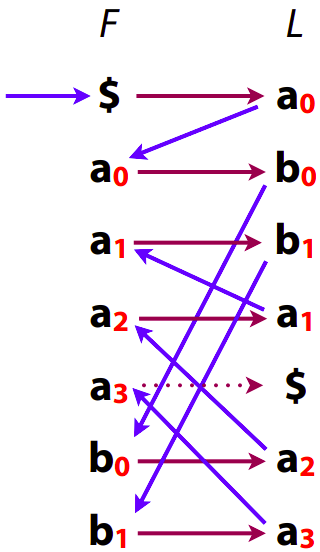
\includegraphics[width=80px]{./img/BWT_3.png}
		\caption{Burrows-Wheeler transformace zpětné získání původního řetězce. \cite{bw_transform}}
		\label{fig:bw_transform_inverse}
\end{figure}

\noindent
Díky vztahu mezi F a L sloupcem je možné vyhledávat daný řetezec (zobrazeno na obrázku \ref{fig:fm_index}). Například vyhledáváný řetězec bude $P = aba$. Při pohledu do F sloupce jsou nalezeny všechy sloupce začínající $a$, následně v L sloupci ve stejných řádcích jsou nalezeny dva výskyty $b$. Již je získán sufix $ba$, který existuje. Pokračuje se dále na řádky, které začínají právě nalezenými $b$. V sloupci L pro dané řádky je nalezena $a$. Řětezec $P = aba$ se v textu vyskytuje. 

\begin{figure}[H]
		\centering
		\begin{subfigure}[t]{.4\textwidth}
			\centering
			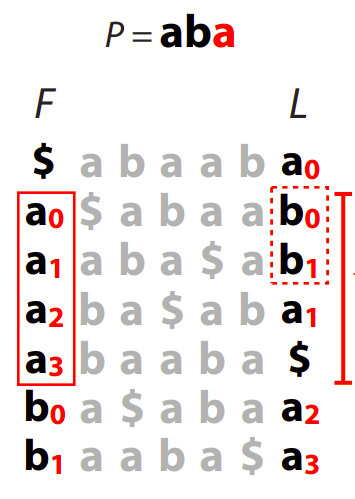
\includegraphics[width=100px]{./img/FM_index_1.png}
		\end{subfigure}
		%
		\begin{subfigure}[t]{.4\textwidth}
			\centering
			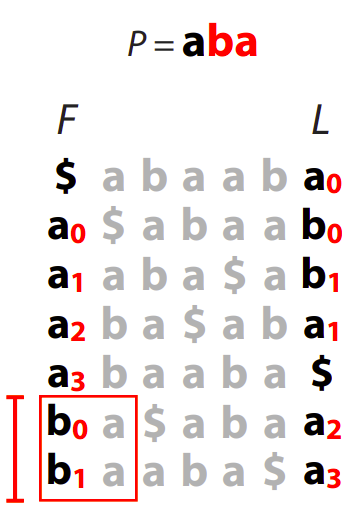
\includegraphics[width=100px]{./img/FM_index_2.png}
		\end{subfigure}	
		\caption{FM index - získání prefixu. \cite{bw_transform}}
		\label{fig:fm_index}
\end{figure}


\section{Další pomocné metody}
\subsection{Levenshteinova vzdálenost}
Levenshteinova vzdálenost zjišťuje rozdílnost dvou textů na základě počtu změn, které je třeba udělat, aby byl z jednoho řetězce získán druhý řetezec. Za úpravy se považuje vložení, smazání a nahrazení. Algortimus funguje tak, že se snaží ze slova, které bylo předáno jako první v argumentu vytvořit slovo předáné jako druhý argument. Příkladem může být vzdálenost mezi řetězci \textit{SPAM} a \textit{PARK}.  Vzdálenost těchto slov je 3. Výstup v případě python knihovny je možné vidět následovně. Výstup \ref{leve_1} je v případě SPAM, PARK. Výstup \ref{leve_2} je v případě PARK, SPAM. Změny jsou definovány: o jakou změnu jde, index znaku v prvním řetězci a index znaku v druhém řetězci. Je možné si všimnout závislosti mezi těmito dvěma postupy. \cite{levenshrein_baku}


\begin{align}
   \label{leve_1} ('delete', 0, 0), ('insert', 3, 2), ('replace', 3, 3) \\
    SPAM -> \_PAM -> \_PARM -> PARK \nonumber
\end{align}

\begin{align}
   \label{leve_2} ('insert', 0, 0), ('delete', 2, 3), ('replace', 3, 3) \\
    PARK -> SPARK -> SPAR\_ -> SPAM \nonumber
\end{align}



\chapter{Implementace}
\section{Popis problému}
Hlavním úkolem navrhnutého nástroje je určit alely, které představují ready ze sekvenátoru. Jednou z výzev je, že alela může být dlouhá až téměř 16 000 bp. Získané ready jsou ale dlouhé jen 250 bp a navíc mohou obsahovat chyby (záměna bází, chybějící báze nebo báze navíc). 

\section{Referenční geny}
Referenční geny byly převzaty z IPD-KIR \cite{imgt_hla_database}, konkrétně soubory ve formátu \textit{fasta} uloženy ve stejnojmené složce. Jednotlivé soubory jsou pojmenovány genem, který obsahují, např. \textit{KIR2DL1\_gen.fasta}. Každý soubor představuje všechny dostupné alely konkrétního genu. Jedinou výjimku tvoří soubory \textit{KIR\_gen.fasta} či \textit{KIR\_nuc.fasta}, které obsahují všechny geny, a navíc i pseudogeny. 
\\
\\
Kromě souborů \textit{*\_gen.fasta} obsahuje složka \textit{fasta} také soubory \textit{*\_prot.fast} a \textit{*\_nuc.fasta}. Soubor \textit{\_gen.fasta} obsahuje informace o celých genech. Oproti tomu \textit{\_nuc.fasta} obsahuje nukleotidy, tedy pouze exony bez intronů. Soubor \textit{*\_prot.fast} obsahuje sekvence proteinů, které vznikly z RNA. Data získaná z nemocnice budou odpovídat alelám uvedených v \textit{\_gen.fasta}. V práci bude jako reference použit soubor $\_gen$.
\\
\\
Při analýze porovnávání souboru \textit{nuc} a \textit{gen} bylo zjištěno, že v souboru \textit{nuc} je více alel než v souboru \textit{gen}. Konkrétně v souboru \textit{gen} je 461 alel a v souboru \textit{nuc} je 1109 alel. Tento údaj  mimo jiné dokazuje, že nejsou přístupné referenční sekvence ke všem reálným alelám. Nejmenší Levenshteinova vzdálenost mezi alelami je 1, největší 15 943 a průměrná 4768.98. 
\\
\\
Na následujícím obrázku je možné vidět všechny vzdálenosti ostatních alel ve skupinkách podle genů vzhledem k alele 3DS1*0130101. Je možné si povšimnout, že nejblíže má k alelám ze stejného genu.

\begin{figure}[H]
    \centering
    \def\svgwidth{\columnwidth}
    \import{svg/}{KIR3DS1cross_gens.pdf_tex} 
\end{figure}

\noindent
Následující obrázek zobrazuje vzdálenosti pouze v rámci genu 3DS1 opět k alele 3DS1*0130101.
\begin{figure}[H]
	\centering
    \def\svgwidth{300px}
    \import{svg/}{exp1_KIR3DS1_distance.pdf_tex} 
\end{figure}

\section{Testovací KIR genomy}
Genomy, na kterých byl nástroj testován, byly dodány vedoucí práce a vychází ze známých genotypů KIR - Genotype Reference List uvedených v \cite{kir_genotypes_10}. Genomy test1 - test11 byly sestaveny podle definovaných genotypů a umýslně vybrány, ty které představují určitým způsobem výzvu pro navrhnutý nástroj. Přesný obsah testovacích genomů je uveden v příloze.



\section{Návrh systému}
Systém byl navržen jako modulární, díky čemuž je možná jednoduchá náhrada jakékoliv jeho části. 
\\
\\ 
Vše začíná získáním readů, pro něž má být vyhodnoceno, jaké KIR alely představují. První možností je použít data přímo z FN Plzeň/BC LF UK Plzeň. Tyto data představují ready, na kterých bude prováděna verifikace nástroje. Druhou možností je ready simulovat. Na těchto datech byl nástroj vyvíjen a laděn. Genom může být vyroben manuálně nebo ho lze vyrobit za pomoci skriptu. V dalším kroku musí být vytvořený genom "rozbit" \space do podoby, jako by vyšel ze sekvenátoru. Rozdělí se na ready a vytvoří se v něm chyby, aby data co nejvíce odpovídala reálným. To se provádí za pomoci nástroje ART.
\\
\\
V následující části jsou získaná data, tedy ready, zarovnána na referenční genom pomocí nástroje Bowtie2. Nakonec je zarovnání vyhodnoceno a rozpoznáno, o jaké alely genů se pravděpodobně jedná. Vyhodnocení je rozděleno do několika experimentů.

\begin{figure}[H]
		\centering
		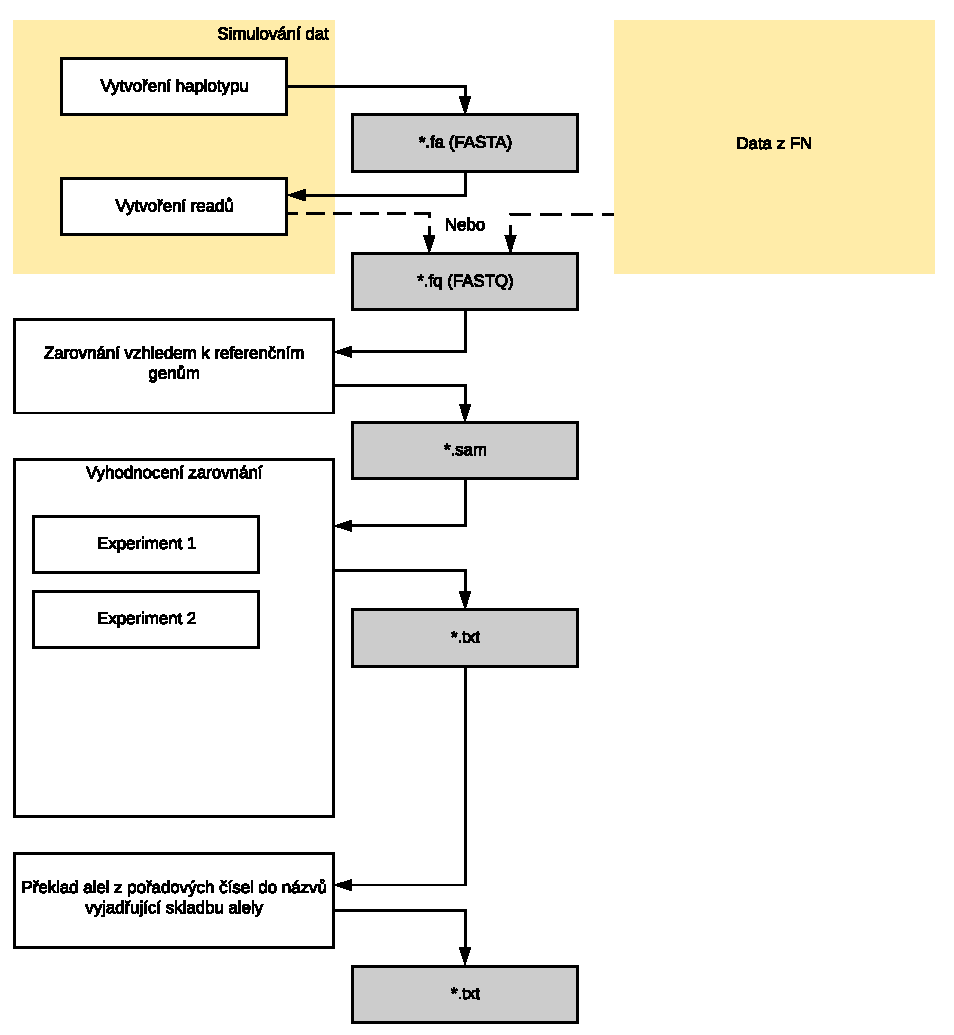
\includegraphics[width=\textwidth]{./img/navrh_systemu.pdf}
		\caption{Návrh systému. }
		\label{fig:navrh_systemu}
\end{figure}

\subsection{Použité programové prostředky}
Program byl navržen a implementován na operačním systému Linux za použití programovacího jazyka Python. Tento jazyk byl zvolen z důvodu jednoduchého použití, díky čemuž nebyl vývoj prototypů časově náročný. Pro spuštění programu je nutné mít nainstalovaný Python ve verzi 3.8, nástroj ART ve verzi MountRainier, Bowtie 2 ve verzi 2.4.1. Dále byly použity Python knihovny pysam ve verzi 0.14, python-Levenshtein, Matplotlib a Numpy.
\\
\\
Pysam je modul do Pythonu, který pomáhá číst a manipulovat s výstupními soubory ze zarovnávačů.
Python-Levenshtein je modul do pythonu který obsahuje funkce na výpočet Levenhsteinovy vzdálenosti a zaroveň dokáže vrátit pozice rozdílných znaků v řetězci.
Matplotlib je rozsáhlá knihovna pro vytváření animací a interaktivních vizualizací v Pythonu. V práci byla použita pro vykreslování grafů.

\section{Modulové jednotky programu}
Vše potřebné pro samotný běh programu obstarává skript $run.py$ spolu s nastavením v souboru $config.py$. Skript $run.py$ postupně pouští jednotlivé moduly. Díky nastavení v $config.py$ je možné si zvolit spuštění jen některých modulů. Například pouhé vytvoření testovacích dat nebo pouze jejich zarovnání, a v neposlední řádě spouštění vyhodnocování zarovnávaných dat.

\subsection{Config}
S konfiguračním souborem \textit{config.py} jsou spojeny všechny skripty a obsahuje jejich veškerá nastavení. Jak již bylo zmíněno, je možné pomocí tohoto nastavení spustit jednotlivé moduly. Jedná se především o položky \textit{CREATE\_READS}, \textit{ALIGN} a \textit{IDENTIFY}. \textit{CREATE\_READS} udržuje informaci o spuštění vytvoření syntetických readů. \textit{ALIGN} se stará o spuštění zarovnání. V neposlední řadě \textit{IDENTIFY}, která řídí spuštění vyhodnocení zarovnání. V případě nastavené hodnoty \textit{IDENTIFY} na \textit{True} je možné řídit spouštění experimentů (položky \textit{EXP1}, \textit{EXP2} a \textit{EXP3}). Důležitou položkou v configu jsou cesty ke zdrojovým a výstupním složkám. Dalším nastavením je obsah genomů při případném vygenerování testovacích dat.


\subsection{Simulování dat}
O simulování dat se stará skript \textit{create\_syntetic\_reads.py}, přičemž toto simulování je rozděleno na dva kroky: vytvoření genomů a vytvoření readů. Mezi těmito dvěma fázemi vznikají soubory s příponou \textit{.fa}. Každý tento soubor obsahuje právě jeden KIR genom. Tyto genomy jsou následně použity jako vstupní soubor pro vytvoření readů, které se provádí za pomocí nástroje ART. Pro vytvoření genomů je volán skript \textit{create\_genome.py}, který vytvoří genomy na základě nastavení v configu pod položkou \textit{GENOMES} a za pomoci referenčních genů v souboru pod položkou v configu \textit{REFERENCE\_KIR\_GENS\_FILE}. Vytvoření probíhá obdobně jako je popsáno níže u manuálního vytvoření testovacího genomu. Výsledné genomy jsou uloženy do adresáře z configu \textit{GENOME\_FOLDER}. Výstupem modulu \textit{create\_syntetic\_reads} je soubor s příponou \textit{.fq}, který by měl odpovídát formátu reálných dat, které byly dodány. Výstupní soubory jsou uloženy do složky pod proměnnou \textit{READS\_FOLDER}.
\\
\\
\textbf{Manuální vytvoření testovacího genomu} lze provést následujícím způsobem. V prvním kroku je v referenčním souboru vybrána konkrétní alela genu. Někdy je možné najít takovou shodu, kdy se alely liší jen v konečné části jejich označení a v genomu je pouze prvních 5 čísel. V tomto případě může být vložena jakákoli z těchto alel. Vkládaná alela musí být vložena včetně její hlavičky tedy: \textit{>KIR:KIR00138 \: KIR3DL3*0040201 \: 12390 \: bp}.

\subsection{Zarovnání vzhledem k referenčním genům}
Zarovnávání obstarává skript \textit{alignment\_reads\_to\_reference.py} s pomocí nástroje Bowtie2. V souboru \textit{config.py} je nutné vyplnit položku \textit{BOWTIE\_} \\ \textit{HOME\_DIRECTORY} podle umístění nástroje Bowtie na konkrétním počítači. V prvním kroku jsou vytvořeny Bowtie2 indexy, které je možné použít napříč běhy, proto je v nastavení položka \textit{BOWTIE\_BUIL\_INDEX}, díky které je možné toto vytvoření povolit nebo zakázat. Bez vytvořených indexů, tedy indexů z minulých běhů, ale Bowtie2 nebude zarovnávat. Bowtie2 vytváří indexy na základě obsahu souboru \textit{REFERENCE\_KIR\_GENS\_FILE}. V dalším kroku jsou načteny všechny ready ze složky v \textit{READS\_FOLDER} a nasledně jsou zarovnány nástrojem Bowtie2. Tady je nutné, aby byly ready paired-end, tedy aby se vyskytovaly dvakrát, příčemž jednou s \textit{1} na konci a podruhé s \textit{2}. Tento předpoklad zajistí správné nastavení ARTU, který je takto nastaven. Výstupní soubory jsou ve formátu \textit{.sam} a jsou umístěny dle položky \textit{ALIGMENT\_FOLDER} v nastavení. 

\subsection{Přístupy k identifikaci alel}
Detailní výsledky pro všechny genomy je možné najít v příloze. V následující teoretické části jsou uvedeny vždy simulované genomy.

\subsubsection{Experiment 1}
Jako první pokus o určení alel, které by mohly být obsaženy v genomu, bylo pouhé oříznutí alel, které by měly větší procentuální šířku zarovnání (například 90 \%).  V případě buněčné linie AMALA, která byla simulována nástrojem ART a která obsahuje 19 alel, je výsledek zobrazen níže. Červeně jsou označený alely, které se v genomu skutečně nacházejí a číslo v závorce udává jejich procentuální pokrytí. Pravděpodobným důvodem proč mají alely, které do genomu nepatří tak vysoké zarovnání, je jejich podobnost. Například alely 2DS4*0010101 a 2DS4*0010102 jejiž vzdálenost je 2. Z toho lze logicky usoudit, že na alelu 2DS4*0010102 se zarovnaly některé z readů alely 2DS4*0010101.

\begin{multicols}{2}
\begin{itemize}
	\itemsep0em
	\item \textcolor{red}{3DL2*0070102 (99.64\%) }
	\item \textcolor{red}{2DS4*0010101 (99.64\%) }
	\item 2DS4*0010102 (99.55\%)
	\item \textcolor{red}{2DS5*0020101 (99.50\%) }
	\item \textcolor{red}{3DL2*0020105 (99.48\%) }
	\item \textcolor{red}{2DS2*0010101 (99.43\%) }
	\item \textcolor{red}{3DL3*00802 (99.34\%) }
	\item 3DL2*0070103 (99.29\%) 
	\item \textcolor{red}{3DL3*0040201 (99.22\%) }
	\item 3DL2*0020106 (99.15\%)
	\item \textcolor{red}{3DP1*007 (99.04\%) }
	\item 2DS4*0010107 (98.99\%)
	\item 2DS5*0020103 (98.98\%)
	\item 3DS1*055 (98.70\%)
	\item 3DL2*0020102 (98.40\%)
	\item 3DL2*0020104 (98.19\%)
	\item 3DL2*018 (98.07\%)
	\item 2DL2*0030101 (98.07\%)
	\item 2DP1*0020105 (97.99\%)
\end{itemize}
\end{multicols}

\noindent
Následně jsou uvedeny alely, které do genomu patří, mají pokrytí více než 90 \%, ale nejsou v prvních 19.
\begin{multicols}{2}
\begin{itemize}
	\itemsep0em
	\item 2DL2*0030102 (97.29\%)
	\item 2DL3*0010109 (94.16\%)
	\item 2DL5A*00102 (96.6\%)
	\item 2DS1*0020106 (96.57\%)
	\item 3DP1*0090101 (96.46\%)
	\item 3DS1*130101 (95.83\%)
\end{itemize}
\end{multicols}


\noindent
Nakonec jsou uvedené alely, které do genomu patří, ale mají pokrytí menší než 90 \%. Po tomto zjištění se nabízí pokusit se snížit požadované zarovnání na 70 \% a přidat další upřesnující kroky.

\begin{multicols}{2}
\begin{itemize}
	\itemsep0em
	\item 2DL1*0030201 (81.8\%)
	\item 3DL1*0150201 (70.71\%)
\end{itemize}
\end{multicols}

\noindent
Ná následujícím obrázku jsou zobrazeny všechny alely genu KIR3DS1 a jeich zarovnání. Červeně je označena alela, která do genomu AMALA patří. Je možné si povšimnout, že alela s největším pokrytím do genomu nepatří. Navíc pokrytí větší než 90 \% mají všechny alely až na jednu. Neméně důležité je, že poslední alela má značně kratší délku než všechny ostatní alely stejného genu. Poslední věcí je hloubka pokrytí, která by díky nastavení sekvenátoru měla odpovídat hladině 100 u alely, která do genu patří. Jak je vidět z obrázku, hloubka pokrytí se u většiny alel pohybuje v extrémech kolem 20. Z toho lze odvodit, že ready alely 3DS1*0130101 byly pravděpodobně rozděleny mezi všechny alely tohoto genu.

\begin{figure}[H]
    \centering
    \def\svgwidth{\columnwidth}
    \import{svg/}{exp1_KIR3DS1.pdf_tex} 
\end{figure}

\noindent
Všechny výše uvedené analýzy vybízí k bližšímu prozkoumání podobnosti alel. Níže jsou uvedeny grafy Levenshteinovy vzdálenosti ostatních alel stejného genu vzhledem k alele 3DS1*0130101, tedy té, která je obsažena v genomu.

\begin{figure}[H]
	\centering
    \def\svgwidth{\columnwidth}
    \import{svg/}{exp1_KIR3DS1_distance.pdf_tex} 
\end{figure}

\begin{figure}[H]
	\centering
    \def\svgwidth{\columnwidth}
    \import{svg/}{exp1_KIR3DS1_distance_100.pdf_tex} 
\end{figure}
 
\noindent
Z předchozích obrázků je patrné, že 3 alely jsou vzdálené v rámci jednotek, 9 alel je vzdálených kolem 500 a jen jedna alela je vzdálená více, což pravděpodobně způsobuje to, že je kratší. Přichází tedy na řadu otázka, jak určit, které alely jsou si až moc podobné, a pak rozhodnout, kterou z nich odstranit. Vzdálenost, kdy jsou si alely blízké je možné nastavit v configu pod položkou \textit{CLOSE\_DISTANCE}. Dále je porovnáváno jejich pokrytí v místech, kde jsou rozdílné. Pokud je hloubka pokrytí jedné alely 2krát větší než hloubka pokrytí druhé alely, je druhá alela odstřižena.
\\
\\
V tabulce níže je uvedeno porovnání výsledků požadovaného pokrytí 90 \% a 70 \% u genomu AMALA. Za blízké byly alely považovány v případě vzdálenosti menší než 100. Genom AMALA obsahuje celkem 19 alel a žádná z nich se neopakuje. Krok 1 je pouze statistika prvního zarovnání. Obsahuje všechny alely, které jsou v referenci. Celkově je v referenci 461 alel. Pouze dva geny ze všech genů uvedených v referenčmí sekvenci se nenacházejí v tomto genomu. Krok 2 je po odstřižení alel, které mají pokrytí menší než 90 \%, případně 70 \%. V posledním kroku 3 jsou uvedené výsledky po odstřižení podobných. 
\\
\\
\begin{center}
\tiny
\rowcolors{2}{gray!25}{white}
\begin{tabular}{c || c || c | c l | c l || c | c l | c l }
& Krok 1 & \multicolumn{5}{c||}{Krok 2} & \multicolumn{5}{c}{Krok 3} \\ 
& \Gape[0pt][2pt]{\makecell[c]{Zbývá \\ alel}} & \Gape[0pt][2pt]{\makecell[c]{Zbývá \\ alel}} & \multicolumn{2}{c|}{Ztraceno} & \multicolumn{2}{|c||}{\Gape[0pt][2pt]{\makecell[c]{Geny \\ navíc}}} & \Gape[0pt][2pt]{\makecell[c]{Zbývá \\ alel}} & \multicolumn{2}{c}{Ztraceno} & \multicolumn{2}{|c}{\Gape[0pt][2pt]{\makecell[c]{Geny \\ navíc}}}  \\
\hline
\hline
\Gape[0pt][2pt]{\makecell[c]{amala \\ pokrytí \\ 90 \%}} & 461 & 113 & 2 & \Gape[0pt][2pt]{\makecell[l]{2DL1*0030201 \\ 3DL1*0150201}} & 0 &  -  & 23 & 4 & \Gape[0pt][2pt]{\makecell[l]{3DP1*0090101 \\ 2DL4*0010201}} & 0 &  -  \\ 

\Gape[0pt][2pt]{\makecell[c]{amala \\ pokrytí \\ 70 \%}} \% & 461 & 193 & 0 &  -  & 0 &  -  & 41 & 2 & \Gape[0pt][2pt]{\makecell[l]{2DL4*0010201 \\ 3DP1*0090101}} & 0 &  -  \\ 
\end{tabular}
\captionof{table}{Výsledky experimentu 1 u genomu AMALA. Odřezány byly alely, které měly pokrytí menší než 90 \%. \textit{Alel} u genomu značí počet v daném genomu. Číslo v závorkách udává, kolik alel je v daném genomu dvakrát. V každém kroku \textit{zbývá alel} je kolik alel ještě zůstalo ve výběru, \textit{ztraceno} určuje kolik alel má být v genomu, ale algoritmus je vyřadil. Za tímto číslem jsou vypsané alely, které byly ztraceny. V dalších krocích jsou vypsány alely bez těch, které už byly ztraceny v předchozích krocích. Obdobně je to s \textit{geny navíc}, které udávají počet a druh genů již neobsahujích žádnou z alel, která náleží do daného genomu. }
\end{center}

\noindent
Ve výsledků v příloze jistě zaujme genom Test7, který ztratil 7 alel v rámci třetího kroku. Tedy při odřezávání podobných alel.

\newpage
\begin{center}
\tiny
\rowcolors{2}{gray!25}{white}
\begin{tabular}{ c | c l | c l || c | c l | c l || c | c l | c l }
\multicolumn{5}{c||}{Krok 1} & \multicolumn{5}{c||}{Krok 2} & \multicolumn{5}{c}{Krok 3} \\ 
\Gape[0pt][2pt]{\makecell[c]{Zbývá \\ alel}} & \multicolumn{2}{c}{Ztraceno} & \multicolumn{2}{|c||}{\Gape[0pt][2pt]{\makecell[c]{Geny \\ navíc}}} & \Gape[0pt][2pt]{\makecell[c]{Zbývá \\ alel}} & \multicolumn{2}{c|}{Ztraceno} & \multicolumn{2}{|c||}{\Gape[0pt][2pt]{\makecell[c]{Geny \\ navíc}}} & \Gape[0pt][2pt]{\makecell[c]{Zbývá \\ alel}} & \multicolumn{2}{c}{Ztraceno} & \multicolumn{2}{|c}{\Gape[0pt][2pt]{\makecell[c]{Geny \\ navíc}}}  \\
\hline
\hline
461 & 0 &  -  & 8 & \Gape[0pt][2pt]{\makecell[l]{2DS1 \\ 3DS1 \\ 2DL2 \\ 2DL5B \\ 2DS2 \\ 2DS3 \\ 2DL5A \\ 2DS5}} & 188 & 0 &  -  & 0 &  -  & 24 & 7 & \Gape[0pt][2pt]{\makecell[l]{2DL4*0010201 \\ 3DL1*0150203 \\ 2DL3*0010103 \\ 2DP1*0020106 \\ 2DS4*0010107 \\ 3DL3*0090103 \\ 2DL1*0030205}} & 0 &  -
\end{tabular}
\captionof{table}{Výsledky experimentu 1 u genomu Test7. Odřezány byly alely, které měly pokrytí menší než 70 \%. \textit{Alel} u genomu značí počet v daném genomu. Číslo v závorkách udává kolik alel je v daném genomu dvakrát. V každém kroku \textit{zbývá alel} je kolik alel ještě zůstalo ve výběru, \textit{ztraceno} určuje kolik alel má být v genomu, ale algoritmus je vyřadil. Za tímto číslem jsou vypsané alely, které byly ztraceny. V dalších krocích jsou vypsány alely bez těch, které už byly ztraceny v předchozích krocích. Obdobně je to s \textit{geny navíc}, které udávají počet a druh genů již neobsahující žádnou z alel, která náleží do daného genomu.  }
\end{center}

\noindent
Jednou ze smazaných alel je i 2DL4*0010201, která byla smazána kvůli alele KIR2DL4*0010305, taktéž patřící do genomu. Vzdálenost mezi těmito alelami je 10. Suma hloubky pokrytí alely KIR2DL4*0010201 v místě kde se alely neshodují je 63. U alely KIR2DL4*0010305 je to 154. 


\begin{figure}[H]
	\centering
    \def\svgwidth{\columnwidth}
    \import{svg/}{exp1_2DL4_0010201.pdf_tex} 
\end{figure}

\begin{figure}[H]
	\centering
    \def\svgwidth{\columnwidth}
    \import{svg/}{exp1_2DL4_0010305.pdf_tex} 
\end{figure}

\noindent
Po analyzování všech smazaných alel se ukázalo, že všechny byly smazány kvůli alele, která do genomu také patří.

\subsubsection{Experiment 2}
Experiment 2 byl navržen tak, aby zarovnávání probíhalo ve více iterací. Mělo by pak být v dalších krocích jasnější, která alela do genomu skutečně patří a která ne, díky tomu, že ready zarovnané na odstřižené alely by se měly zarovnat na alely, které zbývají, a tak podpořit alely patřící do genomu. 
\\
\\
V první fázi se provede zarovnání na celou KIR referenci. V kroku 1 je vytvořena statistika obdobně jako v prvním experimentu a jsou odstřiženy alely, které mají menší pokrytí než $CUT\_COVERAGE\_ALELS$, které je uvedené v $configu$. Ze zbylých alel je vytvořená nová reference, na kterou je provedeno nové zarovnání readů. Opět je vytvořena statistika. Výsledky této statistiky nalezneme v kroku 2. Následuje krok 3, v němž soutěží podobné alely v rámci jednoho genu. Podobnost alel je určována na základě Levenshteinovy vzdálenosti. Alely jsou si podobné v případě, kdy je jejich vzdálenost menši než vzdálenost uvedená v $configu$ pod parametrem $CLOSE\_DISTANCE$. Následuje vytvoření nové reference a nové zarovnání.  


\noindent
Na následujících obrázcích je vidět alela 2DL1*0030201 genomu AMALA. První obrázek značí její zarovnání po prvním kroku. Druhý obrázek ukazuje její zarovnání po druhém kroku. V tomto případě bylo zarovnání jednoznačně ku prospěchu.

\begin{figure}[H]
	\centering
    \def\svgwidth{\columnwidth}
    \import{svg/}{exp2_step1_2DL1.pdf_tex} 
\end{figure}

\begin{figure}[H]
	\centering
    \def\svgwidth{\columnwidth}
    \import{svg/}{exp2_step2_2DL1.pdf_tex} 
\end{figure}

\noindent
Ovšem je možné se potkat i s alelami, kde pokrytí zarovnání klesne, jako v případě 2DL3*0010109 genomu AMALA.

\begin{figure}[H]
	\centering
    \def\svgwidth{\columnwidth}
    \import{svg/}{exp2_step1_2DL3.pdf_tex} 
\end{figure}

\begin{figure}[H]
	\centering
    \def\svgwidth{\columnwidth}
    \import{svg/}{exp2_step2_2DL3.pdf_tex} 
\end{figure}

\noindent
Následující tabulka zobrazuje základní porovnání mezi výsledky experimentu 1 a experimentu 2. Je patrné, že genomu AMALA více zarovnání prospělo. Bylo vyřazeno více alel, které do genomu nepatří. Naopak u genomu RSH došlo ke zhoršení výsledků.


\begin{center}
\tiny
\rowcolors{2}{gray!25}{white}
\begin{tabular}{ c  c || c | c l | c l || c | c l | c l }
& & \multicolumn{5}{c||}{Krok 2} & \multicolumn{5}{c}{Krok 3} \\ 
genom & & \Gape[0pt][2pt]{\makecell[c]{Zbývá \\ alel}} & \multicolumn{2}{c|}{Ztraceno} & \multicolumn{2}{|c||}{\Gape[0pt][2pt]{\makecell[c]{Geny \\ navíc}}} & \Gape[0pt][2pt]{\makecell[c]{Zbývá \\ alel}} & \multicolumn{2}{c}{Ztraceno} & \multicolumn{2}{|c}{\Gape[0pt][2pt]{\makecell[c]{Geny \\ navíc}}}  \\
\hline
\hline
amala exp 1 & 19 (0) & 193 & 0 &  -  & 0 &  -  & 41 & 2 & \Gape[0pt][2pt]{\makecell[l]{2DL4*0010201 \\ 3DP1*0090101}} & 0 &  - \\ 
amala exp 2& 19 (0) & 193 & 0 &  -  & 0 &  -  & 38 & 2 & \Gape[0pt][2pt]{\makecell[l]{2DL4*0010201 \\ 3DP1*0090101}} & 0 &  -  \\
\hline 
rsh exp 1 & 20 (0) & 228 & 0 &  -  & 1 &  2DL5A & 40 & 2 & \Gape[0pt][2pt]{\makecell[l]{2DP1*0020110 \\ 2DL1*0030205}} & 1 &  -  \\ 
rsh exp 2 & 20 (0) & 228 & 0 &  -  & 1 & 2DL5A & 44 & 2 & \Gape[0pt][2pt]{\makecell[l]{2DP1*0020110 \\ 2DL1*0030205}} & 1 &  -   \\ 

\end{tabular}
\captionof{table}{Porovnání experimentu 1 a experimentu 2 při stejném nastavení. Odřezány byly alely, které měly pokrytí menší než 70 \%. Za podobné byly alely považovány v případě, kdy byla jejich vzdálenost nižší než 100. \textit{Alel} u genomu značí počet v daném genomu. Číslo v závorkách udává kolik alel se v daném genomu vyskytuje dvakrát.  V každém kroku \textit{zbývá alel} je kolik alel ještě zůstalo ve výběru, \textit{ztraceno} určuje kolik alel má být v genomu, ale algoritmus je vyřadil. Za tímto číslem jsou vypsané alely, které byly ztraceny. V dalších krocích jsou vypsány alely bez těch, které už byly ztraceny v předchozích krocích. Obdobně je to s \textit{geny navíc}, které udávají počet a druh genů již neobsahující žádnou z alel, která náleží do daného genomu.  }
\end{center}


\noindent
Na následujícím obrázku je výsledek genomu AMALA genu 2DL2 po třetím kroku. Alela, která do genomu patří, má jasný vrchol. Tento vrchol označuje místo, kde bylo zarovnáno mnoho readů. 

\begin{figure}[H]
	\centering
    \def\svgwidth{\columnwidth}
    \import{svg/}{exp2_2DL2_peak.pdf_tex} 
\end{figure}

\noindent 
Oproti tomu u genu 3DS1 po kroku 3 jsou zbývající alely k nerozeznání. 

\begin{figure}[H]
	\centering
    \def\svgwidth{\columnwidth}
    \import{svg/}{exp2_3DS1_peak_problem.pdf_tex} 
\end{figure}

\noindent
Výsledkem kroku 4 je odstranění alel v případě, kdy sdílejí gen s alelami s jednoznačným vrcholem, ale u genů, kde to neni jasné, nic odstraňovat nebudou. Pro každý gen je spočítána hloubka pokrytí pro jednu alelu. Z jednoho genu jsou porovnávány každá alela s každou. Pokud alela1 má 2krát větší maximální hloubku pokrytí než alela2 a zároveň je maximální histogram alely1 2krát větší než průměrná hloubka pokrytí pro všechny alely daného genu, je alela2 odstraněna.
\\
\\
V následující tabulce je porovnání genomu AMALA a kroku 3 a 4. Díky kroku 4 byl algortimus zpřesněn a odstraněno 19 alel, které do genomu nepatří za cenu ztracení jedné alely, která do genomu patří. Jelikož v praxi je mnohem lepší alelu ztratit než určit že se v genomu nachází alela, která tam skutečně není, dá se říci, že u tohoto genomu byl krok 4 prospěšný, stejně jako u ostatních genomů.

\begin{center}
\tiny
\rowcolors{2}{gray!25}{white}
\begin{longtable}{l c|| c | c l | c l || c | c l | c l }
 & & \multicolumn{5}{c||}{Krok 3} & \multicolumn{5}{c}{Krok 4}  \\ 
Genom & Alel & \Gape[0pt][2pt]{\makecell[c]{Zbývá \\ alel}} & \multicolumn{2}{c|}{Ztraceno} & \multicolumn{2}{|c||}{\Gape[0pt][2pt]{\makecell[c]{Geny \\ navíc}}} & \Gape[0pt][2pt]{\makecell[c]{Zbývá \\ alel}} & \multicolumn{2}{c}{Ztraceno} & \multicolumn{2}{|c}{\Gape[0pt][2pt]{\makecell[c]{Geny \\ navíc}}} \\
\hline
\hline
amala & 19 (0) &  38 & 2 & \Gape[0pt][2pt]{\makecell[l]{2DL4*0010201 \\ 3DP1*0090101}} & 0 &  -  & 18 & 3 & 3DL2*0020105 & 0 &  - \\ 
\end{longtable}
\end{center}

\begin{figure}[H]
		\centering
		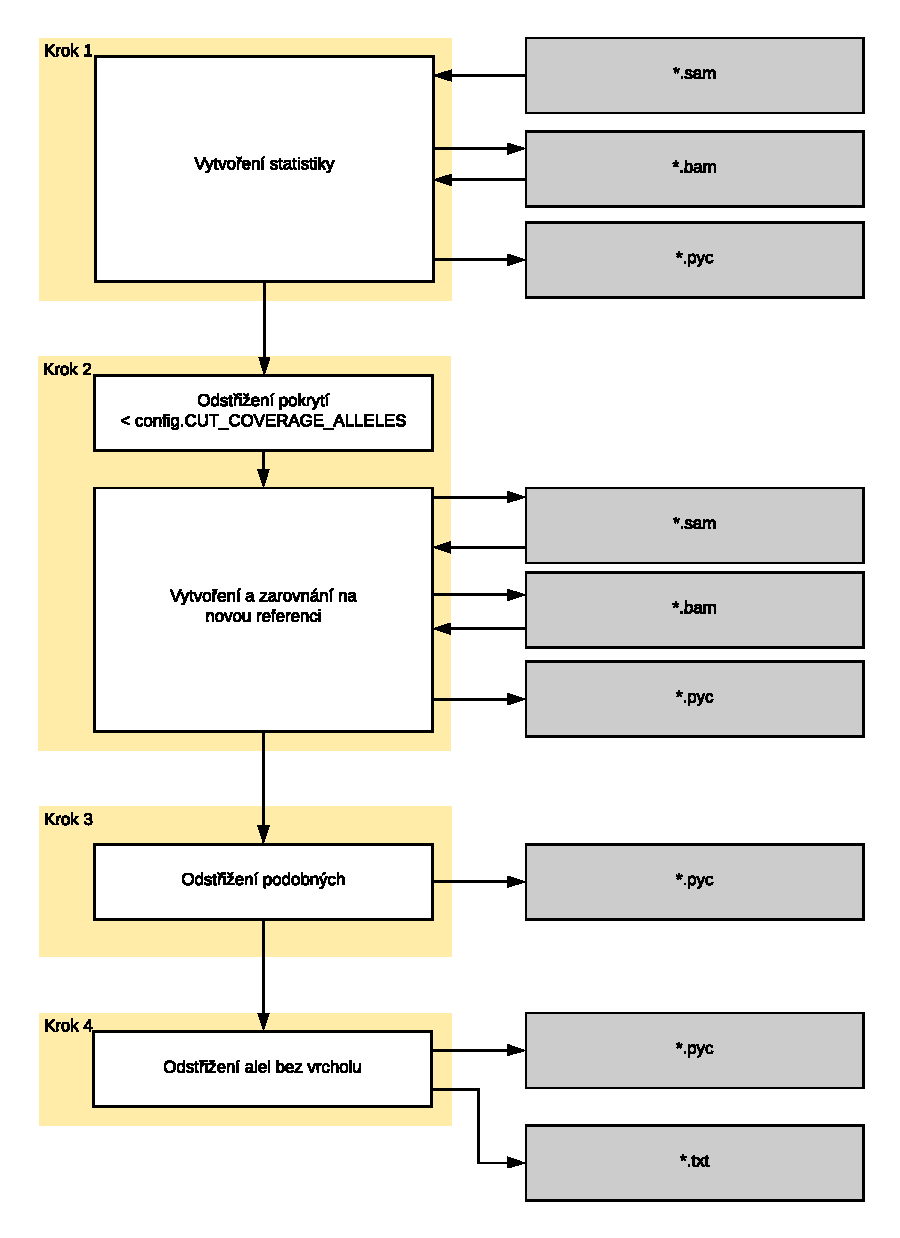
\includegraphics[width=\textwidth]{./img/exp2_diagram.pdf}
		\caption{Postup algoritmu experimentu 2. }
		\label{fig:exp2_diagram}
\end{figure}

\subsubsection{Experiment 3}
Další experiment byl založen na omezení stavového prostoru vytvořením clusterů. Alely jsou seřazeny od nejvíce pokryté po nejméně pokrytou. První alela s největším pokrytím je vložená do prvního clusteru. Další alely projdou všechny clustery a pokud je vzdálenost alespoň jedné alely z clusteru a právě procházející alely menší než $CLUSTER\_DISTANCE$ uvedená v $configu$, je alela přiřazena do tohoto clusteru. Pokud ne, pokračuje v porovnávání dokud nezkontroluje všechny clustery. V případě, kde nezapadá ani do jednoho z clusterů, vytvoří nový. Následně jsou porovnány všechny alely z clusteru. Pokud alespoň jedna alela v daném clusteru má pokrytí větší než $CUT\_COVERAGE\_ALLELES$ uvedené v $configu$, není žádná alela v daném clusteru smazána. V opačném případě jsou všechny alely z clusteru smazány. Další postup je stejný s experimentem 2. 
\\
\\
Výhodou tohoto přístupu by mělo být zamezení smazání alel, které do genomu patří, ale jejichž ready se zarovnaly na alelu jí podobnou. 
\\
\\
Při vzdálenosti 5 bylo vytvořeno kolem 224 clusterů, přičemž jich může být o pár jednotek více nebo méně z toho důvodu, že alely nejdou za sebou ve stejném pořadí, ale v pořadí od nejvíce pokrytých po nejméně pokryté. Při vzdálenosti 10 vznikalo kolem 171 clusterů, při vzdálenosti 15 vznikalo 143, a nakonec při vzdálenosti 30 vznikalo kolem 122 clusterů. Takto navržené clusterování nepřineslo očekávaná zlepšení. Je třeba se nad clustrováním alel zamyslet jinak. Na příkladech clusterů uvedených v příloze si lze povšimnout, že většinou alely pocházely ze stejných genů.


\subsubsection{Návrh na experiment 4}
Clustery se vytváří zejména z toho důvodu, že si alely mezi sebou \space "kradou" ready. Možným vylepšením clusterů by mohlo být dát dohromady ty alely, které mají minimální rozdíl v 250 dlouhém useku oproti jiné (protože ready jsou dlouhé 250bp). Následně si pak mohlo vyhledat kolik takových úseků má jedna alela společných s jinou. Problémem tohoto návrhu bude výpočetní náročnost.
 
\subsubsection{Zhodnocení experimentů}
Mezi problematické geny lze řadit 2DL5B a 2DL5A, které často měly vysoké pokrytí bez toho aby jakákoliv z jejich alel byla v genomu. Častou ztratovost vykazoval gen 3DL1. Pro zajímavost v případě genomu Test1 bylo po prvním kroku experimentu 2 maximální pokrytí jeho alel 72 \%. V kroku následujcím toto číslo poskočilo na 93 \%. 


\chapter{Porovnání přístupů k identifikaci a parametrů}
Porovnání jednotlivých přístupů probíhalo pomocí přesnosti (precision) \ref{precision2} a úplnosti (recall) \ref{recall2}. 

\begin{center}
	\begin{align}
   		\label{precision2} Prec &= \frac{TP}{TP + FP} \\[30pt]
   		\label{recall2} Rec &= \frac{TP}{TP + FN}
	\end{align}
\end{center}

\noindent
Díky přesnosti je možné odhadnout jak moc jsou výsledky relevantní. Naopak pomocí úplnosti je možné odhadnout kolik skutečně relevantních výsledků bylo přiřazeno. Při převyšující úplnosti bylo získáno mnoho alel, ale mnoho jich do genomu nepatří. Naopak pokud přesnost převyšuje úplnost, tak většina vybraných alel do genomu patří, ale mnoho jich bylo ztraceno. V případě klasických klasifikátorů je snaha balancovat přístup tak, aby obě hodnoty dosahovaly co nejvýšších procent. V tomto případě je ovšem mnohem horší varianta identifikovat alelu, která do genomu nepatří, než neurčit alelu, která do genomu patří. Proto je přesnost důležitějším parametrem než úplnost. V každém případě je jistě nápomocné pokud je o možných výskytech alespoň nějaká informace i kdyby to znamenalo snížit úroveň rozlišení. To by znamenalo v případě nerozhodnosti mezi 3DS1*0130101 a 3DS1*0130109 říci, že tam je jedna z alel na úroveň 3DS1*01301. 



\begin{center}
\rowcolors{2}{gray!25}{white}
%\\rowcolor{gray!25} 
\tiny
\begin{tabular}{ l|c|c|c|c }
& \Gape[0pt][2pt]{\makecell[l]{Konečný \\ krok}} & Parametry & Přesnost (\%) & Úplnost (\%) \\ 
\hline
\hline
 & 3 & \Gape[0pt][2pt]{\makecell[l]{CUT\_COVERAGE\_ALLELES = 90 \\ CLOSE\_DISTANCE = 100 }} & 65 & 84  \\
\cellcolor{white}\multirow{-2}{*}{exp1}  &  3 & \Gape[0pt][2pt]{\makecell[l]{CUT\_COVERAGE\_ALLELES = 70 \\  CLOSE\_DISTANCE = 100 }} & 49 & 90 \\
\hline
& 3 & \Gape[0pt][2pt]{\makecell[l]{CUT\_COVERAGE\_ALLELES = 70 \\  CLOSE\_DISTANCE = 100 }} & 48 & 91 \\
\cellcolor{white}\multirow{-2}{*}{exp2} & 4 &  \Gape[0pt][2pt]{\makecell[l]{CUT\_COVERAGE\_ALLELES = 70 \\  CLOSE\_DISTANCE = 100 }} & 78 & 87 \\ 
\hline
 & 4 & \Gape[0pt][2pt]{\makecell[l]{CUT\_COVERAGE\_ALLELES = 70 \\  CLOSE\_DISTANCE = 100  \\ CLUSTER\_DISTANCE = 5}} & 78 & 87 \\
\cellcolor{white}  & 4 & \Gape[0pt][2pt]{\makecell[l]{CUT\_COVERAGE\_ALLELES = 70 \\  CLOSE\_DISTANCE = 100  \\ CLUSTER\_DISTANCE = 10}} & 80 & 87 \\
 \multirow{-2}{*}{exp3} & 4 & \Gape[0pt][2pt]{\makecell[l]{CUT\_COVERAGE\_ALLELES = 70 \\  CLOSE\_DISTANCE = 100  \\ CLUSTER\_DISTANCE = 20}} & 78 & 88 \\
\cellcolor{white}  & 4 & \Gape[0pt][2pt]{\makecell[l]{CUT\_COVERAGE\_ALLELES = 70 \\  CLOSE\_DISTANCE = 100  \\ CLUSTER\_DISTANCE = 30}} & 79 & 87 \\
\hline
\end{tabular}
\label{tabulka:porovnani_pristupu}
\end{center}

\chapter{Verifikace na reálných datech}
Pro validaci algoritmu na reálných datech byl získán kompletní KIR genom u 9-ti komerčních linií ve spolupráci FN Plzeň – LFP UK spolu s definováním konkrétních alel v těchto liniích. Ready byly získány dle protokolu uvedeného v \cite{real_data}, konkrétně  byly amplifikovány z izolované DNA pomocí long-range PCR za použití směsi 6 primerů. Sekvenační knihovna je připravena modifikovaným protokolem NEBNext$^{\textregistered}$ Ultra TM II FS DNA Library Prep Kit for Illumina (New England Biolabs) a knihovny jsou sekvenovány v pair-end režimu na přístroji Illumina Miseq s pokrytím 100.  
\\
\\
Prvním krokem při verifikaci na reálných datech je zarovnání. Na následujících obrázcích je porovnání logu Bowtie2 genomu BOB na syntetických readech \ref{fig:bob_syntetic_bowtie_align} a readech přímo ze sekvenátoru Illumina \ref{fig:bob_real_bowtie_align}. Je možné si zde povšimnout, že v případě syntetických readů byly zarovnány všechny ready. Naopak při zarovnávání reálných dat bylo zarovnáno pouze necelých 70 \% readů. Pojem concordanly v tomto případě znamená, že oba páry readů byly zarovnány ve vzájemném souladu. Oproti tomu discordantly znamená, že každý jeden z páru readů byl zarovnán samostatně.

\begin{figure}[H]		
		\centering
		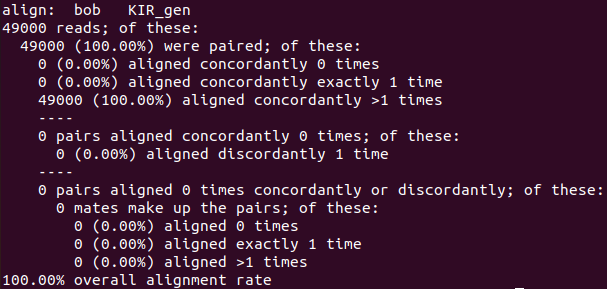
\includegraphics[width=300px]{./img/bob_syntetic_bowtie_align.png}
		\caption{Výpis zarovnání syntetických readů genomu BOB z Bowtie2.}
		\label{fig:bob_syntetic_bowtie_align}
\end{figure}

\begin{figure}[H]		
		\centering
		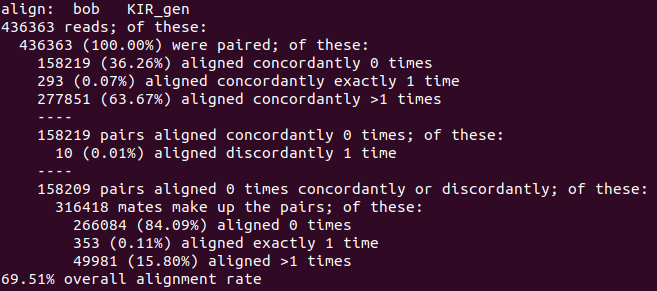
\includegraphics[width=300px]{./img/bob_real_bowtie_align.png}
		\caption{Výpis zarovnání reálných readů genomu BOB z Bowtie2.}
		\label{fig:bob_real_bowtie_align}
\end{figure}

\noindent
Jedním z důvodů, proč se to děje, mohou být chybné báze v reálných readech, které vznikly sekvenováním. V souboru obsahujícím ready je možné nalézt informaci o kvalitě sekvenace jednotlivých bází. V podstatě se jedná o vyjádření toho, jak moc si je sekvenátor jistý danou bází. Kvalita se označuje jako ASCII znak a je rovna ASCII kódu~-~33 (přeskočení netisknutelných znaků). Čím vyšší je ASCII kód, tím je báze kvalitnější. Nejčastěji se hodnota kvality pohybuje mezi 0 a 40, zřídka překročí hodnotu 60. Na následujícím obrázku je zobrazen graf kvality bází vzhledem k pozici v readu.

\begin{figure}[H]		
		\centering
		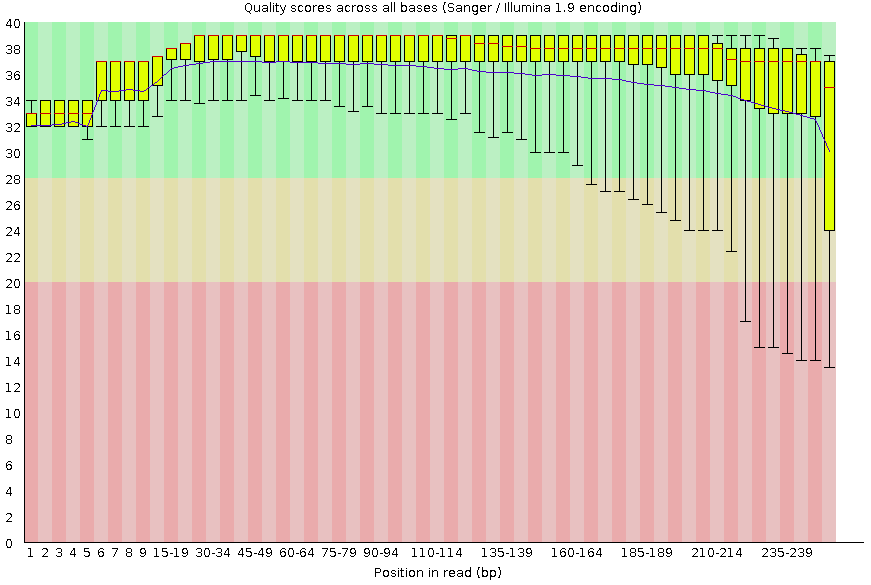
\includegraphics[width=190px]{./img/quality_graf_bob_no_trim_r1.png}
		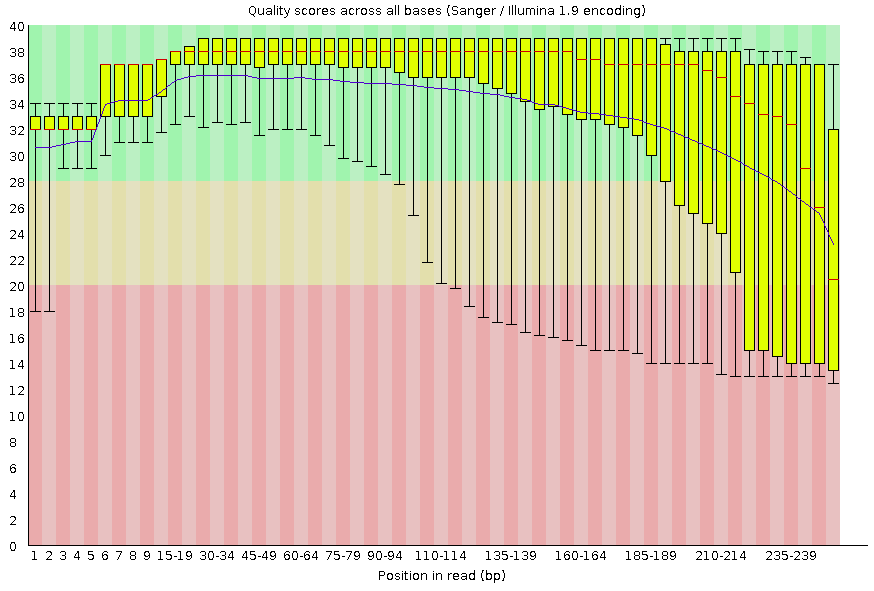
\includegraphics[width=190px]{./img/quality_graf_bob_no_trim_r2.png}
		\caption{Zobrazení kvality dat genomu BOB, v levé části pro první z páru readů a v pravé části pro druhé části readů. V grafu se směrem nahoru zvyšuje kvalita báze. Z leva do prava se pak zvyšuje pozice báze v readu. Je patrné, že čím je pozice v readu vyšší, tím nižší je kvalita báze, a zároveň v druhých párech readů je kvalita znatelně horší.}
		\label{fig:graf_quality_no_trim}
\end{figure}


\noindent
Nabízí se tedy řešení nekvalitní báze na konci readů odstranit. Na odstranění nekvalitních bází byl použit nástroj Trimmomatic 0.38.0 na serveru Galaxy \cite{galaxy}. Na odstranění bylo použito posuvné okénko velikosti 8 s průměrnými kvalitami 15. 


\begin{figure}[H]		
		\centering
		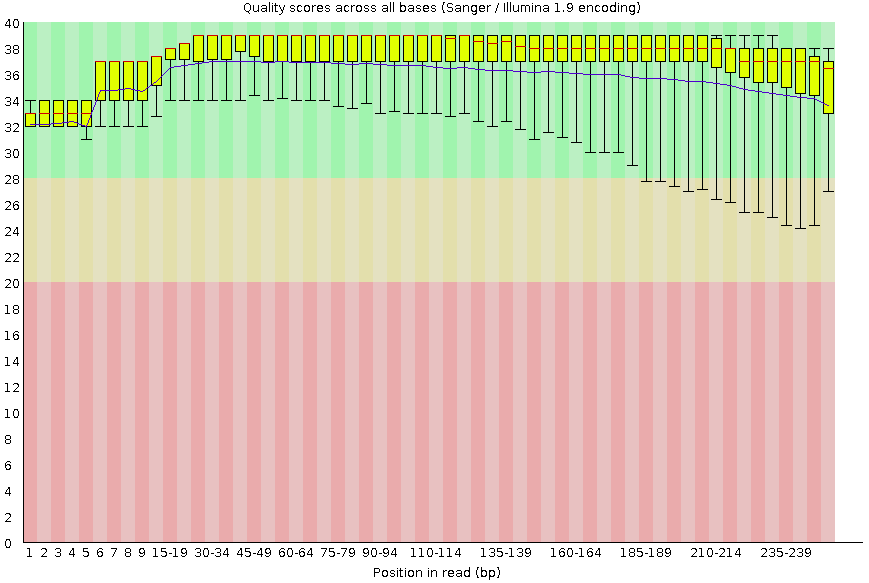
\includegraphics[width=190px]{./img/quality_graf_bob_trim_r1_8_15.png}
		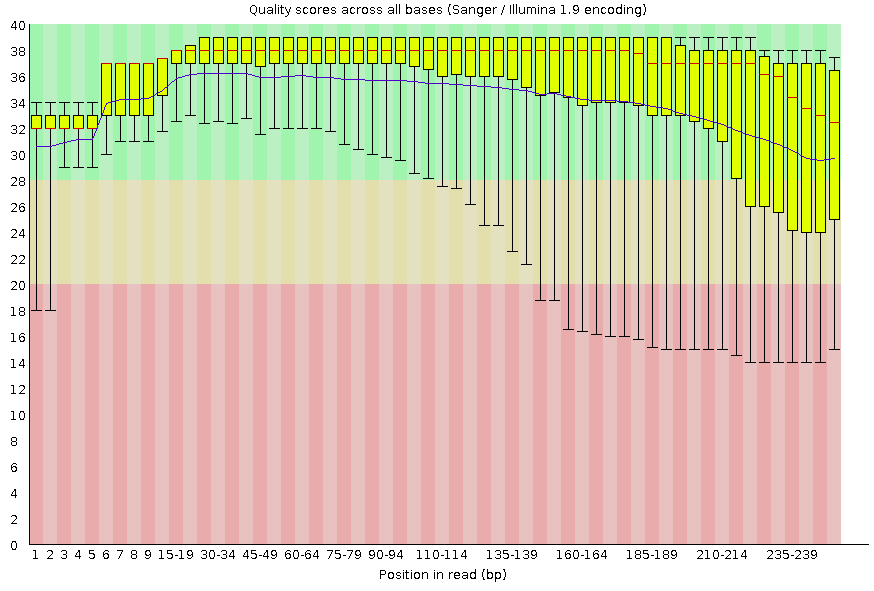
\includegraphics[width=190px]{./img/quality_graf_bob_trim_r2_8_15.png}
		\caption{Zobrazení kvality dat genomu BOB po ořezu nekvalitních bází, v levé části pro první z páru readů a v pravé části pro druhé části readů. V grafu se směrem nahoru zvyšuje kvalita báze. Z leva do prava se pak zvyšuje pozice báze v readu. Je patrné, že čím je pozice v readu vyšší, tím nižší je kvalita báze, a zároveň v druhých párech readů je kvalita znatelně horší.}
		\label{fig:graf_quality_trim}
\end{figure}


\noindent
Následujcí tabulka zobrazuje porovnání výsledků bez ořezu nekvalitních bází a s jejich ořezem. Jak je vidět, nelze jednoznačně říci, že by se výsledky zlepšily.

\begin{center}
\tiny
\rowcolors{2}{gray!25}{white}
\begin{tabular}{l c|| c | c l | c l }
 & & \multicolumn{5}{c}{Krok 4} \\ 
Genom & Alel & \Gape[0pt][2pt]{\makecell[c]{Zbývá \\ alel}} & \multicolumn{2}{c}{Ztraceno} & \multicolumn{2}{|c}{\Gape[0pt][2pt]{\makecell[c]{Geny \\ navíc}}}  \\
\hline
\hline
\Gape[0pt][2pt]{\makecell[l]{amala \\ bez ořezu kvality}} & 19 (0) & 60 & 5 & \Gape[0pt][2pt]{\makecell[l]{2DL2*00301 \\ 2DL3*001 \\ 3DL2*0070102 \\ 3DL2*0020105 \\ 3DP1*00901}} & 2 & \Gape[0pt][2pt]{\makecell[l]{2DL5B \\ 3DL2}} \\ 

\Gape[0pt][2pt]{\makecell[l]{amala \\ s ořezem kvality }} & 19 (0) & 52 & 4 &  \Gape[0pt][2pt]{\makecell[l]{2DL3*001 \\ 2DL2*00301 \\ 3DL2*0070102 \\ 3DP1*00901}}  & 1 &  2DL5B \\ 
\hline
\Gape[0pt][2pt]{\makecell[l]{bob \\ bez ořezu kvality}} & 19 (0) & 52 & 7 & \Gape[0pt][2pt]{\makecell[l]{3DL3*01303 \\ 2DL2*00301 \\ 2DL3*00201 \\ 3DL2*0070102 \\ 3DP1*00302 \\ 2DL4*001 \\ 2DL1*00302}} & 2 & \Gape[0pt][2pt]{\makecell[l]{2DL5B \\ 2DL1}} \\ 

\Gape[0pt][2pt]{\makecell[l]{bob \\ s ořezem kvality }} & 19 (0) & 51 & 7 & \Gape[0pt][2pt]{\makecell[l]{2DL2*00301 \\ 2DL3*00201 \\ 3DL3*01303 \\ 3DL2*0070102 \\ 3DP1*00302 \\ 2DL4*001 \\ 2DL1*00302}} & 3 & \Gape[0pt][2pt]{\makecell[l]{2DL5B \\ 2DS3 \\ 2DL1}} \\ 
\end{tabular}

\label{tab:cut_quality}
\captionof{table}{Porovnání výsledků při odstřižení nekvalitních bází na experimentu 2. Odřezány byly alely, které měly pokrytí menší než 70 \%. Za blízké byly považovány v případě, kdy byla jejich vzdálenost mezi sebou menší než 100. \textit{Alel} u genomu značí počet alel v daném genomu. Číslo v závorkách udává, kolik alel se v daném genomu vyskytuje dvakrát. \textit{Zbývá alel} určuje, kolik alel ještě zůstalo ve výběru, \textit{ztraceno} značí kolik alel má být v genomu, ale algoritmus je vyřadil. Za tímto číslem jsou vypsané alely, které byly ztraceny, \textit{geny navíc} udávají počet a jaké geny již neobsahují žádnou z alel, která náleží do daného genomu. }
\end{center}

\noindent
V následujícím textu přibyde k referenční alele a nástrojem identifikované alele pojem biologická reference. Myslí se tím identifikace alel provedená v laboratoři, odkud pochází komerční linie.
\\
\\
Dodaná reálná data nemají biologickou referenci až na úroveň non-coding regionu. Příkladem může být biologická reference 2DL1*00201 v níže uvedené ukázce biologické reference genomu KAS011. K této alele je možné přířadit až 16 alel z referenčních sekvencí. Díky tomuto problému není možné plnohodnotně posoudit přesnost a úplnost nástroje. Znak $+$ značí přítomnost genu bez bližšího určení alely, tzn. že v některých případech není alela určená vůbec.
\\
\\
\noindent 
Ukázka dodaných identifikací KAS011
\begin{multicols}{2}
\begin{itemize}
	\itemsep0em
	\item 2DL1: 00201, 00302
	\item 2DL2:
	\item 2DL3: +
	\item 2DL4: 00103, 005
	\item 2DL5A: 00101
	\item 2DL5B:
	\item 2DP1: 002, 00301
	\item 2DS1: 00201
	\item 2DS2:
	\item 2DS3:
	\item 2DS4: 00301
	\item 2DS5: 00201
	\item 3DL1: 008
	\item 3DL2: 01001, 019
	\item 3DL3: 00901, 01302
	\item 3DP1: 00302, 006
	\item 3DS1: 01301
\end{itemize}
\end{multicols}

\noindent 
Podrobnější zhodnocení všech verifikačních linií vycházející z identifikace dané úrovně rozlišení je uvedeno v následující kapitole.


\chapter{Zhodnocení z hlediska úrovně rozlišení}
Na následujících dvou grafech jsou zobrazeny všechny zbývající alely genů 2DS1 a 2DL4 u genomu BOB. Jak je vidět z obrázku, u genu 2DS1 je možné určit coding region tzn. prvních pět čísel. Oproti tomu v případě genu 2DL4 to možné není. 


\begin{figure}[H]
	\centering
    \def\svgwidth{\columnwidth}
    \import{svg/}{uroven_rozliseni_syntetic.pdf_tex} 
\end{figure}

\begin{figure}[H]
	\centering
    \def\svgwidth{\columnwidth}
    \import{svg/}{2DL4_uroven_rozliseni.pdf_tex} 
\end{figure}

\noindent
Následující tabulka zobrazuje možnost rozlišení alel u syntetických readů. V případě genu 3DL3 lze jednoznačně prohlásit, že alely od sebe rozlišit nelze. Oproti tomu v případě genu 2DS2 a 3DL3 alely rozlišit lze. 


\begin{center}
\tiny
\rowcolors{2}{gray!25}{white}
\begin{tabular}{l || c | c | c | c | c | c | c | c | c | c | c  }
 & 2DL1 & 2DL4 & 2DS1 & 2DS2 & 2DS4 & 2DS5 & 3DL1 & 3DL2 & 3DL3 & 3DP1 & 3DS1 \\ 
\hline
\hline
amala &  &  &  &  &  &  &  &  & N &  & A - 5 \\ 
bob &  & N & A - 5 & A - 5 &  &  & N &  &  &  &  \\ 
cox &  &  &  &  &  &  & A - 5 & A - 5 & N &  &  \\ 
ho301 &  & A - 3 &  &  &  &  & N &  &  &  &  \\
jvm &  & A - 5 &  &  & N &  &  &  &  &  &  \\
kas011 &  & A - 5 &  &  & A - 5  &  &  &  & N &  &  \\
olga & A - 5 &  &  &  &  &  & N & A - 5 &  &  &  \\
rsh &  &  &  & A - 5 &  &  &  &  &  &  &  \\
wt51 &  &  &  &  &  & N &  &  &  &  &  \\
test1 &  &  &  & A - 5 &  &  & N &  &  &  &  \\
test2 &  &  &  &  &  &  & A - 5 &  &  &  &  \\
test3 &  &  &  &  &  &  & N &  &  &  &  \\
test4 &  &  & A - 5 &  &  &  & A - 5 &  &  &  &  \\
test5 &  &  &  &  &  &  &  &  & N & N &  \\
test6 & N &  &  &  &  &  &  &  & N &  &  \\
test7 & A - 5 & A - 5 &  &  &  &  &  &  & N &  &  \\
test8 &  &  &  & A - 5 &  &  &  &  & N &  &  \\
test9 &  &  &  & A - 5 & A - 5 &  &  &  & N &  &  \\
test10 &  &  &  & A - 5 &  &  & A - 5 &  &  &  &  \\
test11 & &  &  & A - 5 &  &  &  &  &  &  &  \\  
\end{tabular}
\captionof{table}{Zhodnocení zbylých alel v experimentu 2 po 4. kroku z hlediska úrovně rozlišení. Tabulka obsahuje jen alely, které měly ve výsledcích nějakou informaci o úrovni rozlišení. V případě, kdy se v políčku nachází znak $N$, znamená to, že zbylo více alel, přičemž některá z nich nepatřila do genomu. V případě znaku "A" \space  alely rozlišit lze. Za pomlčkou se pak nachází číslo určující úroveň rozlišení, tedy na kolik čísel mají společný základ. }
\end{center}


\noindent
V případě reálných dat není možné úroveň rozlišení jednoduše určit, protože biologická reference není určena až na nejnižší úroveň, jak již bylo uvedeno v předchozí kapitole. Níže je zobrazená tabulka zjednodušeně popisující úroveň rozlišení u reálných dat. U genů 2DL5A, 2DS1, 2DS2 a 2DS3 bylo určení alely minimálně na 3 místa v coding regionu nebo v souladu s biologickou referencí. V případě ostatních genů se vždy vyskytoval alespoň jeden případ, kdy bylo možné alely rozlišit. 

\begin{center}
\tiny
\rowcolors{2}{gray!25}{white}
\begin{tabular}{l || c | c | c | c | c | c | c | c | c}
& amala & bob & cox & ho301 & jvm & kas011 & olga & rsh & wt51  \\
\hline
\hline
2DL1 & NE & NE & 5R & 3R & 5R & 5R & NE & 5R & 0R\\
2DL4 & 3 & 3R & NE & 3 & 5R & 3R & NE & 7R & 5R \\
2DL5A & 3R & 3 & 5R & &  & 5R & 5R & & 5R\\ 
2DL5B &  &  &  & NE & &  & & 4R & \\
2DP1 & 5R & 5R & 5R & 5R & NE & 5R & 5R & 3R & 3R \\
2DS1 & 5R & 5R & 5R & & & 5R & 3R & & 3R\\
2DS2  & 5R & 3R & & 5R & 5R & & & 5R & 5R\\ 
2DS3 & &  & & 5R & & & & & 0R\\
2DS4 & NE & NE & 3R & 3R & 6R & 5R & 3R & 0R &  \\
2DS5 & NE & NE & 5R & & & NE & NE & 6R & NE \\
3DL1 & NE & NE & 5 & 3R & 3R & 3R & NE & 3R &  \\
3DL2 & NE & NE & NE & 5R & 3R & NE & NE & 0R & 0R\\ 
3DL3 & NE & NE & NE & NE & NE & NE & NE & NE & 3R\\
3DP1 & 3R & NE & 3R & 5R & 3R & 3R & NE & 3R & 0R\\
3DS1 & NE & 5R & 3R &  & &  NE & NE & & NE\\


\end{tabular}
\captionof{table}{Zhodnocení zbylých alel u reálných dat v experimentu 2 po 4. kroku z hlediska úrovně rozlišení. Tabulka obsahuje jen alely, které měly ve výsledcích nějakou informaci o úrovni rozlišení. V případě, kdy se v políčku nachází znak $NE$ nebylo možné alelu rozpoznat, ale v biologické referenci byla uvedena. V případě čísla značí, na jak velkou přesnost byla alela určena. R za tímto číslem značí, že tato úroveň rozlišení byla uvedena i v biologické referenci. Pokud je políčko prázdné, gen se v genomu nenachází nebo byl ztracen.}
\end{center}
 
\noindent
Ať už z důvodu nezarovnání všech reálných readů, možné přítomností alely, pro kterou není referenční sekvence, či kvůli jiné z výše uvedených příčin, jsou tyto výsledky očekávané.


\chapter{Závěr}
Práce se zabývá návrhem nástroje pro automatickou identifikaci KIR alel. Identifikace KIR alel je využitelná při transplantaci krvetvorných buněk, kdy se rozhoduje mezi více dárci shodnými v HLA znacích. Zvolení dárce s vhodnějšími KIR geny snižuje riziko relapsu (návratu nemoci).
\\
\\
Toto téma je stále aktuální. Zatím je prokázán vliv jen KIR genů, resp. jejich haplotypových kombinací. V současné době se zkoumá také vliv alelických variant, jelikož doposud bylo prokázáno, že některé formy genů se neexprimují, tzn. gen se sice v genomu nachází, ale není z něj vytvořen žádný produkt na povrchu buňky a tak nemá jak vyvolat či ovlivnit jakoukoliv reakci v organismu \cite{exprimace_zaver}. Z biologického hlediska je důležitá právě exprimace, která je závislá jen na coding-regionu. Tudíž z praktického hlediska stačí, aby nástroj byl schopný určit alelu na coding úroveň, tedy prvních pět čísel alely. 
\\
\\
V teoretické části byly popsány a rozbrány geny, především non-HLA gen Killer-cell immunoglobulin-like receptor (KIR), a jejich vliv na transplantaci krvetvorných buněk. Dále byly představeny natural killer buňky a jejich funkce v rámci imunitního systému. Pro zjištění typizace HLA a KIR slouží sekvenační metody, které byly shrnuty a popsány. Konkrétněji Sanger sekvenování a next-generation sequencing (NGS). V neposlední řadě byly analyzovány bioinformatické nástroje pro zpracování NGS dat se zaměřením na generátor syntetických readů ART a zarovnávač NGS readů Bowtie2.
\\
\\
V realizační části bylo navrženo a implementováno prototypové řešení v jazyce Python za pomocí knihovny pysam pro identifikaci KIR alel. Jazyk Python byl zvolen z důvodu jednoduchého použití, díky čemuž nebyl vývoj časově náročný. Parametry nástroje ART byly určeny tak, aby výstupní ready co nejvíce odpovídaly datům získaným z FN Plzeň/BC LF UK Plzeň. Během práce bylo implementováno a vyzkoušeno několik přístupů, které byly v práci zhodnoceny. Největší překážkou je podobnost alel. Alely mohou být dlouhé až 16 000 bp (nukleových bází). Ready ze sekvenátoru jsou ovšem dlouhé 250 bp. Vzhledem k podobnosti alel (u některých dokonce jen jedna nukleová báze) není žádnou výjimkou, že read je zarovnán na alelu, ke které nepatří. 
\\
\\
Nástroj byl implementován a laděn na syntetických readech. Následná verifikace byla provedena na komerčních buněčných liniích sekvenovaných ve FN Plzeň/BC LF UK Plzeň. Verifikace nástroje na reálných datech odpovídala očekávaným předpokladům. Rozdíl reálných readů od syntetických byl už v jejich zarovnání, kdy v případě reálných dat bylo zarovnáno kolem 70 \% readů, oproti tomu v případě syntetických readů byly zarovnány všechny. V rámci návrhu nástroje a provedených experimentů byly identifikovány základní slabiny automatické identifikace KIR alel, a sice že reálná data nejsou vždy identifikovaná až na úroveň non-coding region, protože z biologického hlediska není v některých případech možné určit alelu na nejnižší známou úroveň, či označení, že se zde gen nachází, ale ani zmínka o tom, o jakou alelu by se mohlo jednat. Tyto problémy souvisejí i se zhodnocením z hlediska úrovně rozlišení, kde u reálných dat v případě biologické reference pouze na coding region vyjde více alel na non-coding region se stejným zákládem codingu regionu. Kromě toho je v reálných datech možné narazit na alelu, která se mezi referenčními sekvencemi nenachází. Nyní je známo 1109 alel, přičemž existuje referenční sekvence pouze pro 461 alel.
\\
\\
Do budoucna se nabízí zamyslet se více nad efektivním vytvořením clusterů, kde by se zohledňovala délka readů. V případě verifikace by bylo vhodné více probádat kvalitu dat a odstřihávání nekvalitních bází. 


\chapter{Výkladový slovník pojmů a zkratek}

\begin{labeling}{alligator}
	\item [WHO] World health organization, světová zdravotnická organizace
	\item [ČNRDD] Český národní registr dárců kostní dřeně
	\item [MHC] Major histocompatibility complex, genetický systém	
	\item [HLA] Human leucocyte antigen, podskupina MHC
	\item [KIR] Killer imunoglobilin like-receptor, skupina genů
	\item [NK] Natural killer, buňka imunitního systému
	\item [DNA] Deoxyribonukleová kyselina; dvoušroubovice, která obsahuje páry bází C, G, A, T 
	\item [RNA] Ribonuklové kyselina; obsahuje báze C, G, A, U; šablona přímo pro vytvoření proteinů; hlavní funkcí zajištění překladu DNA do struktury proteinů (DNA -> mRNA -> rRNA -> tRNA -> RNA) 
	\item [Báze] nukleové báze; A - Adenin, C - Cytosin, G - Guanin, T - Thymin
	\item [bp] base pair; jeden z párů A - T nebo C - G
	\item [kb] kilobase 1 kb = 1000 bp
	\item [ART] nástroj na vytváření syntetických readů
	\item [Bowtie] nástroj na zarovnání readů proti referenčním genům
	\item [SAM] Sequence Alignment/Map; Formát souboru na uložení zarovnání
	\item [BAM] Binární verze souboru SAM
\end{labeling}


% 
% PRO ANGLICKOU SAZBU JE NUTNÉ ZMĚNIT
% CITAČNÍ STYL!
%
\nocite{*}
\bibliographystyle{csplainnatkiv}
{\raggedright\small
\bibliography{literatura}
}


\appendix
\chapter{Uživatelská dokumentace}
Ke spuštění programu je třeba mít nainstalovaný:
\begin{itemize}
\item ART ve verzi MountRainier
\item Bowtie2 ve verzi 2.4.1
\item Python ve verzi 3.8
\item Python knihovny 
	\begin{itemize}
		\item pysam 
		\item python-Levenshtein
		\item matplotlib
		\item numpy
	\end{itemize}
\end{itemize}

\noindent
Doporučený operační systém je Linux, na Windows se mohou vyskytnout problémy s knihovnou htslib. 

\section{Získání potřebného softwaru}
\textbf{Python knihovny a moduly} \\
Knihovny a moduly je možné získat pomocí PyPi.
\begin{itemize}
	\item \colorbox{gray!15}{\textit{pip install pysam}}
	\item \colorbox{gray!15}{\textit{pip install python-Levenshtein}}
	\item \colorbox{gray!15}{\textit{pip install matplotlib}}
	\item \colorbox{gray!15}{\textit{pip install numpy}}
\end{itemize}

\noindent
Jinou možností je použít oficiální návody uvedené pro knihovnu pysam na \cite{pysam}, knihovnu python-Levenshtein \cite{python_leve}, matplotlib \cite{matplotlib} a numpy \cite{numpy}.
\\
\\
\textbf{ART}\\
Nástroj ART slouží ke generování syntetických readů. Odkaz na stažení nástroje u oficiálního článku \cite{art} je bohužel nefunkční. Je možné využít tento zdroj \cite{art_download}. V případě, že bude i tento link nefunkční je možné nástroj vyhledat na stejné stránce po zadání textu \textit{ART} do vyhledávácího pole, typicky první výsledek \textit{ART - Set of simulation tools ... }
\\
\\
Práce je odzkoušená s verzí MountRainer. Ve staženém archivu se nachází několik souborů \textit{README}. Pro tuto práci je důležitý soubor \textit{art\_illumina\_\\README.txt}, který obsahuje návod na instalaci nástroje a vysvětlení parametrů.  
\\
\\
Parametry shodující se s parametry dat získaných z FN Plzeň/BC LF UK Plzeň jsou paired end ready dlouhé 250 bp, profil sekvenátoru MSv1, s nakopírování sekvencí 100. Všechny tyto parametry jsou již nastavené ve skriptu.
\\
\\
\textbf{Bowtie2}\\
Bowtie2 slouží k zarovnání readů na refrenční sekvenci a je dostupný na \cite{bowtie2_download}. Práce je odzkoušená s verzí 2.4.1. Ve stažené verzi je manuál s potřebnými instrukcemi. Stejně tak je na stránkách Bowtie2 sekce Getting started. 

\section{Získání referenčních sekvencí}
\label{sec:ref_sek}
Referenční soubory \textit{\_gen.fa} a \textit{\_nuc.fa} použité v práci jsou k nalezení na CD ve složce \textit{prilozena data/referencni sekvence}. Případně nejnovější verzi je možné získat na IPD-KIR \cite{imgt_hla_database} v záložce \textit{KIR}, dále v pravém menu \textit{GitRepos} složka \textit{fasta}.

\section{Nastavení programu}
Veškeré nastavení aplikace probíhá pomocí souboru \textit{config.py}
\\
\\
\noindent
Parametry configu:
\begin{itemize}
	\item CREATE\_READS - Značí, zda má být spuštěn modul vytvoření syntetických readů. Očekávaný hodnota je True nebo False.
	\item ALIGN - Značí, zda má být spuštěn modul pro zarovnání readů vzhledem k referenčním genům. Očekávaná hodnota je True nebo False.
	\item IDENTIFY - Značí, zda má být spuštěna identifikace alel. Očekávaná hodnota je True nebo False.
	\item PRECOMPUTATION\_DISTANCE - Předpočítání vzájemné vzdálenosti mezi jednotlivými alelami do pyc souboru. 
	\item EXP1 - Značí, zdá má být spuštěn experiment 1 pro identifikaci.
	\item EXP2 - Značí, zdá má být spuštěn experiment 2 pro identifikaci.
	\item EXP3 - Značí, zdá má být spuštěn experiment 3 pro identifikaci.
	\item PATH\_TO\_DATA\_FOLDER - Značí cestu ke složce s daty. Dá se využít v případě, kdy adresářová struktura odpovídá struktuře navržené níže.
	\item REFERENCE\_KIR\_GENS\_FILE - Soubor se všemi referenčními geny. 
	\item GENOME\_FOLDER - Označuje cestu složky, do které jsou ukládány vytvořené genomy. 
	\item GENOMES - Slovník, který definuje genomy podle obsahů genů. Na základě toho budou vytvořeny genomy.
	\item BOWTIE\_HOME\_DIRECTORY - Označuje cestu ke nástroji Bowtie.
	\item READS\_FOLDER - Označuje složku, do které budou ukládány ready. Případně z které budou načítány.
	\item BOWTIE\_INDEX\_FOLDER - Označuje složku, do které budou ukládány indexy z Bowtie. Případně z které budou načítány. 
	\item BOWTIE\_BUILD\_INDEX - Značí zda mají být vytvořeny Bowtie indexy. Pokud bude hodnota nastavena na False, musí být přítomny indexy z minulého běhu, jinak zarovnávání nebude fungovat. Očekávaná hodnota je True nebo False. (Pro první běh je typická hodnota True)
	\item BOWTIE\_THREADS - Počet vláken na která má být Bowtie spuštěn.	
	\item ALIGNMENT\_FOLDER - Označuje složku, do které budou ukládány zarovnané ready. Případně z které budou načítány. 
	\item BAM\_FOLDER - Označuje složku na uložení BAM souborů.  
	\item RESULT\_FOLDER - Označuje složku, do které budou uloženy výsledky vyhodnocení.
	\item ALELS\_STATISTICS\_FOLDER - Označuje složku, do které budou uloženy statistiky mezivýsledků.
	\item TEMP\_FOLDER - Složka, kam se budou ukládat soubory, které jsou potřeba jen pro mezizpracovávání, jako jsou bowtie indexy při mnohonásobném zarovnávání u experimentu 2 a experimentu  3.
	\item REFERENCE\_FOLDER - Složka kam se ukládají nově vytvořené reference z experimentů.
	\item ALELS\_DISTANCE\_FILE\_PYC - Soubor do kterého se budou ukládat předpočítané vzdálenosti mezi jednotlivými alelami. 
	\item LEVENSHTEIN\_DISTANCE\_CUT - Tato hodnota udává, do jak vysoké hodnoty bude věnována pozornost vzdálenosti mezi jednotlivými alelami a které vzdálenosti tedy budou ukládány. Je to především z důvodu paměťové náročnosti.
	\item CUT\_COVERAGE\_ALLELES - Hodnota určující minimální procentuální pokrytí alel, které mají být zachovány ve výsledcích.
	 \item CLOSE\_DISTANCE - Hodnota určující do jaké vzdálenosti jsou dvě alely považovány za blízké.
	 \item CLUSTER\_DISTANCE - Hodnota určující maximální vzdálenost alel, které spolu budou sloučeny do clusteru.
\end{itemize}



\section{Doporučená adresářová struktura pro data}
\begin{itemize}
	\item data
		\begin{itemize}
			\item alignments
			\item bam
			\item bowtie\_index
			\item genome
			\item reads
			\item reference			
			\item result
			\item statistics 
			\item temp
		\end{itemize}
\end{itemize}

\section{Spuštění programu}
Program je možné spustit z příkazové řádky pomocí příkazu: 

\begin{itemize}
 \item \colorbox{gray!15}{\textit{python run.py}}
\end{itemize}

\noindent
Podmínkou fungování tohoto postupu je, že je třeba se nacházet v umístění skriptu. 

\section{Výstupy programu}
V případě tvorby vlastních genomů s doporučenou adresářovou strukturou najdeme ve složce \textit{genome} soubory s příponou \textit{.fa}. Každý soubor obsahuje jeden genom.
Vytvořené ready se budou nacházet ve složce reads. Protože genomy jsou paired-end, náleží každému genomu dva soubory s příponou \textit{.fq}. Jeden s \textit{1} na konci a druhý s \textit{2} na konci. 
V případě zarovnání mohou být výstupní soubory indexy ve složce \textit{bowtie\_index}. Kdy pro každý referenční soubor je vytvořeno 6 souborů s příponou \textit{bt2}. Výsledné zarování se pak nachází ve složce \textit{alignments} ve formátu \textit{.sam}. 

\subsection{Výsledky}
Výsledky samotné identifikace je možné nalézt ve složece \textit{result} ve formátu \textit{.txt}. Mezivýsledky jednotlivých kroků experimentů jsou uloženy ve složce statistics a je možné si je prohlédnout pomocí přiloženého skriptu \textit{analysis\_after\_align.py}, který bude popsán níže. Soubor mezivýsledků může vypadat následovně $amala\_KIR\_GEN\_exp2\_step1.pyc$.  Označení začíná názvem genomu - amala, KIR\_GEN značí referenční sekvenci, exp2 udává o který experiment se jedná, step1 určuje ke kterému kroku mezi výsledky patří. 



\section{Analýza referenčních genů}
K analyzování referenčních genů slouží skript \textit{analysis\_alels.py} nacházející se na CD ve složce \textit{software/analysis}. V horní části skriptu je třeba nastavit příslušné cesty.


\begin{itemize}
	\item NUC\_FILE - Soubor z referencí \textit{\_nuc.fa}. Slouží pro porovnání se souborem \textit{\_gen.fa}
	\item GEN\_FILE - Soubor s referenčními sekvencemi.
	\item DISTANCE\_FILE\_PYC - Soubor obsahující všechny vzdálenosti a který bude vytvořen na začátku skriptu.
	\item PLOT\_OUTPUT\_FOLDER - Složka udávající kam se budou ukládat výsledné grafy.
	\item COUNT\_LEVENHSTEIN - Předpočítá vzdálenosti mezi alelami. Využitelné především při opakovaných bězích se stejnou referencí. Při nastavení hodnoty na True je výpočet velmi pomalý.
\end{itemize}

\noindent
Získání referenčních souborů \textit{\_gen.fa} a \textit{\_nuc.fa}, které byly použity v práci, je popsáno v sekci  \hyperref[sec:ref_sek]{Získání referenčních sekvencí.}

\subsection{Spuštění}
Analýzu referenčních genů je možné spustit z příkazové řádky pomocí příkazu:
\begin{itemize}
 \item \colorbox{gray!15}{\textit{python analysis\_alels.py}}
\end{itemize}

\noindent
Podmínkou fungování tohoto postupu je, že je třeba se nacházet v umístění skriptu. 

\subsection{Výstupy programu}
Výstupem analýzy jsou grafy vzdáleností mezi jednotlivými alelami uložených ve složce \textit{PLOT\_OUTPUT\_FOLDER} a jednoduchá statistika, která je zobrazena na následujícím obrázku. \textit{count\_gen} označuje celkový počet alel v souboru \textit{GEN\_FILE}, \textit{count\_nuc} označuje počet alel v souboru \textit{NUC\_FILE}, \textit{match} značí kolik alel je shodných v soubouru \textit{GEN\_FILE} a \textit{NUC\_FILE}, \textit{key not found} značí kolik alel se vyskytuje jen v jenom ze souborů \textit{GEN\_FILE} a \textit{NUC\_FILE}, \textit{something\_wrong} značí nesoulad mezi označením alel podle obsahu a podle pořadového čísla nalezení mezi soubory \textit{NUC\_FILE} a \textit{GEN\_ \\ FILE}. Na druhém řádku \textit{max} značí největší vzdálenost mezi alelami, \textit{min} značí nejmenší vzdálenost mezi alelami, \textit{average distance} značí průměrnou vzdálenost mezi alelami, \textit{median} značí median vzdáleností mezi alelami.

\begin{figure}[H]		
		\centering
		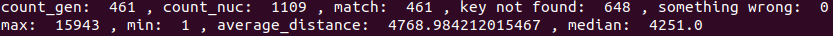
\includegraphics[width=\textwidth]{./img/vystup_analyzy_refrence.png}
		\caption{Zobrazení výstupu ze skriptu \textit{analysis\_alels.py} }
		\label{fig:alels_distance_skript}
\end{figure}

\begin{figure}[H]
    \centering
    \def\svgwidth{\columnwidth}
    \import{svg/}{2DL4cross_gens.pdf_tex} 
    \caption{Ukázka výstupního grafu z analýzy referenčních genů}
\end{figure}

\begin{figure}[H]
    \centering
    \def\svgwidth{\columnwidth}
    \import{svg/}{2DL4_gen.pdf_tex} 
    \caption{Ukázka výstupního grafu z analýzy referenčních genů}
\end{figure}


\section{Analyzování experimentů}
Pro analyzování kroků jednotlivých experimentů je možné využít skript \textit{analysis\_after\_align\_auto.py} nacházející se na CD ve složce \textit{software/analysis}. V horní části skriptu je třeba nastavit příslušné cesty. 

\begin{itemize}
	\item GEN\_FILE - Soubor s referenčními alelami.
	\item ALELS\_STATISTICS\_PYC\_FOLDER - Složka s pyc soubory obsahující statistiku jednotlivých kroků. Typickým příkladem tohoto souboru může být \textit{amala\_KIR\_gen\_exp1\_step1.pyc}.
	\item ALELS\_STATISTICS\_PYC\_REFERENCE\_NAME - Jméno reference, toto je jeden z parametrů, ze kterých se skládá název souborů ze statistics.
	\item ALELS\_STATISTICS\_PYC\_EXPERIMENT - Jméno experimentu, typické hodnoty: exp1, exp2 a exp3
	\item STEPS - Kroky, které se mají analyzovat, typické hodnoty: step1, step2, step3 a step4
	\item STEPS\_LATECH\_TABLE  - Určuje, které kroky se mají vygenerovat do latex tabulky
	\item PLOT\_OUTPUT\_FOLDER - Složka udávající kam se budou ukládat výsledné grafy.
	\item GENOMES\_LIST - Výpis genomů, které mají být analyzovány.
	\item GENOMES\_ALLELES  - Slovník referenčních odpovědí.
\end{itemize}

\subsection{Spuštění}
Analýzu je možné spustit z příkazové řádky pomocí příkazu:
\begin{itemize}
 \item \colorbox{gray!15}{\textit{python analysis\_after\_align\_auto.py}}
\end{itemize}
\noindent
Podmínkou fungování tohoto postupu je, že je třeba se nacházet v umístění skriptu. 

\subsection{Výstupy programu}
Výstupem jsou grafy pokrytí jednotlivých alel uložených ve složce \textit{PLOT\_OUT\\PUT\_FOLDER}, roztříděných podle genů, kroku a genomu.





\section{Používané soubory}

\textbf{Fastq a fq}
\\
\noindent
Soubory s příponou \textit{.fastq} nebo \textit{.fq} obsahují ready a jsou typickým výstupním souborem ze sekvenátoru. V těchto souborech je mimo jiné pro každou bázi vyznačena i kvalita dané báze. Dá se říci, že to vyjadřuje jak si je sekvenátor jistý danou bázi. Kvalita se označuje jako ASCII znak. Kvalita je pak rovna ASCII kodu -33 (přeskočení netisknutelných znaků). Čím vyšší je ASCII kód, tím je báze kvalitnější. Nejčastější kvalita je od 0 do 40, zřídka překročí hodnotu 60. Pro paired end ready jsou vytvořeny vždy dva soubory, jeden s prvními z párů readu a druhý soubor s druhými z párů readů. 
\\
\\
\textbf{SAM}	   
\\
\noindent 
Soubor s příponou \textit{.sam} obsahuje výsledky zarovnání readů.



\chapter{Testovací genomy}
\begin{center}
\tiny
\begin{tabular}{ |c|c|c|c| }
\hline
\textbf{Test1} & \textbf{Test2} & \textbf{Test3} & \textbf{Test4} \\ \hline
	\Gape[0pt][2pt]{\makecell[l]{
3DL3: 0030101, 0140201 \\
2DS2: 0010104 \\
2DL2: 0030105 \\
2DL3: 0020101 \\
2DL5B: 01301 \\
2DS3: 0020102 (2x) \\
2DP1: 0030101, 0010203 \\
2DL1: 0030203, 007 \\
3DP1: 004 (2x) \\
2DL4: 0080104, 010 \\
3DL1: 0150101 \\
3DS1: 014 \\
2DL5A: 00102 \\
2DS5: \\
2DS1: 0020104 \\
2DS4: 0010103 \\
3DL2: 00501 (2x) \\
	}}
&
	\Gape[0pt][2pt]{\makecell[l]{
3DL3: 0090102, 019 \\
2DS2: \\
2DL2: 0010101 \\
2DL3: 0010111 \\
2DL5B: 0020101 \\
2DS3:  \\
2DP1: 0020107, 0030102 \\
2DL1: 0020102, 0030210 \\
3DP1: 004, 01001 \\
2DL4: 0080104 (2x) \\
3DL1: 0070101 \\
3DS1: 078 \\
2DL5A: 0050101 \\
2DS5: 010 \\
2DS1: 0020102 \\
2DS4:0010103 \\
3DL2: 0020101, 00501
}}
&
	\Gape[0pt][2pt]{\makecell[l]{
3DL3: 005, 0140201 \\
2DS2: \\
2DL2:  \\
2DL3: 0010101, 0020103 \\
2DL5B:  \\
2DS3:  \\
2DP1: 0020108 (2x) \\
2DL1: 0040101, 008 \\
3DP1: 0030102, 00902 \\
2DL4: 0010306, 0050104 \\
3DL1: 002, 0040101 \\
3DS1:  \\
2DL5A: \\
2DS5: \\
2DS1: \\
2DS4: \\
3DL2: 0010301, 008
}}
& 
	\Gape[0pt][2pt]{\makecell[l]{
3DL3: 0030104, 007 \\
2DS2: 0010105 \\
2DL2: 0030101 \\
2DL3: 0010102 \\
2DL5B:  \\
2DS3:  \\
2DP1: 008 \\
2DL1: 007 \\
3DP1: 007, 00902 \\
2DL4: 0010307, 0080104 \\
3DL1: 0150202 \\
3DS1: 055 \\
2DL5A: \\
2DS5: 007 \\
2DS1: 0020101 \\
2DS4: 0060101 \\
3DL2: 0020101, 00903
	}}
\\
\hline

\textbf{Test5} & \textbf{Test6} & \textbf{Test7} & \textbf{Test8}\\ \hline
	\Gape[0pt][2pt]{\makecell[l]{
3DL3: 0140202, 036 \\
2DS2: \\
2DL2:  \\
2DL3: 0010109, 006 \\
2DL5B:  \\
2DS3: 0010301 \\
2DP1: 0030102, 009 \\
2DL1: 0030208, 00303 \\
3DP1: 001, 002 \\
2DL4: 0010202 (2x) \\
3DL1:  0200101 \\
3DS1: 0130102 \\
2DL5A: 0010102 \\
2DS5:  \\
2DS1: 0020105 \\
2DS4: \\
3DL2: 00202, 018 \\	
	}}	
&
	\Gape[0pt][2pt]{\makecell[l]{
3DL3: 0090102, 0140203 \\
2DS2: 0010111 \\
2DL2: 0010105 \\
2DL3: 0010102 \\
2DL5B: 0080101 \\
2DS3: 0010302 \\
2DP1: 0020103, 010 \\
2DL1: 0030203, 0040102 \\
3DP1: 0030202, 0030402 \\
2DL4: 0010303, 00901 \\
3DL1: 0050102, 0250102 \\
3DS1:  \\
2DL5A: \\
2DS5: \\
2DS1:  \\
2DS4: 0010104, 010 \\
3DL2: 0010302, 01001	 \\
	}}
&
	\Gape[0pt][2pt]{\makecell[l]{
3DL3: 00802,0090103 \\
2DS2: \\
2DL2:  \\
2DL3: 0010103,0010108 \\
2DL5B: \\
2DS3:  \\
2DP1: 0020106, 004 \\
2DL1: 0030204, 0030205 \\
3DP1: 0030202 (2x) \\
2DL4: 0010201, 0010305 \\
3DL1: 008, 0150203 \\
3DS1:  \\
2DL5A: \\
2DS5: \\
2DS1: \\ 
2DS4: 0010107, 0030104 \\
3DL2: 0020105, 00901 \\
	}}
&
	\Gape[0pt][2pt]{\makecell[l]{
3DL3: 0030103, 00601 \\
2DS2: 0010103, 0010112 \\
2DL2: 0010102, 0030101 \\
2DL3:  \\
2DL5B: 0070101 \\
2DS3: 0020101 (2x), 0010302 \\
2DP1: 0030102 \\
2DL1: 00402 \\
3DP1: 0030101, 005 \\
2DL4: 00104, 0080104 \\
3DL1:  \\
3DS1: 0130104, 055 \\
2DL5A: 0050102 (2x) \\
2DS5:  \\
2DS1: 0020102, 0020105 \\
2DS4: \\
3DL2: 0010102, 0070102 \\
}}	 
\\
\hline

\textbf{Test9} & \textbf{Test10} & \textbf{Test11} & \\ \hline
	\Gape[0pt][2pt]{\makecell[l]{	
3DL3: 0030103,00601 \\
2DS2: 0010103, 0010112 \\
2DL2: 0010102, 0030101 \\
2DL3: \\
2DL5B: 0070101 \\
2DS3: 0020101 (2x) \\
2DP1: 0030102 \\
2DL1: 00402 \\
3DP1: 0030101, 005 \\
2DL4: 00104, 0080104 \\
3DL1: 0150208 \\
3DS1: 0130104 \\
2DL5A: 01201 \\
2DS5: \\
2DS1: 0020102 \\
2DS4: 0040101 \\
3DL2: 0010102, 0070102 \\
	}}	
&
	\Gape[0pt][2pt]{\makecell[l]{
3DL3: 0030101, 0140201 \\
2DS2: 0010104 \\
2DL2: 0030105 \\
2DL3: 0020101 \\
2DL5B: 01301 \\
2DS3: 0020102 (2x) \\
2DP1: 0010203, 0030101 \\
2DL1: 0030203, 007 \\
3DP1: 004 (2x) \\
2DL4: 0080104, 010 \\
3DL1: 0150101 \\
3DS1: 014 \\
2DL5A: \\
2DS5:  \\
2DS1: 0020104 \\
2DS4: \\
3DL2: 00501 (2x) \\
	}}	
&
	\Gape[0pt][2pt]{\makecell[l]{
3DL3: 0030103, 00601  \\
2DS2: 0010103, 0010112 \\
2DL2: 0010102, 0030101 \\
2DL3:  \\
2DL5B:  \\
2DS3:  \\
2DP1: 0030102, 008 \\
2DL1: 00402 (2x) \\
3DP1: 0030101, 005 \\
2DL4: 00104, 0080104 \\
3DL1:  \\
3DS1: 0130104, 055 \\
2DL5A: 0050102 (2x) \\
2DS5: 0020102, 0020103 \\
2DS1: 0020102, 0020105 \\
2DS4: \\
3DL2: 0010102, 0070102 \\	
	}}
&
	
\\
\hline
\end{tabular}
\label{tabulka:rf1}
\end{center}

\begin{center}
\tiny
\begin{tabular}{ |c|c|c|c| }
\hline
\textbf{AMALA} & \textbf{BOB} & \textbf{COX} & \textbf{HO301} \\ \hline
	\Gape[0pt][2pt]{\makecell[l]{
3DL3: 0040201, 00802  \\
2DS2: 0010101 \\
2DL2: 0030102 \\
2DL3: 0010109 \\
2DL5B:  \\
2DS3:  \\
2DP1: 0020108 \\
2DL1: 0030201 \\
3DP1: 007, 0090101 \\
2DL4: 0010201, 0050106 \\
3DL1: 0150201 \\
3DS1: 0130101 \\
2DL5A: 00102 \\
2DS5: 0020101 \\
2DS1: 0020106 \\
2DS4: 0010101 \\
3DL2: 0020105, 0070102 \\
	}}
&
	\Gape[0pt][2pt]{\makecell[l]{
3DL3: 00101, 019  \\
2DS2: 0010104 \\
2DL2: 0030101 \\
2DL3: 0020102  \\
2DL5B:  \\
2DS3:  \\
2DP1: 0030101 \\
2DL1: 0030210 \\
3DP1: 002, 0030203 \\
2DL4: 0010202, 0050101 \\
3DL1: 002  \\
3DS1: 0130105 \\
2DL5A: 0010101 \\
2DS5: 0020104 \\
2DS1: 0020101 \\
2DS4: 0010105 \\
3DL2: 0020101, 0070102 \\
	}}
&
	\Gape[0pt][2pt]{\makecell[l]{
3DL3: 00102, 0090101  \\
2DS2: \\
2DL2:  \\
2DL3: 0020101, 006 \\
2DL5B:  \\
2DS3:  \\
2DP1: 0030102 (2x) \\
2DL1: 0020102 (2x) \\
3DP1: 005, 006 \\
2DL4: 0050102, 00901 \\
3DL1: 0050103 \\
3DS1: 055 \\
2DL5A:  \\
2DS5: 0020102 \\
2DS1: 0020105 \\
2DS4: 010 \\
3DL2: 0010301, 0070103 \\
	}}
&
	\Gape[0pt][2pt]{\makecell[l]{
3DL3: 00102, 0090101  \\
2DS2: \\
2DL2:  \\
2DL3: 0020101, 006 \\
2DL5B:  \\
2DS3:  \\
2DP1: 0030102 (2x) \\
2DL1: 0020102 (2x) \\
3DP1: 005, 006 \\
2DL4: 00501, 00901 \\
3DL1: 0050103 \\
3DS1: 055 \\
2DL5A:  \\
2DS5: 0020102 \\
2DS1: 0020105 \\
2DS4: 010 \\
3DL2: 0010301, 0070103 \\
	}}
\\ \hline
\textbf{JVM} & \textbf{KAS011} & \textbf{OLGA} & \textbf{RSH} \\ \hline
	\Gape[0pt][2pt]{\makecell[l]{
3DL3: 00801, 0140201 \\
2DS2: 0010110 \\
2DL2: 0030102 \\
2DL3: 010 \\
2DL5B:  \\
2DS3:  \\
2DP1: 004 \\
2DL1: 0030203 \\
3DP1: 001, 0030202 \\
2DL4: 0010304, 0080101 \\
3DL1: 0010104, 008 \\
3DS1:  \\
2DL5A: \\
2DS5: \\
2DS1:  \\
2DS4: 0030103 (2x) \\
3DL2: 0010101, 018	\\
	}}
&
	\Gape[0pt][2pt]{\makecell[l]{
3DL3: 0090101, 0140203 \\
2DS2:  \\
2DL2:  \\
2DL3: 0020103 (2x) \\
2DL5B:  \\
2DS3:  \\
2DP1: 0020104, 0030101 \\
2DL1: 0020101, 0030209 \\
3DP1: 0030206, 009 \\
2DL4: 0010301, 0050107 \\
3DL1: 008 \\
3DS1: 013011 \\
2DL5A: 0010102 \\
2DS5: 0020101 \\
2DS1: 0020101 \\
2DS4: 0030101 \\
3DL2:01001, 018 \\
	}}
&
	\Gape[0pt][2pt]{\makecell[l]{
3DL3: 00201, 00202  \\
2DS2: \\
2DL2:  \\
2DL3: 0010105 (2x) \\
2DL5B:  \\
2DS3:  \\
2DP1: 0020105, 006 \\
2DL1: 0030204 (2x) \\
3DP1: 0030201 (2x) \\
2DL4: 0050103, 00901 \\
3DL1: 0010102, 0050101 \\
3DS1: 0130107 \\
2DL5A: 00103 \\
2DS5: 0020103 \\
2DS1: 0020101 \\
2DS4: 010 \\
3DL2: 0070101, 0070102 \\
	}}
&
	\Gape[0pt][2pt]{\makecell[l]{
3DL3: 00202, 0040202 \\
2DS2: 0010108 \\
2DL2: 0030104 \\
2DL3: 0010107 \\
2DL5B: 004 \\
2DS3:  \\
2DP1: 0020110, 009 \\
2DL1: 0030205, 01201 \\
3DP1: 0030401, 008 \\
2DL4: 0010307, 00901 \\
3DL1: 0050101, 01701 \\
3DS1: \\
2DL5A:  \\
2DS5: 006 \\
2DS1:  \\
2DS4: 0060102 \\
3DL2: 023, 056	 \\
	}}
\\
\hline
\textbf{WT51} &  &  &  \\ \hline
	\Gape[0pt][2pt]{\makecell[l]{
3DL3: 0090101, 036 \\
2DS2: 0010103 \\
2DL2: 0010107 \\
2DL3: 006 \\
2DL5B: 0020103 \\
2DS3: 0020103, 0010302 \\
2DP1: 0010202, 004 \\
2DL1: 01201 (2x) \\
3DP1: 00303, 007 \\
2DL4: 0050105, 0050103 \\
3DL1:  \\
3DS1: 0130102 (2x) \\
2DL5A: 0010103, 0050104 \\
2DS5: 0020101 \\
2DS1: 0020103 (2x) \\
2DS4: \\ 
3DL2: 00202, 00903 \\
	}}
& & &	
\\
\hline
\end{tabular}
\label{tabulka:rf2}
\end{center}

\chapter{Detailní výsledky}
V další části jsou uvedeny tabulky, přičemž nyní následuje vysvětlení významu jejich jednotlivých sloupců. \textit{Alel} u genomu značí počet v daném genomu. Číslo v závorkách udává kolik alel se v daném genomu vyskytuje dvakrát. V každém kroku \textit{zbývá alel} udává kolik alel ještě zůstalo ve výběru, \textit{ztraceno} určuje kolik alel má být v genomu, ale algoritmus je vyřadil. Za tímto číslem jsou vypsané alely, které byly ztraceny. V dalších krocích jsou vypsány alely bez těch, které už byly ztraceny v předchozích krocích. Obdobně je to s \textit{geny navíc}, které udávají počet a druh genů již neobsahujích žádnou z alel, která náleží do daného genomu. 

\begin{landscape}
\section{Experiment1}
\begin{center}
\tiny
\rowcolors{2}{gray!25}{white}
\begin{longtable}{l c|| c | c l | c l || c | c l | c l || c | c l | c l }
 & & \multicolumn{5}{c||}{Krok 1} & \multicolumn{5}{c||}{Krok 2} & \multicolumn{5}{c}{Krok 3} \\ 
Genom & Alel & \Gape[0pt][2pt]{\makecell[c]{Zbývá \\ alel}} & \multicolumn{2}{c}{Ztraceno} & \multicolumn{2}{|c||}{\Gape[0pt][2pt]{\makecell[c]{Geny \\ navíc}}} & \Gape[0pt][2pt]{\makecell[c]{Zbývá \\ alel}} & \multicolumn{2}{c|}{Ztraceno} & \multicolumn{2}{|c||}{\Gape[0pt][2pt]{\makecell[c]{Geny \\ navíc}}} & \Gape[0pt][2pt]{\makecell[c]{Zbývá \\ alel}} & \multicolumn{2}{c}{Ztraceno} & \multicolumn{2}{|c}{\Gape[0pt][2pt]{\makecell[c]{Geny \\ navíc}}}  \\
\hline
\hline
amala & 19 (0) & 461 & 0 &  -  & 2 & \Gape[0pt][2pt]{\makecell[l]{2DL5B \\ 2DS3}} & 113 & 2 & \Gape[0pt][2pt]{\makecell[l]{2DL1*0030201 \\ 3DL1*0150201}} & 0 &  -  & 23 & 4 & \Gape[0pt][2pt]{\makecell[l]{3DP1*0090101 \\ 2DL4*0010201}} & 0 &  -  \\ 
bob & 19 (0) & 461 & 0 &  -  & 2 & \Gape[0pt][2pt]{\makecell[l]{2DL5B \\ 2DS3}} & 100 & 2 & \Gape[0pt][2pt]{\makecell[l]{3DL1*002 \\ 2DL1*0030210}} & 0 &  -  & 28 & 2 &  -  & 0 &  -  \\ 
cox & 19 (2) & 461 & 0 &  -  & 5 & \Gape[0pt][2pt]{\makecell[l]{2DS3 \\ 2DL2 \\ 2DL5B \\ 2DS2 \\ 2DL5A}} & 73 & 1 & 2DL4*00901 & 0 &  -  & 20 & 3 & \Gape[0pt][2pt]{\makecell[l]{3DL3*0090101 \\ 3DP1*006}} & 0 &  -  \\ 
ho301 & 24 (6) & 461 & 0 &  -  & 5 & \Gape[0pt][2pt]{\makecell[l]{2DL5A \\ 2DS1 \\ 2DS5 \\ 3DS1 \\ 2DL3}} & 80 & 0 &  -  & 0 &  -  & 20 & 4 & \Gape[0pt][2pt]{\makecell[l]{3DL2*0020106 \\ 2DL1*00402 \\ 2DS3*0020103 \\ 3DL1*002}} & 1 & 3DL1 \\ 
jvm & 17 (1) & 461 & 0 &  -  & 6 & \Gape[0pt][2pt]{\makecell[l]{2DL5B \\ 2DS1 \\ 3DS1 \\ 2DL5A \\ 2DS5 \\ 2DS3}} & 76 & 2 & \Gape[0pt][2pt]{\makecell[l]{2DL4*0080101 \\ 2DL1*0030203}} & 0 &  -  & 26 & 2 &  -  & 0 &  -  \\ 
kas011 & 20 (1) & 461 & 0 &  -  & 4 & \Gape[0pt][2pt]{\makecell[l]{2DL5B \\ 2DS3 \\ 2DL2 \\ 2DS2}} & 94 & 2 & \Gape[0pt][2pt]{\makecell[l]{2DL4*0050107 \\ 3DL1*008}} & 0 &  -  & 29 & 3 & 3DL2*01001 & 0 &  -  \\ 
olga & 21 (3) & 461 & 0 &  -  & 4 & \Gape[0pt][2pt]{\makecell[l]{2DL5B \\ 2DS3 \\ 2DL2 \\ 2DS2}} & 99 & 1 & 3DL1*0010102 & 0 &  -  & 24 & 2 & 2DP1*0020105 & 0 &  -  \\ 
rsh & 20 (0) & 461 & 0 &  -  & 4 & \Gape[0pt][2pt]{\makecell[l]{2DL5A \\ 2DS1 \\ 2DS3 \\ 3DS1}} & 98 & 3 & \Gape[0pt][2pt]{\makecell[l]{2DL1*0030205 \\ 3DL1*01701 \\ 2DL4*0010307}} & 0 &  -  & 25 & 4 & 2DP1*0020110 & 0 &  -  \\ 
wt51 & 24 (2) & 461 & 0 &  -  & 2 & \Gape[0pt][2pt]{\makecell[l]{3DL1 \\ 2DS4}} & 118 & 0 &  -  & 0 &  -  & 34 & 4 & \Gape[0pt][2pt]{\makecell[l]{3DL3*0090101 \\ 2DL5A*0010103 \\ 2DS3*0020103 \\ 2DS1*0020103}} & 1 & 2DS1 \\ 
test1 & 23 (3) & 461 & 0 &  -  & 1 & 2DS5 & 73 & 2 & \Gape[0pt][2pt]{\makecell[l]{3DL1*0150101 \\ 2DL1*0030203}} & 0 &  -  & 27 & 2 &  -  & 0 &  -  \\ 
test2 & 21 (1) & 461 & 0 &  -  & 2 & \Gape[0pt][2pt]{\makecell[l]{2DS3 \\ 2DS2}} & 82 & 1 & 3DL1*0070101 & 1 & 3DL1 & 23 & 3 & \Gape[0pt][2pt]{\makecell[l]{2DP1*0020107 \\ 2DL1*0020102}} & 1 &  -  \\ 
test3 & 16 (1) & 461 & 0 &  -  & 9 & \Gape[0pt][2pt]{\makecell[l]{2DS1 \\ 2DL5A \\ 2DL2 \\ 3DS1 \\ 2DL5B \\ 2DS2 \\ 2DS4 \\ 2DS5 \\ 2DS3}} & 69 & 3 & \Gape[0pt][2pt]{\makecell[l]{3DL1*002 \\ 2DL1*008 \\ 3DL1*0040101}} & 1 & 3DL1 & 17 & 4 & 2DL4*0010306 & 1 &  -  \\ 
test4 & 18 (0) & 461 & 0 &  -  & 3 & \Gape[0pt][2pt]{\makecell[l]{2DL5B \\ 2DS3 \\ 2DL5A}} & 89 & 2 & \Gape[0pt][2pt]{\makecell[l]{3DL1*0150202 \\ 2DL4*0010307}} & 0 &  -  & 22 & 3 & 3DL2*0020101 & 0 &  -  \\ 
test5 & 19 (1) & 461 & 0 &  -  & 5 & \Gape[0pt][2pt]{\makecell[l]{2DL5B \\ 2DL2 \\ 2DS4 \\ 2DS5 \\ 2DS2}} & 83 & 1 & 3DL1*0200101 & 0 &  -  & 21 & 3 & \Gape[0pt][2pt]{\makecell[l]{2DL3*0010109 \\ 2DL1*0030208}} & 0 &  -  \\ 
test6 & 21 (0) & 461 & 0 &  -  & 4 & \Gape[0pt][2pt]{\makecell[l]{2DL5A \\ 2DS1 \\ 3DS1 \\ 2DS5}} & 100 & 3 & \Gape[0pt][2pt]{\makecell[l]{2DL1*0030203 \\ 3DL1*0250102 \\ 2DL4*00901}} & 0 &  -  & 29 & 4 & 3DP1*0030202 & 0 &  -  \\ 
test7 & 18 (1) & 461 & 0 &  -  & 8 & \Gape[0pt][2pt]{\makecell[l]{2DS1 \\ 3DS1 \\ 2DL2 \\ 2DL5B \\ 2DS2 \\ 2DS3 \\ 2DL5A \\ 2DS5}} & 94 & 2 & \Gape[0pt][2pt]{\makecell[l]{3DL1*0150203 \\ 2DL1*0030205}} & 0 &  -  & 15 & 7 & \Gape[0pt][2pt]{\makecell[l]{2DS4*0010107 \\ 2DL4*0010201 \\ 2DP1*0020106 \\ 3DL3*0090103 \\ 2DL3*0010103}} & 0 &  -  \\ 
test8 & 24 (2) & 461 & 0 &  -  & 4 & \Gape[0pt][2pt]{\makecell[l]{3DL1 \\ 2DS5 \\ 2DS4 \\ 2DL3}} & 100 & 0 &  -  & 0 &  -  & 26 & 2 & \Gape[0pt][2pt]{\makecell[l]{2DS1*0020102 \\ 3DL3*0030103}} & 0 &  -  \\ 
test9 & 22 (1) & 461 & 0 &  -  & 2 & \Gape[0pt][2pt]{\makecell[l]{2DS5 \\ 2DL3}} & 99 & 2 & \Gape[0pt][2pt]{\makecell[l]{3DL1*0150208 \\ 2DL4*00104}} & 0 &  -  & 26 & 3 & 3DL2*0070102 & 0 &  -  \\ 
test10 & 21 (3) & 461 & 0 &  -  & 3 & \Gape[0pt][2pt]{\makecell[l]{2DL5A \\ 2DS5 \\ 2DS4}} & 69 & 2 & \Gape[0pt][2pt]{\makecell[l]{3DL1*0150101 \\ 2DL1*0030203}} & 0 &  -  & 24 & 2 &  -  & 0 &  -  \\ 
test11 & 24 (2) & 461 & 0 &  -  & 5 & \Gape[0pt][2pt]{\makecell[l]{2DL5B \\ 3DL1 \\ 2DS3 \\ 2DS4 \\ 2DL3}} & 110 & 0 &  -  & 0 &  -  & 28 & 0 &  -  & 0 &  -  \\ 

\end{longtable}
\captionof{table}{Výsledky experimentu 1 na syntetických readech. Odřezány byly alely, které měly pokrytí menší než 90 \%. Za blízké byly považovány v případě, kdy byla jejich vzdálenost mezi sebou menší než 100. }
\end{center}
\newpage

\begin{center}
\tiny
\rowcolors{2}{gray!25}{white}
\begin{longtable}{l c|| c | c l | c l || c | c l | c l || c | c l | c l || c | c | c}
 & & \multicolumn{5}{c||}{Krok 1} & \multicolumn{5}{c||}{Krok 2} & \multicolumn{5}{c||}{Krok 3} & \multicolumn{3}{c}{}\\ 
Genom & Alel & \Gape[0pt][2pt]{\makecell[c]{Zbývá \\ alel}} & \multicolumn{2}{c}{Ztraceno} & \multicolumn{2}{|c||}{\Gape[0pt][2pt]{\makecell[c]{Geny \\ navíc}}} & \Gape[0pt][2pt]{\makecell[c]{Zbývá \\ alel}} & \multicolumn{2}{c|}{Ztraceno} & \multicolumn{2}{|c||}{\Gape[0pt][2pt]{\makecell[c]{Geny \\ navíc}}} & \Gape[0pt][2pt]{\makecell[c]{Zbývá \\ alel}} & \multicolumn{2}{c}{Ztraceno} & \multicolumn{2}{|c||}{\Gape[0pt][2pt]{\makecell[c]{Geny \\ navíc}}} & TP & FP & FN \\
\hline
\hline
amala & 19 (0) & 461 & 0 &  -  & 2 & \Gape[0pt][2pt]{\makecell[l]{2DL5B \\ 2DS3}} & 193 & 0 &  -  & 0 &  -  & 41 & 2 & \Gape[0pt][2pt]{\makecell[l]{2DL4*0010201 \\ 3DP1*0090101}} & 0 &  - & 17 & 24 & 2 \\ 
bob & 19 (0) & 461 & 0 &  -  & 2 & \Gape[0pt][2pt]{\makecell[l]{2DL5B \\ 2DS3}} & 207 & 0 &  -  & 1 &  -  & 43 & 1 & 3DL1*002 & 2 & 3DL1 & 18 & 25 & 1 \\ 
cox & 19 (2) & 461 & 0 &  -  & 5 & \Gape[0pt][2pt]{\makecell[l]{2DS3 \\ 2DL2 \\ 2DL5B \\ 2DS2 \\ 2DL5A}} & 156 & 0 &  -  & 0 &  -  & 24 & 2 & \Gape[0pt][2pt]{\makecell[l]{3DL3*0090101 \\ 3DP1*006}} & 0 &  -  & 15 & 9 & 2\\ 
ho301 & 24 (6) & 461 & 0 &  -  & 5 & \Gape[0pt][2pt]{\makecell[l]{2DL5A \\ 2DS1 \\ 2DS5 \\ 3DS1 \\ 2DL3}} & 151 & 0 &  -  & 1 &  -  & 29 & 3 & \Gape[0pt][2pt]{\makecell[l]{3DL2*0020106 \\ 2DL1*00402 \\ 2DS3*0020103}} & 1 &  - & 15 & 14 & 3 \\ 
jvm & 17 (1) & 461 & 0 &  -  & 6 & \Gape[0pt][2pt]{\makecell[l]{2DL5B \\ 2DS1 \\ 3DS1 \\ 2DL5A \\ 2DS5 \\ 2DS3}} & 177 & 0 &  -  & 0 &  -  & 40 & 0 &  -  & 0 &  -  & 16 & 24 & 0\\ 
kas011 & 20 (1) & 461 & 0 &  -  & 4 & \Gape[0pt][2pt]{\makecell[l]{2DL5B \\ 2DS3 \\ 2DL2 \\ 2DS2}} & 204 & 0 &  -  & 1 &  -  & 43 & 1 & 3DL2*01001 & 1 &  - & 18 & 25 & 1 \\ 
olga & 21 (3) & 461 & 0 &  -  & 4 & \Gape[0pt][2pt]{\makecell[l]{2DL5B \\ 2DS3 \\ 2DL2 \\ 2DS2}} & 194 & 0 &  -  & 1 &  -  & 34 & 1 & 2DP1*0020105 & 1 &  - & 17 & 17 & 1  \\ 
rsh & 20 (0) & 461 & 0 &  -  & 4 & \Gape[0pt][2pt]{\makecell[l]{2DL5A \\ 2DS1 \\ 2DS3 \\ 3DS1}} & 228 & 0 &  -  & 1 &  -  & 40 & 2 & \Gape[0pt][2pt]{\makecell[l]{2DP1*0020110 \\ 2DL1*0030205}} & 1 &  - & 18 & 22 & 2 \\ 
wt51 & 24 (2) & 461 & 0 &  -  & 2 & \Gape[0pt][2pt]{\makecell[l]{3DL1 \\ 2DS4}} & 178 & 0 &  -  & 0 &  -  & 42 & 4 & \Gape[0pt][2pt]{\makecell[l]{3DL3*0090101 \\ 2DL5A*0010103 \\ 2DS3*0020103 \\ 2DS1*0020103}} & 1 & 2DS1 & 18 & 24 & 4\\ 
test1 & 23 (3) & 461 & 0 &  -  & 1 & 2DS5 & 152 & 1 & 3DL1*0150101 & 1 & 3DL1 & 33 & 1 &  -  & 1 &  - & 19 & 14 & 1  \\ 
test2 & 21 (1) & 461 & 0 &  -  & 2 & \Gape[0pt][2pt]{\makecell[l]{2DS3 \\ 2DS2}} & 204 & 0 &  -  & 0 &  -  & 38 & 2 & \Gape[0pt][2pt]{\makecell[l]{2DL1*0020102 \\ 2DP1*0020107}} & 0 &  -  & 18 & 20 & 2\\ 
test3 & 16 (1) & 461 & 0 &  -  & 9 & \Gape[0pt][2pt]{\makecell[l]{2DS1 \\ 2DL5A \\ 2DL2 \\ 3DS1 \\ 2DL5B \\ 2DS2 \\ 2DS4 \\ 2DS5 \\ 2DS3}} & 163 & 0 &  -  & 0 &  -  & 28 & 1 & 2DL4*0010306 & 0 &  - & 14 & 14 & 1 \\ 
test4 & 18 (0) & 461 & 0 &  -  & 3 & \Gape[0pt][2pt]{\makecell[l]{2DL5B \\ 2DS3 \\ 2DL5A}} & 163 & 0 &  -  & 0 &  -  & 34 & 1 & 3DL2*0020101 & 0 &  -  & 17 & 17 & 1\\ 
test5 & 19 (1) & 461 & 0 &  -  & 5 & \Gape[0pt][2pt]{\makecell[l]{2DL5B \\ 2DL2 \\ 2DS4 \\ 2DS5 \\ 2DS2}} & 187 & 0 &  -  & 1 &  -  & 31 & 2 & \Gape[0pt][2pt]{\makecell[l]{2DL1*0030208 \\ 2DL3*0010109}} & 1 &  - & 16 & 15 & 2 \\ 
test6 & 21 (0) & 461 & 0 &  -  & 4 & \Gape[0pt][2pt]{\makecell[l]{2DL5A \\ 2DS1 \\ 3DS1 \\ 2DS5}} & 228 & 1 & 2DL1*0030203 & 1 &  -  & 46 & 2 & 3DP1*0030202 & 1 &  - & 19 & 27 & 2 \\ 
test7 & 18 (1) & 461 & 0 &  -  & 8 & \Gape[0pt][2pt]{\makecell[l]{2DS1 \\ 3DS1 \\ 2DL2 \\ 2DL5B \\ 2DS2 \\ 2DS3 \\ 2DL5A \\ 2DS5}} & 188 & 0 &  -  & 0 &  -  & 24 & 7 & \Gape[0pt][2pt]{\makecell[l]{2DL4*0010201 \\ 3DL1*0150203 \\ 2DL3*0010103 \\ 2DP1*0020106 \\ 2DS4*0010107 \\ 3DL3*0090103 \\ 2DL1*0030205}} & 0 &  - & 10 & 14 & 7  \\ 
test8 & 24 (2) & 461 & 0 &  -  & 4 & \Gape[0pt][2pt]{\makecell[l]{3DL1 \\ 2DS5 \\ 2DS4 \\ 2DL3}} & 138 & 0 &  -  & 0 &  -  & 33 & 2 & \Gape[0pt][2pt]{\makecell[l]{3DL3*0030103 \\ 2DS1*0020102}} & 0 &  - & 20 & 13 & 2 \\ 
test9 & 22 (1) & 461 & 0 &  -  & 2 & \Gape[0pt][2pt]{\makecell[l]{2DS5 \\ 2DL3}} & 145 & 1 & 3DL1*0150208 & 1 & 3DL1 & 37 & 2 & 3DL2*0070102 & 1 &  - & 19 & 18 & 2 \\ 
test10 & 21 (3) & 461 & 0 &  -  & 3 & \Gape[0pt][2pt]{\makecell[l]{2DL5A \\ 2DS5 \\ 2DS4}} & 145 & 1 & 3DL1*0150101 & 2 & 3DL1 & 32 & 1 &  -  & 2 &  - & 17 & 15 & 1 \\ 
test11 & 24 (2) & 461 & 0 &  -  & 5 & \Gape[0pt][2pt]{\makecell[l]{2DL5B \\ 3DL1 \\ 2DS3 \\ 2DS4 \\ 2DL3}} & 148 & 0 &  -  & 1 &  -  & 35 & 0 &  -  & 1 &  - & 22 & 13 & 0 \\ 

\end{longtable}
\captionof{table}{Výsledky experimentu 1 na syntetických readech. Odřezány byly alely, které měly pokrytí menší než 70 \%. Za blízké byly považovány v případě, kdy byla jejich vzdálenost mezi sebou menší než 100. }
\end{center}

\newpage

\section{Experiment2}
\begin{center}
\tiny
\rowcolors{2}{gray!25}{white}
\begin{longtable}{l c|| c | c l | c l || c | c l | c l || c | c l | c l || c | c | c }
 & & \multicolumn{5}{c||}{Krok 2} & \multicolumn{5}{c||}{Krok 3} & \multicolumn{5}{c||}{Krok 4} & \multicolumn{3}{c}{} \\ 
Genom & Alel & \Gape[0pt][2pt]{\makecell[c]{Zbývá \\ alel}} & \multicolumn{2}{c}{Ztraceno} & \multicolumn{2}{|c||}{\Gape[0pt][2pt]{\makecell[c]{Geny \\ navíc}}} & \Gape[0pt][2pt]{\makecell[c]{Zbývá \\ alel}} & \multicolumn{2}{c|}{Ztraceno} & \multicolumn{2}{|c||}{\Gape[0pt][2pt]{\makecell[c]{Geny \\ navíc}}} & \Gape[0pt][2pt]{\makecell[c]{Zbývá \\ alel}} & \multicolumn{2}{c}{Ztraceno} & \multicolumn{2}{|c||}{\Gape[0pt][2pt]{\makecell[c]{Geny \\ navíc}}} & TP & FP & FN  \\
\hline
\hline
amala & 19 (0) & 193 & 0 &  -  & 0 &  -  & 38 & 2 & \Gape[0pt][2pt]{\makecell[l]{2DL4*0010201 \\ 3DP1*0090101}} & 0 &  -  & 18 & 3 & 3DL2*0020105 & 0 &  - & 16 & 2 & 3 \\ 
bob & 19 (0) & 207 & 0 &  -  & 1 & 2DL5B & 43 & 2 & \Gape[0pt][2pt]{\makecell[l]{2DL4*0010202 \\ 3DL1*002}} & 2 & 3DL1 & 25 & 2 &  -  & 2 &  - & 17 & 8 & 2 \\ 
cox & 19 (2) & 156 & 0 &  -  & 0 &  -  & 24 & 1 & 3DL3*0090101 & 0 &  -  & 22 & 1 &  -  & 0 &  - & 16 & 6 & 1 \\ 
ho301 & 24 (6) & 151 & 0 &  -  & 1 & 2DL5A & 29 & 2 & \Gape[0pt][2pt]{\makecell[l]{2DL1*00402 \\ 3DL2*0020106}} & 1 &  -  & 18 & 3 & 2DS2*0010104 & 1 &  - & 15 & 3 & 3 \\ 
jvm & 17 (1) & 177 & 0 &  -  & 0 &  -  & 40 & 0 &  -  & 0 &  -  & 17 & 3 & \Gape[0pt][2pt]{\makecell[l]{3DL3*00801 \\ 3DP1*0030202 \\ 2DL4*0080101}} & 0 &  - & 13 & 4 & 3 \\ 
kas011 & 20 (1) & 204 & 0 &  -  & 1 & 2DL5B & 45 & 0 &  -  & 1 &  -  & 26 & 1 & 3DL3*0090101 & 1 &  - & 18 & 8 & 1 \\ 
olga & 21 (3) & 194 & 0 &  -  & 1 & 2DL5B & 36 & 1 & 2DP1*0020105 & 1 &  -  & 20 & 2 & 3DL1*0050101 & 1 &  - & 16 & 4 & 2 \\ 
rsh & 20 (0) & 228 & 0 &  -  & 1 & 2DL5A & 44 & 2 & \Gape[0pt][2pt]{\makecell[l]{2DP1*0020110 \\ 2DL1*0030205}} & 1 &  -  & 20 & 4 & \Gape[0pt][2pt]{\makecell[l]{3DL3*0040202 \\ 3DL1*0050101}} & 1 &  - & 16 & 4 & 4 \\ 
wt51 & 24 (2) & 178 & 0 &  -  & 0 &  -  & 43 & 2 & \Gape[0pt][2pt]{\makecell[l]{2DS3*0020103 \\ 3DL3*0090101}} & 0 &  -  & 24 & 2 &  -  & 0 &  - & 20 & 4 & 2 \\ 
test1 & 23 (3) & 152 & 1 & 3DL1*0150101 & 1 & 3DL1 & 33 & 1 &  -  & 1 &  -  & 23 & 1 &  -  & 1 &  - & 19 & 4 & 1 \\ 
test2 & 21 (1) & 204 & 0 &  -  & 0 &  -  & 38 & 2 & \Gape[0pt][2pt]{\makecell[l]{2DL1*0020102 \\ 2DP1*0020107}} & 0 &  -  & 23 & 3 & 3DL3*019 & 0 &  - & 17 & 6 & 3 \\ 
test3 & 16 (1) & 163 & 0 &  -  & 0 &  -  & 28 & 2 & \Gape[0pt][2pt]{\makecell[l]{2DL1*0040101 \\ 2DL4*0010306}} & 0 &  -  & 15 & 2 &  -  & 0 &  - & 13 & 2 & 2 \\ 
test4 & 18 (0) & 163 & 0 &  -  & 0 &  -  & 35 & 1 & 3DL2*0020101 & 0 &  -  & 18 & 2 & 3DL3*007 & 0 &  - & 16 & 2 & 2 \\ 
test5 & 19 (1) & 187 & 0 &  -  & 1 & 2DL5B & 31 & 3 & \Gape[0pt][2pt]{\makecell[l]{2DP1*0030102 \\ 2DL3*0010109 \\ 2DL1*0030208}} & 1 &  -  & 20 & 3 &  -  & 1 &  - & 15 & 5 & 3 \\ 
test6 & 21 (0) & 228 & 1 & 2DL1*0030203 & 1 & 2DL5A & 48 & 2 & 3DP1*0030202 & 1 &  -  & 26 & 4 & \Gape[0pt][2pt]{\makecell[l]{3DL3*0140203 \\ 2DP1*0020103}} & 1 &  - & 17 & 9 & 4 \\ 
test7 & 18 (1) & 188 & 0 &  -  & 0 &  -  & 24 & 7 & \Gape[0pt][2pt]{\makecell[l]{2DL1*0030205 \\ 2DL4*0010201 \\ 3DL1*0150203 \\ 2DP1*0020106 \\ 2DL3*0010103 \\ 2DS4*0010107 \\ 3DL3*0090103}} & 0 &  -  & 13 & 8 & 3DL2*0020105 & 0 &  - & 9 & 4 & 8 \\ 
test8 & 24 (2) & 138 & 0 &  -  & 0 &  -  & 35 & 1 & 2DS1*0020102 & 0 &  -  & 24 & 2 & 3DL2*0070102 & 0 &  - & 20 & 4 & 2 \\ 
test9 & 22 (1) & 145 & 1 & 3DL1*0150208 & 1 & 3DL1 & 37 & 1 &  -  & 1 &  -  & 24 & 1 &  -  & 1 &  - & 20 & 4 & 1 \\ 
test10 & 21 (3) & 145 & 1 & 3DL1*0150101 & 2 & \Gape[0pt][2pt]{\makecell[l]{3DL1 \\ 2DL5A}} & 33 & 1 &  -  & 2 &  -  & 22 & 1 &  -  & 2 &  - & 17 & 5 & 1 \\ 
test11 & 24 (2) & 148 & 0 &  -  & 1 & 2DL5B & 33 & 2 & \Gape[0pt][2pt]{\makecell[l]{2DS5*0020103 \\ 2DS2*0010103}} & 1 &  -  & 24 & 2 &  -  & 1 &  - & 20 & 4 & 2 \\ 

\end{longtable}
\captionof{table}{Výsledky experimentu 2. Odřezány byly alely, které měly pokrytí menší než 70 \%. Za blízké byly považovány v případě, kdy byla jejich vzdálenost mezi sebou menší než 100.}
\end{center}

\newpage
\section{Experiment3}
\begin{center}
\tiny
\rowcolors{2}{gray!25}{white}
\begin{longtable}{l c|| c | c l | c l || c | c l | c l || c | c l | c l }
 & & \multicolumn{5}{c||}{Krok 2} & \multicolumn{5}{c||}{Krok 3} & \multicolumn{5}{c}{Krok 4} \\ 
Genom & Alel & \Gape[0pt][2pt]{\makecell[c]{Zbývá \\ alel}} & \multicolumn{2}{c}{Ztraceno} & \multicolumn{2}{|c||}{\Gape[0pt][2pt]{\makecell[c]{Geny \\ navíc}}} & \Gape[0pt][2pt]{\makecell[c]{Zbývá \\ alel}} & \multicolumn{2}{c|}{Ztraceno} & \multicolumn{2}{|c||}{\Gape[0pt][2pt]{\makecell[c]{Geny \\ navíc}}} & \Gape[0pt][2pt]{\makecell[c]{Zbývá \\ alel}} & \multicolumn{2}{c}{Ztraceno} & \multicolumn{2}{|c}{\Gape[0pt][2pt]{\makecell[c]{Geny \\ navíc}}}  \\
\hline
\hline
amala & 19 (0) & 231 & 0 &  -  & 0 &  -  & 41 & 2 & \Gape[0pt][2pt]{\makecell[l]{3DP1*0090101 \\ 2DL4*0010201}} & 0 &  -  & 20 & 2 &  -  & 0 &  -  \\ 
bob & 19 (0) & 228 & 0 &  -  & 1 & 2DL5B & 41 & 1 & 3DL1*002 & 2 & 3DL1 & 24 & 2 & 2DL4*0050101 & 2 &  -  \\ 
cox & 19 (2) & 165 & 0 &  -  & 0 &  -  & 25 & 2 & \Gape[0pt][2pt]{\makecell[l]{3DP1*006 \\ 3DL3*0090101}} & 0 &  -  & 20 & 2 &  -  & 0 &  -  \\ 
ho301 & 24 (6) & 162 & 0 &  -  & 1 & 2DL5A & 29 & 2 & \Gape[0pt][2pt]{\makecell[l]{2DL1*00402 \\ 3DL2*0020106}} & 1 &  -  & 18 & 3 & 2DS2*0010104 & 1 &  -  \\ 
jvm & 17 (1) & 199 & 0 &  -  & 0 &  -  & 38 & 0 &  -  & 0 &  -  & 17 & 3 & \Gape[0pt][2pt]{\makecell[l]{2DL4*0080101 \\ 3DL3*00801 \\ 3DP1*0030202}} & 0 &  -  \\ 
kas011 & 20 (1) & 213 & 0 &  -  & 1 & 2DL5B & 43 & 1 & 2DP1*0020104 & 1 &  -  & 24 & 2 & 3DL3*0090101 & 1 &  -  \\ 
olga & 21 (3) & 205 & 0 &  -  & 1 & 2DL5B & 34 & 2 & \Gape[0pt][2pt]{\makecell[l]{3DL2*0070102 \\ 2DP1*0020105}} & 1 &  -  & 19 & 2 &  -  & 1 &  -  \\ 
rsh & 20 (0) & 250 & 0 &  -  & 1 & 2DL5A & 42 & 2 & \Gape[0pt][2pt]{\makecell[l]{2DP1*0020110 \\ 2DL1*0030205}} & 1 &  -  & 20 & 4 & \Gape[0pt][2pt]{\makecell[l]{3DL1*0050101 \\ 3DL3*0040202}} & 1 &  -  \\ 
wt51 & 24 (2) & 208 & 0 &  -  & 0 &  -  & 45 & 3 & \Gape[0pt][2pt]{\makecell[l]{2DL5A*0010103 \\ 2DS3*0020103 \\ 3DL3*0090101}} & 0 &  -  & 26 & 3 &  -  & 0 &  -  \\ 
test1 & 23 (3) & 174 & 0 &  -  & 0 &  -  & 35 & 0 &  -  & 0 &  -  & 24 & 0 &  -  & 0 &  -  \\ 
test2 & 21 (1) & 208 & 0 &  -  & 0 &  -  & 37 & 2 & \Gape[0pt][2pt]{\makecell[l]{2DL1*0020102 \\ 2DP1*0020107}} & 0 &  -  & 23 & 3 & 3DL3*019 & 0 &  -  \\ 
test3 & 16 (1) & 181 & 0 &  -  & 0 &  -  & 28 & 1 & 2DL4*0010306 & 0 &  -  & 15 & 2 & 2DL1*0040101 & 0 &  -  \\ 
test4 & 18 (0) & 183 & 0 &  -  & 0 &  -  & 35 & 2 & \Gape[0pt][2pt]{\makecell[l]{2DS1*0020101 \\ 3DL2*0020101}} & 1 & 2DS1 & 17 & 2 &  -  & 1 &  -  \\ 
test5 & 19 (1) & 198 & 0 &  -  & 1 & 2DL5B & 32 & 3 & \Gape[0pt][2pt]{\makecell[l]{2DL1*0030208 \\ 2DL3*0010109 \\ 2DP1*0030102}} & 1 &  -  & 20 & 3 &  -  & 1 &  -  \\ 
test6 & 21 (0) & 279 & 0 &  -  & 1 & 2DL5A & 51 & 1 & 3DP1*0030202 & 1 &  -  & 27 & 3 & \Gape[0pt][2pt]{\makecell[l]{3DL3*0140203 \\ 2DP1*0020103}} & 1 &  -  \\ 
test7 & 18 (1) & 193 & 0 &  -  & 0 &  -  & 23 & 7 & \Gape[0pt][2pt]{\makecell[l]{3DL3*0090103 \\ 2DS4*0010107 \\ 2DL1*0030205 \\ 2DL3*0010103 \\ 2DP1*0020106 \\ 2DL4*0010201 \\ 3DL1*0150203}} & 0 &  -  & 13 & 8 & 3DL2*0020105 & 0 &  -  \\ 
test8 & 24 (2) & 150 & 0 &  -  & 0 &  -  & 36 & 1 & 2DS1*0020102 & 0 &  -  & 25 & 2 & 3DL2*0070102 & 0 &  -  \\ 
test9 & 22 (1) & 174 & 0 &  -  & 0 &  -  & 37 & 0 &  -  & 0 &  -  & 22 & 1 & 3DL2*0070102 & 0 &  -  \\ 
test10 & 21 (3) & 162 & 1 & 3DL1*0150101 & 2 & \Gape[0pt][2pt]{\makecell[l]{3DL1 \\ 2DL5A}} & 34 & 1 &  -  & 2 &  -  & 23 & 1 &  -  & 2 &  -  \\ 
test11 & 24 (2) & 148 & 0 &  -  & 1 & 2DL5B & 33 & 2 & \Gape[0pt][2pt]{\makecell[l]{2DS5*0020103 \\ 2DS2*0010103}} & 1 &  -  & 24 & 2 &  -  & 1 &  -  \\ 
\end{longtable}
\captionof{table}{Výsledky experimentu 3. Odřezány byly alely, které měly pokrytí menší než 70 \%. Za blízké byly považovány v případě, kdy byla jejich vzdálenost mezi sebou menší než 100. Shluky vytvářely alely, které od sebe měly vzdálenost maximálně~5.  }
\end{center}

\newpage

\begin{center}
\tiny
\rowcolors{2}{gray!25}{white}
\begin{longtable}{l c|| c | c l | c l || c | c l | c l || c | c l | c l }
 & & \multicolumn{5}{c||}{Krok 2} & \multicolumn{5}{c||}{Krok 3} & \multicolumn{5}{c}{Krok 4} \\ 
Genom & Alel & \Gape[0pt][2pt]{\makecell[c]{Zbývá \\ alel}} & \multicolumn{2}{c}{Ztraceno} & \multicolumn{2}{|c||}{\Gape[0pt][2pt]{\makecell[c]{Geny \\ navíc}}} & \Gape[0pt][2pt]{\makecell[c]{Zbývá \\ alel}} & \multicolumn{2}{c|}{Ztraceno} & \multicolumn{2}{|c||}{\Gape[0pt][2pt]{\makecell[c]{Geny \\ navíc}}} & \Gape[0pt][2pt]{\makecell[c]{Zbývá \\ alel}} & \multicolumn{2}{c}{Ztraceno} & \multicolumn{2}{|c}{\Gape[0pt][2pt]{\makecell[c]{Geny \\ navíc}}}  \\
\hline
\hline

amala & 19 (0) & 237 & 0 &  -  & 0 &  -  & 37 & 2 & \Gape[0pt][2pt]{\makecell[l]{3DP1*0090101 \\ 2DL4*0010201}} & 0 &  -  & 16 & 3 & 3DL2*0020105 & 0 &  -  \\ 
bob & 19 (0) & 242 & 0 &  -  & 1 & 2DL5B & 43 & 0 &  -  & 1 &  -  & 24 & 1 & 2DL4*0050101 & 1 &  -  \\ 
cox & 19 (2) & 175 & 0 &  -  & 0 &  -  & 23 & 2 & \Gape[0pt][2pt]{\makecell[l]{3DP1*006 \\ 3DL3*0090101}} & 0 &  -  & 19 & 3 & 3DL2*0070103 & 0 &  -  \\ 
ho301 & 24 (6) & 174 & 0 &  -  & 1 & 2DL5A & 28 & 2 & \Gape[0pt][2pt]{\makecell[l]{3DL2*0020106 \\ 2DL1*00402}} & 1 &  -  & 18 & 3 & 2DS2*0010104 & 1 &  -  \\ 
jvm & 17 (1) & 210 & 0 &  -  & 0 &  -  & 36 & 0 &  -  & 0 &  -  & 17 & 3 & \Gape[0pt][2pt]{\makecell[l]{2DL4*0080101 \\ 3DL3*00801 \\ 3DP1*0030202}} & 0 &  -  \\ 
kas011 & 20 (1) & 220 & 0 &  -  & 1 & 2DL5B & 44 & 0 &  -  & 1 &  -  & 25 & 1 & 3DL3*0090101 & 1 &  -  \\ 
olga & 21 (3) & 212 & 0 &  -  & 1 & 2DL5B & 35 & 1 & 2DP1*0020105 & 1 &  -  & 20 & 2 & 3DL1*0050101 & 1 &  -  \\ 
rsh & 20 (0) & 262 & 0 &  -  & 1 & 2DL5A & 43 & 2 & \Gape[0pt][2pt]{\makecell[l]{2DL1*0030205 \\ 2DP1*0020110}} & 1 &  -  & 20 & 4 & \Gape[0pt][2pt]{\makecell[l]{3DL3*0040202 \\ 3DL1*0050101}} & 1 &  -  \\ 
wt51 & 24 (2) & 222 & 0 &  -  & 0 &  -  & 45 & 3 & \Gape[0pt][2pt]{\makecell[l]{2DS3*0020103 \\ 2DL5A*0010103 \\ 3DL3*0090101}} & 0 &  -  & 26 & 3 &  -  & 0 &  -  \\ 
test1 & 23 (3) & 188 & 0 &  -  & 0 &  -  & 34 & 0 &  -  & 0 &  -  & 23 & 1 & 3DL3*0030101 & 0 &  -  \\ 
test2 & 21 (1) & 209 & 0 &  -  & 0 &  -  & 37 & 2 & \Gape[0pt][2pt]{\makecell[l]{2DL1*0020102 \\ 2DP1*0020107}} & 0 &  -  & 24 & 3 & 3DL3*019 & 0 &  -  \\ 
test3 & 16 (1) & 191 & 0 &  -  & 0 &  -  & 28 & 1 & 2DL4*0010306 & 0 &  -  & 13 & 3 & \Gape[0pt][2pt]{\makecell[l]{3DL1*002 \\ 2DL1*0040101}} & 0 &  -  \\ 
test4 & 18 (0) & 192 & 0 &  -  & 0 &  -  & 39 & 1 & 3DL2*0020101 & 0 &  -  & 17 & 2 & 3DL3*007 & 0 &  -  \\ 
test5 & 19 (1) & 208 & 0 &  -  & 1 & 2DL5B & 32 & 3 & \Gape[0pt][2pt]{\makecell[l]{2DL1*0030208 \\ 2DP1*0030102 \\ 2DL3*0010109}} & 1 &  -  & 19 & 3 &  -  & 1 &  -  \\ 
test6 & 21 (0) & 290 & 0 &  -  & 1 & 2DL5A & 52 & 1 & 3DP1*0030202 & 1 &  -  & 25 & 3 & \Gape[0pt][2pt]{\makecell[l]{2DP1*0020103 \\ 3DL3*0140203}} & 1 &  -  \\ 
test7 & 18 (1) & 196 & 0 &  -  & 0 &  -  & 26 & 7 & \Gape[0pt][2pt]{\makecell[l]{3DL1*0150203 \\ 2DL1*0030205 \\ 3DL3*0090103 \\ 2DP1*0020106 \\ 2DS4*0010107 \\ 2DL4*0010201 \\ 2DL3*0010103}} & 0 &  -  & 14 & 8 & 3DL2*0020105 & 0 &  -  \\ 
test8 & 24 (2) & 158 & 0 &  -  & 0 &  -  & 36 & 1 & 2DS1*0020102 & 0 &  -  & 25 & 2 & 3DL2*0070102 & 0 &  -  \\ 
test9 & 22 (1) & 189 & 0 &  -  & 0 &  -  & 39 & 0 &  -  & 0 &  -  & 24 & 0 &  -  & 0 &  -  \\ 
test10 & 21 (3) & 174 & 0 &  -  & 1 & 2DL5A & 31 & 0 &  -  & 1 &  -  & 21 & 0 &  -  & 1 &  -  \\ 
test11 & 24 (2) & 156 & 0 &  -  & 1 & 2DL5B & 33 & 2 & \Gape[0pt][2pt]{\makecell[l]{2DS5*0020103 \\ 2DS2*0010103}} & 1 &  -  & 24 & 2 &  -  & 1 &  -  \\ 

\end{longtable}
\captionof{table}{Výsledky experimentu 3. Odřezány byly alely, které měly pokrytí menší než 70 \%. Za blízké byly považovány v případě, kdy byla jejich vzdálenost mezi sebou menší než 100. Shluky vytvářely alely, které od sebe měly vzdálenost maximálně~10. }
\end{center}

\newpage


\begin{center}
\tiny
\rowcolors{2}{gray!25}{white}
\begin{longtable}{l c|| c | c l | c l || c | c l | c l || c | c l | c l || c | c | c }
 & & \multicolumn{5}{c||}{Krok 2} & \multicolumn{5}{c||}{Krok 3} & \multicolumn{5}{c||}{Krok 4} & \multicolumn{3}{c}{} \\ 
Genom & Alel & \Gape[0pt][2pt]{\makecell[c]{Zbývá \\ alel}} & \multicolumn{2}{c}{Ztraceno} & \multicolumn{2}{|c||}{\Gape[0pt][2pt]{\makecell[c]{Geny \\ navíc}}} & \Gape[0pt][2pt]{\makecell[c]{Zbývá \\ alel}} & \multicolumn{2}{c|}{Ztraceno} & \multicolumn{2}{|c||}{\Gape[0pt][2pt]{\makecell[c]{Geny \\ navíc}}} & \Gape[0pt][2pt]{\makecell[c]{Zbývá \\ alel}} & \multicolumn{2}{c}{Ztraceno} & \multicolumn{2}{|c|| }{\Gape[0pt][2pt]{\makecell[c]{Geny \\ navíc}}} & TP & FP & FN  \\
\hline
\hline

amala & 19 (0) & 258 & 0 &  -  & 0 &  -  & 40 & 2 & \Gape[0pt][2pt]{\makecell[l]{2DL4*0010201 \\ 3DP1*0090101}} & 0 &  -  & 20 & 3 & 3DL2*0020105 & 0 &  - & 16 & 4 & 3 \\ 
bob & 19 (0) & 252 & 0 &  -  & 1 & 2DL5B & 45 & 0 &  -  & 1 &  -  & 25 & 1 & 2DL4*0050101 & 1 &  - & 18 & 7 & 1 \\ 
cox & 19 (2) & 177 & 0 &  -  & 0 &  -  & 23 & 2 & \Gape[0pt][2pt]{\makecell[l]{3DP1*006 \\ 3DL3*0090101}} & 0 &  -  & 21 & 2 &  -  & 0 &  - & 15 & 6 & 2 \\ 
ho301 & 24 (6) & 180 & 0 &  -  & 1 & 2DL5A & 30 & 2 & \Gape[0pt][2pt]{\makecell[l]{2DL1*00402 \\ 3DL2*0020106}} & 1 &  -  & 18 & 3 & 2DS2*0010104 & 1 &  - & 15 & 3 & 3 \\ 
jvm & 17 (1) & 227 & 0 &  -  & 0 &  -  & 36 & 0 &  -  & 0 &  -  & 17 & 3 & \Gape[0pt][2pt]{\makecell[l]{3DP1*0030202 \\ 3DL3*00801 \\ 2DL4*0080101}} & 0 &  - & 13 & 4 & 3 \\ 
kas011 & 20 (1) & 242 & 0 &  -  & 1 & 2DL5B & 44 & 0 &  -  & 1 &  -  & 26 & 1 & 3DL3*0090101 & 1 &  - & 18 & 8 & 1 \\ 
olga & 21 (3) & 213 & 0 &  -  & 1 & 2DL5B & 38 & 1 & 2DP1*0020105 & 1 &  -  & 20 & 2 & 3DL1*0050101 & 1 &  - & 16 & 4 & 2 \\ 
rsh & 20 (0) & 270 & 0 &  -  & 1 & 2DL5A & 44 & 2 & \Gape[0pt][2pt]{\makecell[l]{2DL1*0030205 \\ 2DP1*0020110}} & 1 &  -  & 20 & 4 & \Gape[0pt][2pt]{\makecell[l]{3DL1*0050101 \\ 3DL3*0040202}} & 1 &  - & 16 & 4 & 4 \\ 
wt51 & 24 (2) & 223 & 0 &  -  & 0 &  -  & 47 & 2 & \Gape[0pt][2pt]{\makecell[l]{3DL3*0090101 \\ 2DS3*0020103}} & 0 &  -  & 29 & 2 &  -  & 0 &  - & 20 & 9 & 2 \\ 
test1 & 23 (3) & 200 & 0 &  -  & 0 &  -  & 35 & 0 &  -  & 0 &  -  & 24 & 1 & 3DL3*0030101 & 0 &  - & 19 & 5 & 1 \\ 
test2 & 21 (1) & 212 & 0 &  -  & 0 &  -  & 39 & 2 & \Gape[0pt][2pt]{\makecell[l]{2DL1*0020102 \\ 2DP1*0020107}} & 0 &  -  & 26 & 2 &  -  & 0 &  - & 18 & 8 & 2 \\ 
test3 & 16 (1) & 199 & 0 &  -  & 0 &  -  & 30 & 1 & 2DL4*0010306 & 0 &  -  & 15 & 2 & 2DL1*0040101 & 0 &  - & 13 & 2 & 2 \\ 
test4 & 18 (0) & 215 & 0 &  -  & 0 &  -  & 34 & 2 & \Gape[0pt][2pt]{\makecell[l]{2DS1*0020101 \\ 3DL2*0020101}} & 1 & 2DS1 & 17 & 2 &  -  & 1 &  - & 16 & 1 & 2 \\ 
test5 & 19 (1) & 218 & 0 &  -  & 1 & 2DL5B & 30 & 3 & \Gape[0pt][2pt]{\makecell[l]{2DL3*0010109 \\ 2DL1*0030208 \\ 2DP1*0030102}} & 1 &  -  & 19 & 3 &  -  & 1 &  - & 15 & 4 & 3 \\ 
test6 & 21 (0) & 311 & 0 &  -  & 1 & 2DL5A & 48 & 1 & 3DP1*0030202 & 1 &  -  & 26 & 2 & 2DP1*0020103 & 1 &  - & 19 & 7 & 2 \\ 
test7 & 18 (1) & 201 & 0 &  -  & 0 &  -  & 24 & 7 & \Gape[0pt][2pt]{\makecell[l]{2DL1*0030205 \\ 3DL1*0150203 \\ 2DP1*0020106 \\ 2DS4*0010107 \\ 2DL3*0010103 \\ 2DL4*0010201 \\ 3DL3*0090103}} & 0 &  -  & 14 & 8 & 3DL2*0020105 & 0 &  - & 9 & 5 & 8 \\ 
test8 & 24 (2) & 160 & 0 &  -  & 0 &  -  & 37 & 1 & 2DS1*0020102 & 0 &  -  & 24 & 2 & 3DL2*0070102 & 0 &  - & 20 & 4 & 2 \\ 
test9 & 22 (1) & 204 & 0 &  -  & 0 &  -  & 38 & 0 &  -  & 0 &  -  & 23 & 0 &  -  & 0 &  - & 21 & 2 & 0 \\ 
test10 & 21 (3) & 184 & 0 &  -  & 1 & 2DL5A & 31 & 0 &  -  & 1 &  -  & 20 & 1 & 3DL3*0030101 & 1 &  - & 17 & 3 & 1 \\ 
test11 & 24 (2) & 156 & 0 &  -  & 1 & 2DL5B & 33 & 2 & \Gape[0pt][2pt]{\makecell[l]{2DS2*0010103 \\ 2DS5*0020103}} & 1 &  -  & 24 & 2 &  -  & 1 &  - & 20 & 4 & 2 \\ 

\end{longtable}
\captionof{table}{Výsledky experimentu 3. Odřezány byly alely, které měly pokrytí menší než 70 \%. Za blízké byly považovány v případě, kdy byla jejich vzdálenost mezi sebou menší než 100. Shluky vytvářely alely, které od sebe měly vzdálenost maximálně~20. }
\end{center}

\newpage
\begin{center}
\tiny
\rowcolors{2}{gray!25}{white}
\begin{longtable}{l c|| c | c l | c l || c | c l | c l || c | c l | c l }
 & & \multicolumn{5}{c||}{Krok 2} & \multicolumn{5}{c||}{Krok 3} & \multicolumn{5}{c}{Krok 4} \\ 
Genom & Alel & \Gape[0pt][2pt]{\makecell[c]{Zbývá \\ alel}} & \multicolumn{2}{c}{Ztraceno} & \multicolumn{2}{|c||}{\Gape[0pt][2pt]{\makecell[c]{Geny \\ navíc}}} & \Gape[0pt][2pt]{\makecell[c]{Zbývá \\ alel}} & \multicolumn{2}{c|}{Ztraceno} & \multicolumn{2}{|c||}{\Gape[0pt][2pt]{\makecell[c]{Geny \\ navíc}}} & \Gape[0pt][2pt]{\makecell[c]{Zbývá \\ alel}} & \multicolumn{2}{c}{Ztraceno} & \multicolumn{2}{|c}{\Gape[0pt][2pt]{\makecell[c]{Geny \\ navíc}}}  \\
\hline
\hline
amala & 19 (0) & 281 & 0 &  -  & 0 &  -  & 39 & 2 & \Gape[0pt][2pt]{\makecell[l]{2DL4*0010201 \\ 3DP1*0090101}} & 0 &  -  & 19 & 3 & 3DL2*0020105 & 0 &  -  \\ 
bob & 19 (0) & 276 & 0 &  -  & 1 & 2DL5B & 41 & 0 &  -  & 1 &  -  & 23 & 2 & \Gape[0pt][2pt]{\makecell[l]{3DL1*002 \\ 2DL4*0050101}} & 2 & 3DL1 \\ 
cox & 19 (2) & 223 & 0 &  -  & 0 &  -  & 26 & 2 & \Gape[0pt][2pt]{\makecell[l]{3DP1*006 \\ 3DL3*0090101}} & 0 &  -  & 22 & 3 & 3DL2*0070103 & 0 &  -  \\ 
ho301 & 24 (6) & 181 & 0 &  -  & 1 & 2DL5A & 28 & 3 & \Gape[0pt][2pt]{\makecell[l]{2DL2*0010103 \\ 3DL2*0020106 \\ 2DL1*00402}} & 1 &  -  & 17 & 4 & 2DS2*0010104 & 1 &  -  \\ 
jvm & 17 (1) & 268 & 0 &  -  & 0 &  -  & 36 & 0 &  -  & 0 &  -  & 17 & 3 & \Gape[0pt][2pt]{\makecell[l]{3DP1*0030202 \\ 2DL4*0080101 \\ 3DL3*00801}} & 0 &  -  \\ 
kas011 & 20 (1) & 259 & 0 &  -  & 1 & 2DL5B & 43 & 0 &  -  & 1 &  -  & 26 & 1 & 3DL3*0090101 & 1 &  -  \\ 
olga & 21 (3) & 249 & 0 &  -  & 1 & 2DL5B & 35 & 1 & 2DP1*0020105 & 1 &  -  & 19 & 2 & 3DL1*0050101 & 1 &  -  \\ 
rsh & 20 (0) & 285 & 0 &  -  & 1 & 2DL5A & 45 & 2 & \Gape[0pt][2pt]{\makecell[l]{2DL1*0030205 \\ 2DP1*0020110}} & 1 &  -  & 19 & 5 & \Gape[0pt][2pt]{\makecell[l]{3DL1*0050101 \\ 3DL3*0040202 \\ 3DL2*023}} & 1 &  -  \\ 
wt51 & 24 (2) & 223 & 0 &  -  & 0 &  -  & 47 & 2 & \Gape[0pt][2pt]{\makecell[l]{2DS3*0020103 \\ 3DL3*0090101}} & 0 &  -  & 29 & 2 &  -  & 0 &  -  \\ 
test1 & 23 (3) & 227 & 0 &  -  & 0 &  -  & 35 & 0 &  -  & 0 &  -  & 24 & 1 & 3DL3*0030101 & 0 &  -  \\ 
test2 & 21 (1) & 218 & 0 &  -  & 0 &  -  & 39 & 2 & \Gape[0pt][2pt]{\makecell[l]{2DP1*0020107 \\ 2DL1*0020102}} & 0 &  -  & 23 & 3 & 3DL3*019 & 0 &  -  \\ 
test3 & 16 (1) & 238 & 0 &  -  & 0 &  -  & 28 & 1 & 2DL4*0010306 & 0 &  -  & 12 & 3 & \Gape[0pt][2pt]{\makecell[l]{3DL1*002 \\ 2DL1*0040101}} & 0 &  -  \\ 
test4 & 18 (0) & 218 & 0 &  -  & 0 &  -  & 35 & 2 & \Gape[0pt][2pt]{\makecell[l]{3DL2*0020101 \\ 2DS1*0020101}} & 1 & 2DS1 & 17 & 2 &  -  & 1 &  -  \\ 
test5 & 19 (1) & 219 & 0 &  -  & 1 & 2DL5B & 32 & 3 & \Gape[0pt][2pt]{\makecell[l]{2DP1*0030102 \\ 2DL3*0010109 \\ 2DL1*0030208}} & 1 &  -  & 19 & 3 &  -  & 1 &  -  \\ 
test6 & 21 (0) & 337 & 0 &  -  & 1 & 2DL5A & 47 & 1 & 3DP1*0030202 & 1 &  -  & 27 & 2 & 2DP1*0020103 & 1 &  -  \\ 
test7 & 18 (1) & 232 & 0 &  -  & 0 &  -  & 24 & 7 & \Gape[0pt][2pt]{\makecell[l]{2DP1*0020106 \\ 2DL1*0030205 \\ 2DL3*0010103 \\ 3DL1*0150203 \\ 2DL4*0010201 \\ 2DS4*0010107 \\ 3DL3*0090103}} & 0 &  -  & 14 & 8 & 3DL2*0020105 & 0 &  -  \\ 
test8 & 24 (2) & 163 & 0 &  -  & 0 &  -  & 36 & 1 & 2DS1*0020102 & 0 &  -  & 24 & 2 & 3DL2*0070102 & 0 &  -  \\ 
test9 & 22 (1) & 210 & 0 &  -  & 0 &  -  & 38 & 0 &  -  & 0 &  -  & 23 & 0 &  -  & 0 &  -  \\ 
test10 & 21 (3) & 216 & 0 &  -  & 1 & 2DL5A & 32 & 0 &  -  & 1 &  -  & 20 & 1 & 3DL3*0030101 & 1 &  -  \\ 
test11 & 24 (2) & 159 & 0 &  -  & 1 & 2DL5B & 35 & 0 &  -  & 1 &  -  & 26 & 0 &  -  & 1 &  -  \\ 


\end{longtable}
\captionof{table}{Výsledky experimentu 3. Odřezány byly alely, které měly pokrytí menší než 70 \%. Za blízké byly považovány v případě, kdy byla jejich vzdálenost mezi sebou menší než 100. Shluky vytvářely alely, které od sebe měly vzdálenost maximálně~30. }
\end{center}

\end{landscape}




\subsubsection{Ukázky vzniklých clusterů}
Níže jsou uvedeny největší clustery.
\\
\\
\noindent
Při vzdálenosti 5 bylo vytvořeno kolem 224 clusterů. 
\begin{center}
\tiny
\begin{tabular}{ |c|c|c|c|c| }
\hline
	\Gape[0pt][2pt]{\makecell[tl]{\textbf{28} \\ 2DL1*0030226 \\ 2DL1*0030219 \\ 2DL1*0030230 \\ 2DL1*0030212 \\ 2DL1*0030229 \\ 2DL1*037 \\ 2DL1*0030210 \\ 2DL1*0030208 \\ 2DL1*0030211 \\ 2DL1*0030205 \\ 2DL1*025 \\ 2DL1*032N \\ 2DL1*0030214 \\ 2DL1*0030221 \\ 2DL1*0030216 \\ 2DL1*0030213 \\ 2DL1*0030228 \\ 2DL1*0030218 \\ 2DL1*0030209 \\ 2DL1*0030204 \\ 2DL1*0030227 \\ 2DL1*0030215 \\ 2DL1*0030217 \\ 2DL1*0030203 \\ 2DL1*0030224 \\ 2DL1*0030202 \\ 2DL1*0030231 \\ 2DL1*0030223 }} 
	&
	\Gape[0pt][2pt]{\makecell[tl]{\textbf{17} \\ 2DL1*0020112 \\ 2DL1*0020108 \\ 2DL1*0020114 \\ 2DL1*0020113 \\ 2DL1*0020109 \\ 2DL1*0020110 \\ 2DL1*0020103 \\ 2DL1*0020102 \\ 2DL1*0020115 \\ 2DL1*0020106 \\ 2DL1*0020101 \\ 2DL1*0020104 \\ 2DL1*0020107 \\ 2DL1*0020111 \\ 2DL1*0020116 \\ 2DL1*008 \\ 2DL1*0020105 }} 
	&
	\Gape[0pt][2pt]{\makecell[tl]{\textbf{15} \\ 2DL1*0040114 \\ 2DL1*00402 \\ 2DL1*0040107 \\ 2DL1*0040106 \\ 2DL1*0040109 \\ 2DL1*0040110 \\ 2DL1*0040101 \\ 2DL1*0040113 \\ 2DL1*0040105 \\ 2DL1*0040111 \\ 2DL1*0040104 \\ 2DL1*0040103 \\ 2DL1*0040108 \\ 2DL1*007 \\ 2DL1*0040115}}
	&
	\Gape[0pt][2pt]{\makecell[tl]{\textbf{11} \\ 2DP1*0020107 \\ 2DP1*0020105 \\ 2DP1*0020103 \\ 2DP1*0020109 \\ 2DP1*0020106 \\ 2DP1*0020108 \\ 2DP1*0020104 \\ 2DP1*0020102 \\ 2DP1*0020110 \\ 2DP1*0020101 \\ 2DP1*008}}	
	&
	\Gape[0pt][2pt]{\makecell[tl]{\textbf{11} \\ 3DL1*0020103 \\ 3DL1*0020102 \\ 3DL1*0150215 \\ 3DL1*0020104 \\ 3DL1*0150214 \\ 3DL1*0020105 \\ 3DL1*0150216 \\ 3DL1*1190101 \\ 3DL1*1190102 \\ 3DL1*0150217 \\ 3DL1*0150218}}	
	\\ \hline
	\Gape[0pt][2pt]{\makecell[tl]{\textbf{10} \\ 2DL4*043 \\ 2DL4*046 \\ 2DL4*0080203 \\ 2DL4*0080206 \\ 2DL4*0080207 \\ 2DL4*052 \\ 2DL4*00805 \\ 2DL4*0080204 \\ 2DL4*0080208 \\ 2DL4*0080205}}
	&
	\Gape[0pt][2pt]{\makecell[tl]{\textbf{10} \\ 2DL4*0080101 \\ 2DL4*0080107 \\ 2DL4*00803 \\ 2DL4*0080402 \\ 2DL4*0080401 \\ 2DL4*0080108 \\ 2DL4*051 \\ 2DL4*053 \\ 2DL4*0080106 \\ 2DL4*0080105}}
	&
	\Gape[0pt][2pt]{\makecell[tl]{\textbf{9} \\ 3DP1*0030203 \\ 3DP1*0030202 \\ 3DP1*0030401 \\ 3DP1*00303 \\ 3DP1*0030206 \\ 3DP1*0030201 \\ 3DP1*008 \\ 3DP1*0030205 \\ 3DP1*0030204}}
	&
	\Gape[0pt][2pt]{\makecell[tl]{\textbf{9} \\ 2DL4*050 \\ 2DL4*0010202 \\ 2DL4*00107 \\ 2DL4*0010203 \\ 2DL4*054 \\ 2DL4*0010303 \\ 2DL4*0010201 \\ 2DL4*042 \\ 2DL4*0010306}} 
	&
	\Gape[0pt][2pt]{\makecell[tl]{\textbf{8} \\ 2DL4*0050105 \\ 2DL4*0050101 \\ 2DL4*049 \\ 2DL4*0050106 \\ 2DL4*0050107 \\ 2DL4*0050102 \\ 2DL4*0050103 \\ 2DL4*0050104 }}
	
 \\ \hline	
\end{tabular}
\end{center}

\newpage
Při vzdálenosti 10 bylo vytvořeno kolem 1771 clusterů.
\begin{center}
\tiny
\begin{tabular}{ |c|c|c|c|c| }
\hline
	\Gape[0pt][2pt]{\makecell[tl]{\textbf{33} \\ 2DL1*0030206 \\ 2DL1*0030214 \\ 2DL1*0030203 \\ 2DL1*0030219 \\ 2DL1*0030202 \\ 2DL1*0030210 \\ 2DL1*032N \\ 2DL1*0030212 \\ 2DL1*0030208 \\ 2DL1*0030211 \\ 2DL1*0030216 \\ 2DL1*0030221 \\ 2DL1*0030207 \\ 2DL1*0030222 \\ 2DL1*0030229 \\ 2DL1*025 \\ 2DL1*0030218 \\ 2DL1*0030205 \\ 2DL1*0030230 \\ 2DL1*0030220 \\ 2DL1*0030231 \\ 2DL1*0030227 \\ 2DL1*0030225 \\ 2DL1*0030215 \\ 2DL1*0030217 \\ 2DL1*037 \\ 2DL1*0030228 \\ 2DL1*0030226 \\ 2DL1*0030224 \\ 2DL1*0030223 \\ 2DL1*0030204 \\ 2DL1*0030213 \\ 2DL1*0030209 }}
	& 
	\Gape[0pt][2pt]{\makecell[tl]{\textbf{17} \\ 2DL1*0020115 \\ 2DL1*0020103 \\ 2DL1*0020104 \\ 2DL1*0020105 \\ 2DL1*008 \\ 2DL1*0020111 \\ 2DL1*0020112 \\ 2DL1*0020106 \\ 2DL1*0020102 \\ 2DL1*0020107 \\ 2DL1*0020116 \\ 2DL1*0020108 \\ 2DL1*0020109 \\ 2DL1*0020113 \\ 2DL1*0020101 \\ 2DL1*0020114 \\ 2DL1*0020110}}
	&
	\Gape[0pt][2pt]{\makecell[tl]{\textbf{15} \\ 2DL1*0040103 \\ 2DL1*0040110 \\ 2DL1*0040109 \\ 2DL1*0040101 \\ 2DL1*0040111 \\ 2DL1*0040106 \\ 2DL1*0040114 \\ 2DL1*0040113 \\ 2DL1*0040105 \\ 2DL1*0040108 \\ 2DL1*007 \\ 2DL1*00402 \\ 2DL1*0040104 \\ 2DL1*0040107 \\ 2DL1*0040115 }}
	&
	\Gape[0pt][2pt]{\makecell[tl]{\textbf{14} \\ 2DL5A*0050102 \\ 2DL5A*01201 \\ 2DL5A*01202 \\ 2DL5B*0020102 \\ 2DL5B*0020104 \\ 2DL5B*0020106 \\ 2DL5B*0020201 \\ 2DL5B*00603 \\ 2DL5B*0070102 \\ 2DL5B*0080102 \\ 2DL5B*009 \\ 2DL5B*01301 \\ 2DL5B*01302 \\ 2DL5B*01303}}
	&
	\Gape[0pt][2pt]{\makecell[tl]{\textbf{13} \\ 3DP1*0030202 \\ 3DP1*0030203 \\ 3DP1*0030206 \\ 3DP1*0030201 \\ 3DP1*0030204 \\ 3DP1*00303 \\ 3DP1*008 \\ 3DP1*0030205 \\ 3DP1*0030401 \\ 3DP1*01001 \\ 3DP1*0030402 \\ 3DP1*005 \\ 3DP1*006}}
	\\ \hline
	\Gape[0pt][2pt]{\makecell[tl]{\textbf{11} \\ 2DL4*0010309 \\ 2DL4*0010305 \\ 2DL4*045 \\ 2DL4*0010307 \\ 2DL4*042 \\ 2DL4*050 \\ 2DL4*0010306 \\ 2DL4*0010203 \\ 2DL4*0010202 \\ 2DL4*0010303 \\ 2DL4*00107 }}
	&
	\Gape[0pt][2pt]{\makecell[tl]{\textbf{11} \\ 3DL1*0150103 \\ 3DL1*0150101 \\ 3DL1*0200101 \\ 3DL1*0150102 \\ 3DL1*0150204 \\ 3DL1*077 \\ 3DL1*0200102 \\ 3DL1*0250103 \\ 3DL1*0150208 \\ 3DL1*0150210 \\ 3DL1*0150205}}
	&
	\Gape[0pt][2pt]{\makecell[tl]{\textbf{11} \\ 3DL1*0150216 \\ 3DL1*0150218 \\ 3DL1*0150215 \\ 3DL1*0020102 \\ 3DL1*0020103 \\ 3DL1*0020104 \\ 3DL1*1190101 \\ 3DL1*1190102 \\ 3DL1*0020105 \\ 3DL1*0150217 \\ 3DL1*0150214}}
	&
	\Gape[0pt][2pt]{\makecell[tl]{\textbf{11} \\ 2DP1*0020104 \\ 2DP1*0020109 \\ 2DP1*0020103 \\ 2DP1*0020107 \\ 2DP1*0020106 \\ 2DP1*0020101 \\ 2DP1*0020105 \\ 2DP1*0020102 \\ 2DP1*008 \\ 2DP1*0020108 \\ 2DP1*0020110}}
	&
	\Gape[0pt][2pt]{\makecell[tl]{\textbf{10} \\ 2DL4*0080402 \\ 2DL4*0080105 \\ 2DL4*0080401 \\ 2DL4*00803 \\ 2DL4*053 \\ 2DL4*0080106 \\ 2DL4*0080107 \\ 2DL4*051 \\ 2DL4*0080101 \\ 2DL4*0080108}}
 \\ \hline	
\end{tabular}
\end{center}

\noindent
Při vzdálenosti 30 bylo vytvořeno 122 clusterů. Zde je uveden jen jeden ze zajímavějších, jelikož obsahuje jak alely genu 2DL5A, tak 2DL5B.

\begin{center}
\tiny
\begin{tabular}{ |c| }
\hline
\Gape[0pt][2pt]{\makecell[tl]{ \textbf{14} \\ 
2DL5A*01201 \\ 2DL5B*0080102 \\ 2DL5A*01202 \\ 2DL5B*00603 \\ 2DL5B*0070102 \\ 2DL5B*0020104 \\ 2DL5B*01303 \\ 2DL5B*01301 \\ 2DL5B*0020201 \\ 2DL5B*0020106 \\ 2DL5B*0020102 \\ 2DL5A*0050102 \\ 2DL5B*01302 \\ 2DL5B*009
}} \\
\hline
\end{tabular}
\end{center}


\begin{landscape}

\section{Výsledky verifikace}
\begin{center}
\tiny
\rowcolors{2}{gray!25}{white}
\begin{longtable}{l c|| c | c l | c l || c | c l | c l }
 & & \multicolumn{5}{c||}{Krok 2} & \multicolumn{5}{c}{Krok 3} \\ 
Genom & Alel & \Gape[0pt][2pt]{\makecell[c]{Zbývá \\ alel}} & \multicolumn{2}{c|}{Ztraceno} & \multicolumn{2}{|c||}{\Gape[0pt][2pt]{\makecell[c]{Geny \\ navíc}}} & \Gape[0pt][2pt]{\makecell[c]{Zbývá \\ alel}} & \multicolumn{2}{c}{Ztraceno} & \multicolumn{2}{|c}{\Gape[0pt][2pt]{\makecell[c]{Geny \\ navíc}}}  \\
\hline
\hline
amala & 19 (0) & 344 & 2 & \Gape[0pt][2pt]{\makecell[l]{2DL3*001 \\ 2DL2*00301}} & 1 & 2DL5B & 78 & 5 & \Gape[0pt][2pt]{\makecell[l]{3DP1*00901 \\ 3DL2*0020105 \\ 3DL2*0070102}} & 2 & 3DL2 \\ 
bob & 19 (0) & 366 & 3 & \Gape[0pt][2pt]{\makecell[l]{3DL3*01303 \\ 2DL3*00201 \\ 2DL2*00301}} & 1 & 2DL5B & 86 & 5 & \Gape[0pt][2pt]{\makecell[l]{3DP1*00302 \\ 3DL2*0070102}} & 1 &  -  \\ 
cox & 18 (0) & 329 & 3 & \Gape[0pt][2pt]{\makecell[l]{3DL3*00103 \\ 2DL3*007 \\ 2DL3*00201}} & 1 & 2DL5B & 68 & 4 & 3DP1*006 & 1 &  -  \\ 
ho301 & 19 (2) & 296 & 4 & \Gape[0pt][2pt]{\makecell[l]{2DL5B*010 \\ 2DL2*00101 \\ 2DL2*00301 \\ 2DS2*002}} & 4 & \Gape[0pt][2pt]{\makecell[l]{2DL5B \\ 2DL5A \\ 2DS1 \\ 2DS5}} & 65 & 6 & \Gape[0pt][2pt]{\makecell[l]{2DL1*010 \\ 2DS3*00201}} & 4 &  -  \\ 
jvm & 15 (0) & 315 & 2 & \Gape[0pt][2pt]{\makecell[l]{2DP1*005 \\ 2DL2*00301}} & 1 & 2DP1 & 52 & 3 & 3DL3*00801 & 1 &  -  \\ 
kas011 & 18 (0) & 311 & 2 & \Gape[0pt][2pt]{\makecell[l]{3DL3*01302 \\ 3DL2*019}} & 1 & 2DL5B & 70 & 5 & \Gape[0pt][2pt]{\makecell[l]{2DP1*002 \\ 3DL3*00901 \\ 3DP1*00302}} & 2 & 3DL3 \\ 
olga & 17 (0) & 328 & 2 & \Gape[0pt][2pt]{\makecell[l]{2DL3*00101 \\ 3DL3*00902}} & 1 & 2DL5B & 74 & 7 & \Gape[0pt][2pt]{\makecell[l]{3DL2*00701 \\ 2DL4*011 \\ 3DL1*001 \\ 2DP1*006 \\ 3DP1*00302}} & 3 & \Gape[0pt][2pt]{\makecell[l]{3DL2 \\ 3DP1}} \\ 
rsh & 15 (0) & 361 & 0 &  -  & 5 & \Gape[0pt][2pt]{\makecell[l]{2DS4 \\ 3DL2 \\ 2DL5A \\ 2DS1 \\ 2DS3}} & 73 & 1 & 2DP1*00201 & 5 &  -  \\ 
wt51 & 12 (0) & 297 & 1 & 3DL3*00103 & 4 & \Gape[0pt][2pt]{\makecell[l]{3DP1 \\ 2DS3 \\ 2DL1 \\ 3DL2}} & 66 & 2 & 2DL5A*00501 & 4 &  -  \\ 
\end{longtable}
\captionof{table}{Výsledky experimentu 1 na reálných datech. Odřezány byly alely, které měly pokrytí menší než 70 \%. Za blízké byly považovány v případě, kdy byla jejich vzdálenost mezi sebou menší než 100.  }
\end{center}
\newpage

\begin{center}
\tiny
\rowcolors{2}{gray!25}{white}
\begin{longtable}{l c|| c | c l | c l || c | c l | c l }
 & & \multicolumn{5}{c||}{Krok 2} & \multicolumn{5}{c}{Krok 3} \\ 
Genom & Alel & \Gape[0pt][2pt]{\makecell[c]{Zbývá \\ alel}} & \multicolumn{2}{c|}{Ztraceno} & \multicolumn{2}{|c||}{\Gape[0pt][2pt]{\makecell[c]{Geny \\ navíc}}} & \Gape[0pt][2pt]{\makecell[c]{Zbývá \\ alel}} & \multicolumn{2}{c}{Ztraceno} & \multicolumn{2}{|c}{\Gape[0pt][2pt]{\makecell[c]{Geny \\ navíc}}}  \\
\hline
\hline
amala & 19 (0) & 345 & 2 & \Gape[0pt][2pt]{\makecell[l]{2DL3*001 \\ 2DL2*00301}} & 1 & 2DL5B & 79 & 4 & \Gape[0pt][2pt]{\makecell[l]{3DP1*00901 \\ 3DL2*0070102}} & 1 &  - \\ 
bob & 19 (0) & 369 & 3 & \Gape[0pt][2pt]{\makecell[l]{3DL3*01303 \\ 2DL3*00201 \\ 2DL2*00301}} & 2 & \Gape[0pt][2pt]{\makecell[l]{2DL5B \\ 2DS3}} & 87 & 5 & \Gape[0pt][2pt]{\makecell[l]{3DP1*00302 \\ 3DL2*0070102}} & 2 &  -\\ 
cox & 18 (0) & 334 & 3 & \Gape[0pt][2pt]{\makecell[l]{2DL3*007 \\ 3DL3*00103 \\ 2DL3*00201}} & 1 & 2DL5B & 69 & 4 & 3DP1*006 & 1 &  - \\ 
ho301 & 19 (2) & 298 & 4 & \Gape[0pt][2pt]{\makecell[l]{2DS2*002 \\ 2DL5B*010 \\ 2DL2*00101 \\ 2DL2*00301}} & 4 & \Gape[0pt][2pt]{\makecell[l]{2DL5B \\ 2DL5A \\ 2DS1 \\ 2DS5}} & 65 & 6 & \Gape[0pt][2pt]{\makecell[l]{2DL1*010 \\ 2DS3*00201}} & 4 &  - \\ 
jvm & 15 (0) & 316 & 2 & \Gape[0pt][2pt]{\makecell[l]{2DP1*005 \\ 2DL2*00301}} & 1 & 2DP1 & 49 & 3 & 3DL3*00801 & 1 &  - \\ 
kas011 & 18 (0) & 306 & 2 & \Gape[0pt][2pt]{\makecell[l]{3DL3*01302 \\ 3DL2*019}} & 1 & 2DL5B & 64 & 5 & \Gape[0pt][2pt]{\makecell[l]{3DL3*00901 \\ 2DP1*002 \\ 3DP1*00302}} & 2 & 3DL3 \\ 
olga & 17 (0) & 332 & 2 & \Gape[0pt][2pt]{\makecell[l]{2DL3*00101 \\ 3DL3*00902}} & 1 & 2DL5B & 77 & 7 & \Gape[0pt][2pt]{\makecell[l]{3DL2*00701 \\ 3DL1*001 \\ 2DP1*006 \\ 2DL4*011 \\ 3DP1*00302}} & 3 & \Gape[0pt][2pt]{\makecell[l]{3DL2 \\ 3DP1}}\\ 
rsh & 15 (0) & 361 & 0 &  -  & 4 & \Gape[0pt][2pt]{\makecell[l]{2DS4 \\ 3DL2 \\ 2DL5A \\ 2DS1}} & 73 & 1 & 2DP1*00201 & 4 &  - \\ 
wt51 & 12 (0) & 300 & 1 & 3DL3*00103 & 4 & \Gape[0pt][2pt]{\makecell[l]{3DP1 \\ 2DS3 \\ 2DL1 \\ 3DL2}} & 69 & 1 &  -  & 4 &  - \\
\end{longtable}
\captionof{table}{Výsledky experimentu 1 na reálných datech po odstřižení nekvalitních bází. Odřezány byly alely, které měly pokrytí menší než 70 \%. Za blízké byly považovány v případě, kdy byla jejich vzdálenost mezi sebou menší než 100.  }
\end{center}
\newpage

\begin{center}
\tiny
\rowcolors{2}{gray!25}{white}
\begin{longtable}{l c|| c | c l | c l || c | c l | c l || c | c l | c l }
 & & \multicolumn{5}{c||}{Krok 2} & \multicolumn{5}{c||}{Krok 3} & \multicolumn{5}{c}{Krok 4} \\ 
Genom & Alel & \Gape[0pt][2pt]{\makecell[c]{Zbývá \\ alel}} & \multicolumn{2}{c}{Ztraceno} & \multicolumn{2}{|c||}{\Gape[0pt][2pt]{\makecell[c]{Geny \\ navíc}}} & \Gape[0pt][2pt]{\makecell[c]{Zbývá \\ alel}} & \multicolumn{2}{c|}{Ztraceno} & \multicolumn{2}{|c||}{\Gape[0pt][2pt]{\makecell[c]{Geny \\ navíc}}} & \Gape[0pt][2pt]{\makecell[c]{Zbývá \\ alel}} & \multicolumn{2}{c}{Ztraceno} & \multicolumn{2}{|c}{\Gape[0pt][2pt]{\makecell[c]{Geny \\ navíc}}}  \\
\hline
\hline

amala & 19 (0) & 344 & 2 & \Gape[0pt][2pt]{\makecell[l]{2DL2*00301 \\ 2DL3*001}} & 1 & 2DL5B & 80 & 5 & \Gape[0pt][2pt]{\makecell[l]{3DL2*0070102 \\ 3DL2*0020105 \\ 3DP1*00901}} & 2 & 3DL2 & 60 & 5 &  -  & 2 &  -  \\ 
bob & 19 (0) & 366 & 3 & \Gape[0pt][2pt]{\makecell[l]{3DL3*01303 \\ 2DL2*00301 \\ 2DL3*00201}} & 1 & 2DL5B & 87 & 5 & \Gape[0pt][2pt]{\makecell[l]{3DL2*0070102 \\ 3DP1*00302}} & 1 &  -  & 52 & 7 & \Gape[0pt][2pt]{\makecell[l]{2DL4*001 \\ 2DL1*00302}} & 2 & 2DL1 \\ 
cox & 18 (0) & 329 & 3 & \Gape[0pt][2pt]{\makecell[l]{2DL3*007 \\ 2DL3*00201 \\ 3DL3*00103}} & 1 & 2DL5B & 65 & 4 & 3DP1*006 & 1 &  -  & 30 & 4 &  -  & 1 &  -  \\ 
ho301 & 19 (2) & 296 & 4 & \Gape[0pt][2pt]{\makecell[l]{2DL2*00101 \\ 2DL5B*010 \\ 2DL2*00301 \\ 2DS2*002}} & 4 & \Gape[0pt][2pt]{\makecell[l]{2DL5B \\ 2DL5A \\ 2DS1 \\ 2DS5}} & 66 & 6 & \Gape[0pt][2pt]{\makecell[l]{2DL1*010 \\ 2DS3*00201}} & 4 &  -  & 37 & 8 & \Gape[0pt][2pt]{\makecell[l]{3DL3*014 \\ 3DP1*004}} & 5 & 3DL3 \\ 
jvm & 15 (0) & 315 & 2 & \Gape[0pt][2pt]{\makecell[l]{2DL2*00301 \\ 2DP1*005}} & 1 & 2DP1 & 54 & 3 & 3DL3*00801 & 1 &  -  & 19 & 6 & \Gape[0pt][2pt]{\makecell[l]{2DL4*00801 \\ 3DP1*00302 \\ 3DL1*00101}} & 1 &  -  \\ 
kas011 & 18 (0) & 311 & 2 & \Gape[0pt][2pt]{\makecell[l]{3DL2*019 \\ 3DL3*01302}} & 1 & 2DL5B & 68 & 6 & \Gape[0pt][2pt]{\makecell[l]{3DL3*00901 \\ 3DP1*00302 \\ 2DP1*002 \\ 3DL2*01001}} & 3 & \Gape[0pt][2pt]{\makecell[l]{3DL3 \\ 3DL2}} & 37 & 7 & 2DL1*00302 & 3 &  -  \\ 
olga & 17 (0) & 328 & 2 & \Gape[0pt][2pt]{\makecell[l]{2DL3*00101 \\ 3DL3*00902}} & 1 & 2DL5B & 74 & 7 & \Gape[0pt][2pt]{\makecell[l]{3DL1*001 \\ 2DL4*011 \\ 2DP1*006 \\ 3DP1*00302 \\ 3DL2*00701}} & 3 & \Gape[0pt][2pt]{\makecell[l]{3DL2 \\ 3DP1}} & 40 & 8 & 3DL3*00201 & 4 & 3DL3 \\ 
rsh & 15 (0) & 361 & 0 &  -  & 5 & \Gape[0pt][2pt]{\makecell[l]{2DS4 \\ 3DL2 \\ 2DL5A \\ 2DS1 \\ 2DS3}} & 74 & 1 & 2DP1*00201 & 5 &  -  & 34 & 3 & \Gape[0pt][2pt]{\makecell[l]{2DL1*00302 \\ 2DL4*011}} & 5 &  -  \\ 
wt51 & 12 (0) & 297 & 1 & 3DL3*00103 & 4 & \Gape[0pt][2pt]{\makecell[l]{2DS3 \\ 2DL1 \\ 3DP1 \\ 3DL2}} & 68 & 1 &  -  & 4 &  -  & 29 & 3 & \Gape[0pt][2pt]{\makecell[l]{2DL5A*00501 \\ 2DP1*001}} & 4 &  -  \\ 
\end{longtable}
\captionof{table}{Výsledky experimentu 2 na reálných datech. Odřezány byly alely, které měly pokrytí menší než 70 \%. Za blízké byly považovány v případě, kdy byla jejich vzdálenost mezi sebou menší než 100.  }
\end{center}

\begin{center}
\tiny
\rowcolors{2}{gray!25}{white}
\begin{longtable}{l c|| c | c l | c l || c | c l | c l || c | c l | c l }
 & & \multicolumn{5}{c||}{Krok 2} & \multicolumn{5}{c||}{Krok 3} & \multicolumn{5}{c}{Krok 4} \\ 
Genom & Alel & \Gape[0pt][2pt]{\makecell[c]{Zbývá \\ alel}} & \multicolumn{2}{c}{Ztraceno} & \multicolumn{2}{|c||}{\Gape[0pt][2pt]{\makecell[c]{Geny \\ navíc}}} & \Gape[0pt][2pt]{\makecell[c]{Zbývá \\ alel}} & \multicolumn{2}{c|}{Ztraceno} & \multicolumn{2}{|c||}{\Gape[0pt][2pt]{\makecell[c]{Geny \\ navíc}}} & \Gape[0pt][2pt]{\makecell[c]{Zbývá \\ alel}} & \multicolumn{2}{c}{Ztraceno} & \multicolumn{2}{|c}{\Gape[0pt][2pt]{\makecell[c]{Geny \\ navíc}}}  \\
\hline
\hline
amala & 19 (0) & 345 & 2 & \Gape[0pt][2pt]{\makecell[l]{2DL3*001 \\ 2DL2*00301}} & 1 & 2DL5B & 81 & 4 & \Gape[0pt][2pt]{\makecell[l]{3DL2*0070102 \\ 3DP1*00901}} & 1 &  -  & 52 & 4 &  -  & 1 &  - \\ 
bob & 19 (0) & 369 & 3 & \Gape[0pt][2pt]{\makecell[l]{2DL2*00301 \\ 2DL3*00201 \\ 3DL3*01303}} & 2 & \Gape[0pt][2pt]{\makecell[l]{2DL5B \\ 2DS3}} & 88 & 5 & \Gape[0pt][2pt]{\makecell[l]{3DL2*0070102 \\ 3DP1*00302}} & 2 &  -  & 51 & 7 & \Gape[0pt][2pt]{\makecell[l]{2DL4*001 \\ 2DL1*00302}} & 3 & 2DL1 \\ 
cox & 18 (0) & 334 & 3 & \Gape[0pt][2pt]{\makecell[l]{2DL3*007 \\ 2DL3*00201 \\ 3DL3*00103}} & 1 & 2DL5B & 71 & 4 & 3DP1*006 & 1 &  -  & 33 & 4 &  -  & 1 &  -  \\ 
ho301 & 19 (2) & 298 & 4 & \Gape[0pt][2pt]{\makecell[l]{2DL2*00301 \\ 2DS2*002 \\ 2DL5B*010 \\ 2DL2*00101}} & 4 & \Gape[0pt][2pt]{\makecell[l]{2DL5B \\ 2DL5A \\ 2DS1 \\ 2DS5}} & 68 & 6 & \Gape[0pt][2pt]{\makecell[l]{2DS3*00201 \\ 2DL1*010}} & 4 &  -  & 39 & 8 & \Gape[0pt][2pt]{\makecell[l]{3DP1*004 \\ 3DL3*014}} & 5 & 3DL3 \\ 
jvm & 15 (0) & 316 & 2 & \Gape[0pt][2pt]{\makecell[l]{2DL2*00301 \\ 2DP1*005}} & 1 & 2DP1 & 52 & 3 & 3DL3*00801 & 1 &  -  & 22 & 6 & \Gape[0pt][2pt]{\makecell[l]{2DL4*00801 \\ 3DP1*00302 \\ 3DL1*00101}} & 1 &  - \\ 
kas011 & 18 (0) & 306 & 2 & \Gape[0pt][2pt]{\makecell[l]{3DL3*01302 \\ 3DL2*019}} & 1 & 2DL5B & 66 & 5 & \Gape[0pt][2pt]{\makecell[l]{3DL3*00901 \\ 3DP1*00302 \\ 2DP1*002}} & 2 & 3DL3 & 35 & 8 & \Gape[0pt][2pt]{\makecell[l]{2DL4*00103 \\ 2DL1*00302 \\ 3DL2*01001}} & 3 & 3DL2 \\ 
olga & 17 (0) & 332 & 2 & \Gape[0pt][2pt]{\makecell[l]{3DL3*00902 \\ 2DL3*00101}} & 1 & 2DL5B & 76 & 7 & \Gape[0pt][2pt]{\makecell[l]{3DL1*001 \\ 2DL4*011 \\ 3DL2*00701 \\ 3DP1*00302 \\ 2DP1*006}} & 3 & \Gape[0pt][2pt]{\makecell[l]{3DL2 \\ 3DP1}} & 47 & 8 & 3DL3*00201 & 4 & 3DL3 \\ 
rsh & 15 (0) & 361 & 0 &  -  & 4 & \Gape[0pt][2pt]{\makecell[l]{2DL5A \\ 2DS4 \\ 3DL2 \\ 2DS1}} & 71 & 1 & 2DP1*00201 & 4 &  -  & 33 & 3 & \Gape[0pt][2pt]{\makecell[l]{2DL1*00302 \\ 2DL4*011}} & 4 &  - \\ 
wt51 & 12 (0) & 300 & 1 & 3DL3*00103 & 4 & \Gape[0pt][2pt]{\makecell[l]{3DP1 \\ 2DL1 \\ 2DS3 \\ 3DL2}} & 69 & 1 &  -  & 4 &  -  & 30 & 3 & \Gape[0pt][2pt]{\makecell[l]{2DL5A*00501 \\ 2DP1*001}} & 4 &  - \\


\end{longtable}
\captionof{table}{Výsledky experimentu 2 na reálných datech po odřezání nekvalitních bází. Odřezány byly alely, které měly pokrytí menší než 70 \%. Za blízké byly považovány v případě, kdy byla jejich vzdálenost mezi sebou menší než 100. }
\end{center}
\newpage


\begin{center}
\tiny
\rowcolors{2}{gray!25}{white}
\begin{longtable}{l c|| c | c l | c l || c | c l | c l || c | c l | c l }
 & & \multicolumn{5}{c||}{Krok 2} & \multicolumn{5}{c||}{Krok 3} & \multicolumn{5}{c}{Krok 4} \\ 
Genom & Alel & \Gape[0pt][2pt]{\makecell[c]{Zbývá \\ alel}} & \multicolumn{2}{c}{Ztraceno} & \multicolumn{2}{|c||}{\Gape[0pt][2pt]{\makecell[c]{Geny \\ navíc}}} & \Gape[0pt][2pt]{\makecell[c]{Zbývá \\ alel}} & \multicolumn{2}{c|}{Ztraceno} & \multicolumn{2}{|c||}{\Gape[0pt][2pt]{\makecell[c]{Geny \\ navíc}}} & \Gape[0pt][2pt]{\makecell[c]{Zbývá \\ alel}} & \multicolumn{2}{c}{Ztraceno} & \multicolumn{2}{|c}{\Gape[0pt][2pt]{\makecell[c]{Geny \\ navíc}}}  \\
\hline
\hline
amala & 19 (0) & 374 & 2 & \Gape[0pt][2pt]{\makecell[l]{2DL3*001 \\ 2DL2*00301}} & 1 & 2DL5B & 80 & 5 & \Gape[0pt][2pt]{\makecell[l]{3DP1*00901 \\ 3DL2*0070102 \\ 3DL2*0020105}} & 2 & 3DL2 & 58 & 5 &  -  & 2 &  -  \\ 
bob & 19 (0) & 386 & 3 & \Gape[0pt][2pt]{\makecell[l]{2DL3*00201 \\ 3DL3*01303 \\ 2DL2*00301}} & 1 & 2DL5B & 86 & 5 & \Gape[0pt][2pt]{\makecell[l]{3DP1*00302 \\ 3DL2*0070102}} & 1 &  -  & 45 & 7 & \Gape[0pt][2pt]{\makecell[l]{2DL1*00302 \\ 2DL4*001}} & 2 & 2DL1 \\ 
cox & 18 (0) & 335 & 3 & \Gape[0pt][2pt]{\makecell[l]{3DL3*00103 \\ 2DL3*00201 \\ 2DL3*007}} & 1 & 2DL5B & 68 & 4 & 3DP1*006 & 1 &  -  & 32 & 4 &  -  & 1 &  -  \\ 
ho301 & 19 (2) & 297 & 4 & \Gape[0pt][2pt]{\makecell[l]{2DL2*00101 \\ 2DL2*00301 \\ 2DL5B*010 \\ 2DS2*002}} & 4 & \Gape[0pt][2pt]{\makecell[l]{2DL5B \\ 2DL5A \\ 2DS1 \\ 2DS5}} & 63 & 6 & \Gape[0pt][2pt]{\makecell[l]{2DS3*00201 \\ 2DL1*010}} & 4 &  -  & 36 & 8 & \Gape[0pt][2pt]{\makecell[l]{3DP1*004 \\ 3DL3*014}} & 5 & 3DL3 \\ 
jvm & 15 (0) & 329 & 2 & \Gape[0pt][2pt]{\makecell[l]{2DL2*00301 \\ 2DP1*005}} & 1 & 2DP1 & 49 & 3 & 3DL3*00801 & 1 &  -  & 18 & 6 & \Gape[0pt][2pt]{\makecell[l]{3DP1*00302 \\ 2DL4*00801 \\ 3DL1*00101}} & 1 &  -  \\ 
kas011 & 18 (0) & 362 & 2 & \Gape[0pt][2pt]{\makecell[l]{3DL2*019 \\ 3DL3*01302}} & 1 & 2DL5B & 68 & 5 & \Gape[0pt][2pt]{\makecell[l]{3DP1*00302 \\ 3DL3*00901 \\ 2DP1*002}} & 2 & 3DL3 & 34 & 6 & 3DL2*01001 & 3 & 3DL2 \\ 
olga & 17 (0) & 346 & 2 & \Gape[0pt][2pt]{\makecell[l]{2DL3*00101 \\ 3DL3*00902}} & 1 & 2DL5B & 74 & 7 & \Gape[0pt][2pt]{\makecell[l]{3DL2*00701 \\ 3DP1*00302 \\ 2DP1*006 \\ 3DL1*001 \\ 2DL4*011}} & 3 & \Gape[0pt][2pt]{\makecell[l]{3DL2 \\ 3DP1}} & 39 & 8 & 3DL3*00201 & 4 & 3DL3 \\ 
rsh & 15 (0) & 365 & 0 &  -  & 5 & \Gape[0pt][2pt]{\makecell[l]{2DS4 \\ 3DL2 \\ 2DL5A \\ 2DS3 \\ 2DS1}} & 75 & 1 & 2DP1*00201 & 5 &  -  & 35 & 3 & \Gape[0pt][2pt]{\makecell[l]{2DL4*011 \\ 2DL1*00302}} & 5 &  -  \\ 
wt51 & 12 (0) & 311 & 1 & 3DL3*00103 & 4 & \Gape[0pt][2pt]{\makecell[l]{3DP1 \\ 2DL1 \\ 2DS3 \\ 3DL2}} & 75 & 1 &  -  & 4 &  -  & 31 & 3 & \Gape[0pt][2pt]{\makecell[l]{2DL5A*00501 \\ 2DP1*001}} & 4 &  -  \\ 
\end{longtable}
\captionof{table}{Výsledky experimentu 3 na reálných datech. Odřezány byly alely, které měly pokrytí menší než 70 \%. Za blízké byly považovány v případě, kdy byla jejich vzdálenost mezi sebou menší než 100. Shluky vytvářely alely, které od sebe měly vzdálenost maximálně 20.}
\end{center}
\newpage

\begin{center}
\tiny
\rowcolors{2}{gray!25}{white}
\begin{longtable}{l c|| c | c l | c l || c | c l | c l || c | c l | c l }
 & & \multicolumn{5}{c||}{Krok 2} & \multicolumn{5}{c||}{Krok 3} & \multicolumn{5}{c}{Krok 4} \\ 
Genom & Alel & \Gape[0pt][2pt]{\makecell[c]{Zbývá \\ alel}} & \multicolumn{2}{c}{Ztraceno} & \multicolumn{2}{|c||}{\Gape[0pt][2pt]{\makecell[c]{Geny \\ navíc}}} & \Gape[0pt][2pt]{\makecell[c]{Zbývá \\ alel}} & \multicolumn{2}{c|}{Ztraceno} & \multicolumn{2}{|c||}{\Gape[0pt][2pt]{\makecell[c]{Geny \\ navíc}}} & \Gape[0pt][2pt]{\makecell[c]{Zbývá \\ alel}} & \multicolumn{2}{c}{Ztraceno} & \multicolumn{2}{|c}{\Gape[0pt][2pt]{\makecell[c]{Geny \\ navíc}}}  \\
\hline
\hline
amala & 19 (0) & 372 & 2 & \Gape[0pt][2pt]{\makecell[l]{2DL2*00301 \\ 2DL3*001}} & 1 & 2DL5B & 83 & 4 & \Gape[0pt][2pt]{\makecell[l]{3DP1*00901 \\ 3DL2*0070102}} & 1 &  -  & 57 & 5 & 2DL1*00302 & 2 & 2DL1 \\ 
bob & 19 (0) & 390 & 3 & \Gape[0pt][2pt]{\makecell[l]{2DL2*00301 \\ 2DL3*00201 \\ 3DL3*01303}} & 2 & \Gape[0pt][2pt]{\makecell[l]{2DL5B \\ 2DS3}} & 92 & 5 & \Gape[0pt][2pt]{\makecell[l]{3DL2*0070102 \\ 3DP1*00302}} & 2 &  -  & 51 & 7 & \Gape[0pt][2pt]{\makecell[l]{2DL4*001 \\ 2DL1*00302}} & 3 & 2DL1 \\ 
cox & 18 (0) & 354 & 3 & \Gape[0pt][2pt]{\makecell[l]{2DL3*00201 \\ 2DL3*007 \\ 3DL3*00103}} & 1 & 2DL5B & 71 & 4 & 3DP1*006 & 1 &  -  & 31 & 4 &  -  & 1 &  -  \\ 
ho301 & 19 (2) & 302 & 4 & \Gape[0pt][2pt]{\makecell[l]{2DS2*002 \\ 2DL5B*010 \\ 2DL2*00301 \\ 2DL2*00101}} & 4 & \Gape[0pt][2pt]{\makecell[l]{2DL5B \\ 2DL5A \\ 2DS1 \\ 2DS5}} & 66 & 6 & \Gape[0pt][2pt]{\makecell[l]{2DS3*00201 \\ 2DL1*010}} & 4 &  -  & 37 & 8 & \Gape[0pt][2pt]{\makecell[l]{3DL3*014 \\ 3DP1*004}} & 5 & 3DL3 \\ 
jvm & 15 (0) & 327 & 2 & \Gape[0pt][2pt]{\makecell[l]{2DL2*00301 \\ 2DP1*005}} & 1 & 2DP1 & 49 & 3 & 3DL3*00801 & 1 &  -  & 20 & 6 & \Gape[0pt][2pt]{\makecell[l]{2DL4*00801 \\ 3DL1*00101 \\ 3DP1*00302}} & 1 &  -  \\ 
kas011 & 18 (0) & 345 & 2 & \Gape[0pt][2pt]{\makecell[l]{3DL3*01302 \\ 3DL2*019}} & 1 & 2DL5B & 64 & 5 & \Gape[0pt][2pt]{\makecell[l]{3DP1*00302 \\ 2DP1*002 \\ 3DL3*00901}} & 2 & 3DL3 & 37 & 7 & \Gape[0pt][2pt]{\makecell[l]{3DL2*01001 \\ 2DL4*00103}} & 3 & 3DL2 \\ 
olga & 17 (0) & 348 & 2 & \Gape[0pt][2pt]{\makecell[l]{3DL3*00902 \\ 2DL3*00101}} & 1 & 2DL5B & 72 & 7 & \Gape[0pt][2pt]{\makecell[l]{2DP1*006 \\ 3DL2*00701 \\ 3DL1*001 \\ 2DL4*011 \\ 3DP1*00302}} & 3 & \Gape[0pt][2pt]{\makecell[l]{3DL2 \\ 3DP1}} & 41 & 8 & 3DL3*00201 & 4 & 3DL3 \\ 
rsh & 15 (0) & 365 & 0 &  -  & 4 & \Gape[0pt][2pt]{\makecell[l]{2DS4 \\ 3DL2 \\ 2DL5A \\ 2DS1}} & 80 & 1 & 2DP1*00201 & 4 &  -  & 35 & 3 & \Gape[0pt][2pt]{\makecell[l]{2DL4*011 \\ 2DL1*00302}} & 4 &  -  \\ 
wt51 & 12 (0) & 313 & 1 & 3DL3*00103 & 4 & \Gape[0pt][2pt]{\makecell[l]{2DL1 \\ 2DS3 \\ 3DP1 \\ 3DL2}} & 77 & 1 &  -  & 4 &  -  & 32 & 3 & \Gape[0pt][2pt]{\makecell[l]{2DP1*001 \\ 2DL5A*00501}} & 4 &  - \\
\end{longtable}
\captionof{table}{Výsledky experimentu 3 na reálných datech po odřezání nekvalitních bází. Odřezány byly alely, které měly pokrytí menší než 70 \%. Za blízké byly považovány v případě, kdy byla jejich vzdálenost mezi sebou menší než 100. Shluky vytvářely alely, které od sebe měly vzdálenost maximálně 20. }
\end{center}


\end{landscape}


\end{document}